\chapter{定义项目}

本章围绕“轻量级外卖服务平台”开展项目范围定义与软件系统设计，覆盖产品愿景与敏捷规划、MoSCoW 优先级与 Product Backlog、技术架构、MySQL 8 数据库模型（全量 23 张数据表）、四端及特色功能详细设计、RESTful 接口契约（全量 24 个控制器 135 个端点）与用户界面（UI）设计。

\section{产品愿景与敏捷规划}

\subsection{背景与目的}

\subsubsection{项目背景}
在高校校园及周边生活场景中，师生点餐需求高频且集中，但传统校园订餐方式仍存在流程割裂、履约不透明及扩展能力有限等痛点：
\begin{enumerate}
  \item \textbf{订单与履约流转非标准化：} 人工记录、微信接龙或电话沟通容易出现地址漏填、菜品规格误记、起送门槛判断错误及到店自取与外送混淆等问题，缺乏可追踪的状态机约束。
  \item \textbf{多方角色权责边界不清：} 商家缺少对商品上下架、库存、满减活动及营业状态的自主管控；骑手缺乏统一的抢单、到店、取餐与异常上报工作台；管理员缺少准入审核与平台级治理视图。
  \item \textbf{消费决策与交互体验割裂：} 顾客缺少基于个人口味忌口的智能推荐入口，难以在下单前透明核对“满减、会员折扣、优惠券、积分抵扣”的真实计算顺序，历史订单也常因商家改价或下架商品而发生信息漂移。
  \item \textbf{并发安全与系统可靠性不足：} 高峰期多用户抢购有限库存、重复点击支付以及多名骑手同时抢同一配送任务时，若缺少条件更新、幂等键与事务保护，极易引发超卖、重复扣款或任务归属冲突。
\end{enumerate}

\subsubsection{项目核心目标（与 TQCS 对齐）}
围绕软件工程时间（Time）、质量（Quality）、成本（Cost）与范围（Scope）控制目标，本项目在课程初始工程基础上完成架构重构与全链路增强（详见表~\ref{tab:tqcs-goals}）：
\begin{enumerate}
  \item \textbf{构建四端闭环（Scope \& Quality）：} 打通顾客、商家、骑手、管理员四端核心流程，支持外送与到店自取双模式，实现订单状态与配送任务的严格联动。
  \item \textbf{强化数据与资金准确性（Reliability）：} 采用服务端权威计价、下单商品/地址快照隔离、条件更新防超卖及幂等支付机制，保障交易记录与资产流水准确可追溯。
  \item \textbf{融入 AI 与地图差异化能力（Innovation）：} 提供文字对话、智能推荐、图片识菜、语音草稿四类受控 AI 点餐入口，结合高德地图实现精准选址、直线距离与送达时长估算。
  \item \textbf{按敏捷迭代按期交付（Time \& Cost）：} 遵循 Scrum + CMM3 过程规范，通过三大短周期迭代及持续自动化测试保护，在有限周期内高质量完成交付与验收。
\end{enumerate}

\begin{longtable}{L{.14\linewidth}L{.26\linewidth}L{.51\linewidth}}
\caption{项目 TQCS 工程目标与量化验收基准表}\label{tab:tqcs-goals}\\
\toprule
\textbf{TQCS 维度} & \textbf{核心管理目标} & \textbf{量化验收标准} \\
\midrule
\endfirsthead
\multicolumn{3}{c}{{\tablename\ \thetable{} 续表}}\\
\toprule
\textbf{TQCS 维度} & \textbf{核心管理目标} & \textbf{量化验收标准} \\
\midrule
\endhead
\bottomrule
\endfoot
Time（进度） & 三大 Scrum 短周期迭代按期收敛 & 9 月 1 日至 9 月 19 日完成全部 P0/P1 主流程与扩展功能，核心演示版本准时封板。 \\
Quality（质量） & 高覆盖自动化回归与零高危越权缺陷 & 后端 53 个测试类（340 项）与前端 28 个测试文件（235 项）100\% 通过，高危越权与并发问题清零。 \\
Cost（成本） & 4 人跨职能协同与外部依赖可控降级 & 总实际工时控制在 238~h（偏差 +3.48\%），未配置外部 AI/地图密钥时基础主链路零成本阻塞。 \\
Scope（范围） & 聚焦四端闭环与特色增值能力 & 严格执行 MoSCoW 分级，将真实支付清算与高频 GPS 轨迹明确划出本期基线，防止范围蔓延。 \\
\end{longtable}

\subsection{项目定义}

\subsubsection{项目名称}
轻量级外卖服务平台（课程演进代号：饿了吧校园外卖平台）。

\subsubsection{核心功能定位与目标用户}
\begin{enumerate}
  \item \textbf{顾客端（校园及周边消费者）：} 支持游客与登录态浏览、分类搜索、口味偏好与主题切换、高德地图选址与收货地址管理、购物车跨店隔离与部分勾选提交、外送/自取切换、服务端算价与模拟钱包/积分/优惠券支付、订单全流程跟踪与取消、评价发布、收藏点赞及 AI 辅助点餐。
  \item \textbf{商家端（校内食堂档口及周边餐饮商户）：} 支持入驻申请与审核状态查看、店铺资料与满减/营业状态配置、菜品分类/价格/库存/限购与上下架管理、订单接单/拒单/出餐流转、顾客评价查看与回复，以及经营数据看板与报表导出。
  \item \textbf{骑手端（校园兼职或专职配送员）：} 支持实名与车辆类型入驻申请、在线/离线状态切换、可接配送任务抢单、到店确认、取餐配送、确认送达、异常情况上报，以及高德外部导航联动与收益里程统计。
  \item \textbf{管理员端（平台运营与治理人员）：} 支持商家/开店/骑手准入审核、用户与商家账号治理（启用/停用/角色分配）、配送异常人工处置（恢复/改派/终止）、评价隐藏治理以及平台级交易趋势看板。
\end{enumerate}

\subsection{迭代周期与 Scrum 机制}

团队采用增量式 Scrum 敏捷开发框架，并结合 CMM3 级过程域实施标准化管理：
\begin{itemize}
  \item \textbf{迭代周期划分：} 核心研发工作划分为 3 个紧凑迭代周期（Sprint 1：需求建模与用户下单核心闭环；Sprint 2：商家履约、骑手配送与资产体系；Sprint 3：管理治理、AI 多模态、高德地图与全链路回归），随后开展跨组交叉验收与《软件工程 1》规范化文档归档。
  \item \textbf{敏捷例会制度：} 每个迭代起点召开规划会拆解 Sprint Backlog；开发期间通过飞书文档与线上短会同步每日进展与阻塞；迭代末期开展演示评审与问题回顾，并依据 TDD 红--绿--重构与自动化测试门禁合并 PR。
  \item \textbf{就绪与完成定义（DoR / DoD）：} 团队明确规定只有具备明确角色故事、接口字段与异常边界的用户故事才允许进入 Sprint（DoR）；只有完成编码实现、通过前后端自动化测试、经过 SM 代码审查合并且飞书状态更新的任务才标记为完成（DoD），具体准则见表~\ref{tab:dor-dod}。
\end{itemize}

\begin{longtable}{L{.18\linewidth}L{.35\linewidth}L{.38\linewidth}}
\caption{团队敏捷就绪定义（DoR）与完成定义（DoD）检查标准}\label{tab:dor-dod}\\
\toprule
\textbf{质量门禁阶段} & \textbf{核心准入/验收条目} & \textbf{工程验证载体} \\
\midrule
\endfirsthead
\multicolumn{3}{c}{{\tablename\ \thetable{} 续表}}\\
\toprule
\textbf{质量门禁阶段} & \textbf{核心准入/验收条目} & \textbf{工程验证载体} \\
\midrule
\endhead
\bottomrule
\endfoot
DoR（迭代就绪） & 1. 故事具备明确的角色、目标、商业价值及 MoSCoW 优先级；\newline 2. 涉及表结构变更已明确迁移 SQL 策略；\newline 3. 前后端已对齐请求路径、DTO 字段与状态码。 & 飞书 Product Backlog、SRS 用例章节与 \code{elm_v2.sql} 评审记录 \\
\midrule
DoD（任务完成） & 1. 核心逻辑与分支边界通过 \code{./mvnw test} 与 \code{npm test}；\newline 2. 安全边界（JWT 上下文提取、权限注解）经人工复核；\newline 3. PR 合并至 \code{main} 且未破坏容器一键启动脚本；\newline 4. 关联缺陷已在 WPS 台账复测关闭。 & GitHub PR 合并记录、Surefire/Node 测试日志、WPS 闭环台账 \\
\end{longtable}

\section{项目范围与 Product Backlog}

\subsection{项目范围界定}

图~\ref{fig:def-context} 与图~\ref{fig:def-actors} 分别展示了系统的上下文外部依赖边界与四类参与者职责。平台内部由前端 SPA、Spring Boot 业务服务与 MySQL 8 持久化层构成；外部依赖包括 DeepSeek 大模型、DashScope 视觉与语音识别、高德地图服务及对象存储。本期明确将范围边界固化在表~\ref{tab:scope-boundary} 中，避免需求蔓延挤压测试回归窗口。

\begin{longtable}{L{.16\linewidth}L{.38\linewidth}L{.37\linewidth}}
\caption{系统建设范围（In-Scope）与显式排除项（Out-of-Scope）清单}\label{tab:scope-boundary}\\
\toprule
\textbf{范围分类} & \textbf{本期纳入建设范围（In-Scope）} & \textbf{显式排除项与理由（Out-of-Scope）} \\
\midrule
\endfirsthead
\multicolumn{3}{c}{{\tablename\ \thetable{} 续表}}\\
\toprule
\textbf{范围分类} & \textbf{本期纳入建设范围（In-Scope）} & \textbf{显式排除项与理由（Out-of-Scope）} \\
\midrule
\endhead
\bottomrule
\endfoot
认证与权限域 & 统一账号注册/登录、BCrypt 加密、JWT 无状态鉴权、商家/骑手入驻审批与角色路由隔离 & 第三方微信/QQ OAuth 授权登录、短信真实验证码付费通道（演示环境保留本地校验） \\
顾客点餐域 & 分类搜索、店铺详情、限购与库存校验、跨店购物车、外送/自取双模结算、订单跟踪与评价 & 跨商家合并拆单支付、拼单外卖、复杂预售定时排期 \\
资金与资产域 & 服务端权威算价、模拟钱包充值、模拟支付、新人/领券核销、积分累计与抵扣、只增不改流水账本 & 真实微信支付/支付宝商户号清算、银行卡提现打款与发票税控 \\
配送与地图域 & 骑手入驻审核、在线接单池、乐观锁并发抢单、到店/取餐/送达、异常仲裁、高德选址与距离估算 & 商业级智能路径派单调度算法、骑手实时高频 WebSocket GPS 轨迹推流 \\
智能与管理域 & 结构化菜单筛选、DeepSeek 问答、DashScope 识菜与语音草稿（含未配置降级）、四端看板与导出 & 大规模向量知识库 RAG 集群、单用户精细化商业计费配额系统 \\
\end{longtable}

\srsfig[0.95\linewidth]{figures/srs/01-system-context.png}{系统上下文边界与外部依赖集成视图}{fig:def-context}

\srsfig[0.92\linewidth]{figures/srs/09-actor-analysis.png}{系统四端参与者职责与交互边界分析模型}{fig:def-actors}

\subsection{Product Backlog}

本组结合 MoSCoW 优先级法则（P0：必须实现的核心基线；P1：应当实现的完整增强；P2：条件允许时纳入的可选增强），并对照《软件需求规格说明书》（SRS）中的标准用例编号（\code{UC-COM/CUS/MER/RID/ADM/AI/MKT/PER}），将全部需求拆解为 22 项标准用户故事（\code{US001}--\code{US022}，总故事点 118 点），构成项目的 Product Backlog。表~\ref{tab:backlog-summary} 汇总了优先级分布，表~\ref{tab:product-backlog} 给出了完整的用户故事卡片与验收标准。

\begin{longtable}{C{.14\linewidth}L{.28\linewidth}C{.16\linewidth}C{.16\linewidth}L{.18\linewidth}}
\caption{Product Backlog 优先级与故事点统计表}\label{tab:backlog-summary}\\
\toprule
\textbf{优先级} & \textbf{MoSCoW 业务定位} & \textbf{故事数量} & \textbf{故事点合计} & \textbf{主要覆盖迭代} \\
\midrule
P0（Must） & 核心交易、四端履约与安全闭环（MVP 基线） & 14 项 & 78 点（66.1\%） & Sprint 1 -- Sprint 2 \\
P1（Should） & 资产优惠、评价通知、看板与结构化智能服务 & 6 项 & 31 点（26.3\%） & Sprint 2 -- Sprint 3 \\
P2（Could） & 多模态识菜/语音草稿、高德定位与视觉动效增强 & 2 项 & 9 点（7.6\%） & Sprint 3 \\
\midrule
\textbf{合计} & \textbf{全平台四端及特色扩展需求} & \textbf{22 项} & \textbf{118 点（100\%）} & \textbf{Sprint 1 -- Sprint 3} \\
\bottomrule
\end{longtable}

\begin{longtable}{L{.08\linewidth}L{.10\linewidth}L{.11\linewidth}L{.34\linewidth}C{.06\linewidth}C{.06\linewidth}L{.17\linewidth}}
\caption{Product Backlog 详细用户故事与验收标准清单（US001--US022）}\label{tab:product-backlog}\\
\toprule
\textbf{编号} & \textbf{SRS 映射} & \textbf{角色} & \textbf{用户故事描述（As a / I want / So that）} & \textbf{优先} & \textbf{点数} & \textbf{核心验收标准（DoD）} \\
\midrule
\endfirsthead
\multicolumn{7}{c}{{\tablename\ \thetable{} 续表}}\\
\toprule
\textbf{编号} & \textbf{SRS 映射} & \textbf{角色} & \textbf{用户故事描述（As a / I want / So that）} & \textbf{优先} & \textbf{点数} & \textbf{核心验收标准（DoD）} \\
\midrule
\endhead
\bottomrule
\endfoot
US001 & UC-COM-01 & 通用用户 & 作为平台用户，我希望能通过账号密码注册、登录、修改个人资料/头像并安全退出，以便使用受保护功能。 & P0 & 5 & 用户名/手机号全局唯一；错误密码与停用账号拒绝登录；JWT 无状态鉴权且密码密文不回传。 \\
US002 & UC-COM-02/03 & 通用用户 & 作为已登录用户，我希望能申请成为商家或骑手并查看站内审核通知，以便合法切换对应工作端。 & P0 & 5 & 角色切换严格由服务端权威权限决定；入驻审核结果实时写入站内通知并支持标为已读。 \\
US003 & UC-CUS-01 & 游客/顾客 & 作为游客或顾客，我希望能按分类、关键字、销量或起送价浏览店铺及菜品详情，以便快速决策选餐。 & P0 & 5 & 未登录可公开浏览店铺，休息中店铺明确标示并拦截加购；售罄/下架菜品不可下单。 \\
US004 & UC-COM-02 & 顾客 & 作为顾客，我希望能增删改查收货地址并设置默认地址，以便下单结算时自动填充联系信息。 & P0 & 3 & 仅本人可读写本人地址；支持 11 位有效手机号正则校验与默认地址唯一切换。 \\
US005 & UC-CUS-02 & 顾客 & 作为顾客，我希望能分店管理购物车、填写口味备注并支持部分勾选商品结算，以便灵活安排多人点餐。 & P0 & 8 & 同商品自动合并数量；超限购/超库存拦截；未勾选商品提交后仍保留在购物车中。 \\
US006 & UC-CUS-03/04 & 顾客 & 作为顾客，我希望能选择外送或到店自取模式进行试算并幂等提交订单，以便准确完成下单支付。 & P0 & 8 & 自取免外送费、起送价及收货地址；按 \code{idempotencyKey} 防重复建单；高并发防超卖。 \\
US007 & UC-CUS-04/05 & 顾客 & 作为顾客，我希望能查看本人订单状态时间线、取消未接单订单并确认收货，以便掌控交易闭环。 & P0 & 5 & 跨用户订单严格隔离（403）；取消订单事务内恢复库存与退还资产；确认收货发放积分。 \\
US008 & UC-CUS-06 & 顾客 & 作为顾客，我希望能对已完成订单进行 1--5 星评价（支持传图）、查看商家回复以及点赞收藏店铺。 & P1 & 5 & 坚持“一单一评”原则；支持上传最多 3 张评价图片；收藏列表支持增删查看。 \\
US009 & UC-MKT-01 & 顾客 & 作为顾客，我希望能使用模拟钱包充值、领取新人券、开通 30 天体验会员及用积分抵扣订单金额。 & P1 & 8 & 所有金额严格采用 \code{BigDecimal} 精确运算；钱包扣款、退款与积分变更均记入流水账本。 \\
US010 & UC-PER-01 & 顾客 & 作为顾客，我希望能切换 4 套视觉主题并保存辣度、口味偏好与忌口标签，以便获得个性化界面与推荐。 & P1 & 3 & 主题切换即时应用 CSS 变量并同步后端；支持一键恢复默认设置且屏蔽过敏忌口提示。 \\
US011 & UC-MER-01 & 商家 & 作为商家，我希望能提交开店申请并维护店名、地址、起送费、配送费、满减规则及营业/休息状态。 & P0 & 5 & 仅审核通过的本人店铺可维护营业配置；切换“休息中”后顾客端同步禁止新下单。 \\
US012 & UC-MER-02 & 商家 & 作为商家，我希望能新增/编辑菜品、自定义菜品分类、调整库存与单笔限购并控制上下架状态。 & P0 & 5 & 修改商品名或价格不影响历史订单明细快照（\code{food_name_snapshot}）；库存支持原子条件扣减。 \\
US013 & UC-MER-03 & 商家 & 作为商家，我希望能查看本店待处理与进行中订单明细，并执行接单、拒单退款或确认出餐操作。 & P0 & 5 & 拒单自动退还顾客资产与恢复库存；出餐后外送订单自动生成待抢配送任务，自取转为待取餐。 \\
US014 & UC-MER-04 & 商家 & 作为商家，我希望能查看顾客评价并发布回复，并在经营看板按日期范围查看营收与热销趋势、导出报表。 & P1 & 5 & 仅本店所属订单评价可回复；经营看板支持 CSV/Excel 导出且数据与真实已完成订单一致。 \\
US015 & UC-RID-01/02 & 骑手 & 作为骑手，我希望能提交实名与车辆类型入驻申请，审核通过后切换在线接单并在任务池抢单。 & P0 & 5 & 采用乐观锁（\code{version}）条件更新实现并发抢单互斥，后发起请求明确返回“任务已被领取”。 \\
US016 & UC-RID-03/04 & 骑手 & 作为骑手，我希望能按“到店 $\rightarrow$ 取餐 $\rightarrow$ 送达”节点推进配送，并使用高德地图外部导航。 & P0 & 5 & 节点推进同步主订单状态并记录时间戳；缺坐标时自动降级为文本地址提示而不阻断履约。 \\
US017 & UC-ADM-01 & 管理员 & 作为管理员，我希望能集中审核商家入驻、新店铺开店及骑手资格申请，控制平台准入质量。 & P0 & 5 & 审核通过或拒绝必须记录审批意见并自动触发站内通知；未授权账号访问返回 403。 \\
US018 & UC-ADM-02 & 管理员 & 作为管理员，我希望能启停违规用户账号、隐藏恶意评价并查看平台汇总订单，维护社区生态。 & P0 & 5 & 停用账号立即拦截登录与接口调用；隐藏评价在公开店铺页不可见但保留后台审计记录。 \\
US019 & UC-AI-01 & 顾客 & 作为顾客，我希望能通过 AI 客服咨询平台规则与个人订单状态，并通过条件推荐获得真实菜品候选卡片。 & P1 & 5 & AI 不得直接代下单；候选菜品必须来自在售库存表且支持一键加购；订单查询严格隔离本人数据。 \\
US020 & UC-AI-02 & 顾客 & 作为顾客，我希望能上传菜品图片识菜或通过语音生成点餐草稿，并在未配置模型时获得清晰提示。 & P2 & 5 & 外部网络调用置于数据库事务外；超时熔断后平滑降级至本地筛选规则，绝不阻断普通点餐。 \\
US021 & UC-RID-04 / ADM-02 & 骑手/管理员 & 作为骑手我希望能上报配送异常，作为管理员我希望能对异常任务执行恢复、改派或终止仲裁。 & P0 & 4 & 异常上报同步挂起主订单（状态 9）；管理员仲裁恢复原态、换绑骑手或取消订单并回退资产。 \\
US022 & UC-ADM-03 / CUS-06 & 管理员/顾客 & 作为管理员我希望能查看平台级多维趋势看板与导出数据，作为顾客我希望能按月/年查看个人消费统计。 & P1 & 4 & 平台看板支持按时间粒度统计成交额、活跃店铺与订单分布；消费统计支持按月/年维度聚合展示。 \\
\end{longtable}

\section{技术架构与风险应对}

\subsection{技术栈选型}

平台采用前后端完全分离的现代 Web 架构，总体技术架构见图~\ref{fig:def-arch}。为保证大型单页应用的加载效率，前端仅首页保留首屏同步打包，商家端、骑手端、管理员端及 AI 点餐页均采用路由懒加载；后端采用经典的 \textbf{Controller $\rightarrow$ Service $\rightarrow$ Mapper（MyBatis）$\rightarrow$ MySQL 8} 分层架构，并将第三方外部依赖（DeepSeek、DashScope、高德地图）封装为独立客户端与适配器层，严禁与数据库事务耦合。系统各层技术选型及工程用途见表~\ref{tab:tech-stack}。

\srsfig[0.95\linewidth]{figures/report/process/architecture.png}{轻量级外卖服务平台五层技术架构与外部服务解耦视图}{fig:def-arch}

在代码组织层面，系统严格划分以下五层职责边界：
\begin{enumerate}
  \item \textbf{表现与交互层（\code{elmclient/src/views/} 与 \code{components/}）：} 基于 Vue 3 Composition API 与全局 CSS 变量主题引擎构建 33 个页面视图，配合 \code{authGuard.js} 实施四端角色路由隔离。
  \item \textbf{前端通信与状态契约层（\code{elmclient/src/services/} 与 \code{utils/}）：} 通过 Axios 拦截器统一注入 Bearer JWT 并拦截跨站泄露；封装 \code{checkout.js}、\code{amap.js}、\code{theme.js} 等纯函数工具以支持 Node 无浏览器单元测试。
  \item \textbf{安全网关与接口控制器层（\code{elm_bk/config/} 与 \code{controller/}）：} Spring Security 过滤器链解析并校验 JWT，配合 \code{@PreAuthorize} 注解与 \code{CurrentUserService} 从认证上下文提取真实用户身份；\code{GlobalExceptionHandler} 将业务异常映射为标准 HTTP 401/403/404/409/422/503 状态码。
  \item \textbf{核心业务与事务服务层（\code{elm_bk/service/impl/}）：} 承载订单权威计价（\code{OrderPricingService}）、混合资产结算（\code{OrderSettlementService}）、订单状态机及骑手乐观锁抢单等核心逻辑，确保资金与库存操作处于 ACID 事务边界内。
  \item \textbf{持久层与外部隔离适配层（\code{mapper/} 与 \code{client/}）：} MyBatis 显式 XML/注解 SQL 控制复杂条件更新与历史快照写入；DeepSeek、DashScope 与高德 REST 客户端均配置独立超时控制与 \code{AiCircuitBreaker} 熔断器，故障时自动回退本地规则。
\end{enumerate}

\begin{longtable}{L{.18\linewidth}L{.28\linewidth}L{.45\linewidth}}
\caption{系统技术栈选型与工程用途}\label{tab:tech-stack}\\
\toprule
\textbf{架构层级} & \textbf{核心技术与版本} & \textbf{选型依据与工程用途} \\
\midrule
\endfirsthead
\multicolumn{3}{c}{{\tablename\ \thetable{} 续表}}\\
\toprule
\textbf{架构层级} & \textbf{核心技术与版本} & \textbf{选型依据与工程用途} \\
\midrule
\endhead
\bottomrule
\endfoot
前端工程 & Vue 3 + Vue Router 4 + Axios + CSS Variables & 组合式 API 便于拆分业务逻辑；路由元信息实现四端权限守卫；CSS 变量实现 4 套主题即时切换。 \\
前端质量与构建 & Vue CLI + Node.js Test Runner (\code{node --test}) & 零额外重型框架即可执行 28 个测试文件（235 项断言），保障算价、导航与契约回归。 \\
后端应用框架 & Java 17 + Spring Boot 3.4.6 + Spring Security & 提供稳健的 REST 接口、方法级权限控制（\code{@PreAuthorize}）、参数校验与全局异常处理。 \\
认证与实时推送 & JJWT (HMAC-SHA512) + WebSocket & 无状态令牌鉴权（含记住我时长区分）与订单状态实时推送通道。 \\
数据持久化 & MySQL 8.0 + MyBatis + HikariCP + 迁移脚本 & MyBatis 便于精准编写条件更新 SQL 与历史快照写入；版本号递增脚本保障可复现演进。 \\
外部服务适配 & DeepSeek API + DashScope + 高德 Web/JS API & 接入大模型对话、多模态识菜/语音识别与地理编码；内置超时限制、熔断器与降级路径。 \\
后端测试与容器 & JUnit 5 + Mockito + MockMvc + H2 + Docker Compose & H2 内存库支撑 53 个测试类（340 项）秒级隔离执行；Docker Compose + Nginx 一键编排交付。 \\
\end{longtable}

\subsection{初期架构风险与敏捷应对}

在架构设计初期，团队重点识别了多端共用后端、资金并发一致性及外部依赖稳定性三类高风险架构决策点，并制定了敏捷演进对策（见表~\ref{tab:init-risk}）。

\begin{longtable}{L{.22\linewidth}L{.33\linewidth}L{.36\linewidth}}
\caption{项目定义阶段核心技术风险与敏捷应对}\label{tab:init-risk}\\
\toprule
\textbf{初期架构风险点} & \textbf{潜在系统故障后果} & \textbf{架构层敏捷应对策略} \\
\midrule
\endfirsthead
\multicolumn{3}{c}{{\tablename\ \thetable{} 续表}}\\
\toprule
\textbf{初期架构风险点} & \textbf{潜在系统故障后果} & \textbf{架构层敏捷应对策略} \\
\midrule
\endhead
\bottomrule
\endfoot
信任客户端价格与身份参数 & 恶意篡改下单金额或伪造 \code{userId}/\code{riderId} 越权读写他人订单 & 彻底废弃客户端金额直传；后端从 JWT 上下文提取身份并重新查库计算全部价格。 \\
外部 AI 调用嵌入数据库事务 & 大模型慢响应（3--10 秒）长期占用数据库连接池导致系统雪崩 & 在 \code{AiChatServiceImpl} 与 \code{StructuredAssistantServiceImpl} 中先完成外部调用，再开启短事务落库。 \\
高并发库存扣减与骑手抢单冲突 & 热门商品超卖为负库存、多个骑手同时抢单造成任务归属错乱 & 采用 \code{stock >= qty} 条件更新扣库存，为 \code{delivery_task} 引入 \code{version} 乐观锁校验。 \\
多端演进导致旧前端接口失配 & 保留的课程初始接口与新增 v1 业务接口返回数据结构不一致 & 在旧 Controller 内保留兼容路径并统一委托至同一 Service，同时编写接口契约清理测试守护。 \\
第三方地图或密钥未配置阻断演示 & 课程部署环境缺少高德或 DashScope 密钥时，选址或点餐页面卡死报错 & 地图选址增加离线地址回退与“距离暂无”提示；AI 服务不可用时自动切换本地筛选帮助。 \\
\end{longtable}

\section{数据库设计}

\subsection{数据库概述}

系统数据库基于 MySQL 8.0（字符集统一为 \code{utf8mb4}、排序规则 \code{utf8mb4_0900_ai_ci}、存储引擎 InnoDB）构建，整体设计严格遵循第三范式（3NF）以消除基础实体冗余；同时针对外卖交易场景特有的“历史不可变性”需求，在订单明细与收货地址中引入受控的反范式快照字段（\code{food_name_snapshot}、\code{food_price} 与 \code{address_snapshot}），确保商家后续改价、改名或下架商品不会污染既有历史账单。

\subsection{领域模型与数据表设计}

图~\ref{fig:def-domain-core} 与图~\ref{fig:def-domain-assets} 分别展示了系统核心交易领域（用户、店铺、商品、购物车、订单、配送）与扩展增值领域（资产流水、优惠券、偏好、AI 会话）的 UML 类图模型。全库共包含 23 张数据表，按五大业务域汇总于表~\ref{tab:db-overview}。

\srsfig[0.96\linewidth]{figures/srs/02-core-domain-class.png}{系统核心交易与多端履约领域模型类图}{fig:def-domain-core}

\srsfig[0.94\linewidth]{figures/srs/03-assets-preference-class.png}{用户资产、优惠券、偏好与 AI 会话领域模型类图}{fig:def-domain-assets}

\begin{longtable}{L{.18\linewidth}L{.31\linewidth}L{.42\linewidth}}
\caption{系统 23 张数据库表全景清单}\label{tab:db-overview}\\
\toprule
\textbf{业务域} & \textbf{数据表名} & \textbf{核心业务职责} \\
\midrule
\endfirsthead
\multicolumn{3}{c}{{\tablename\ \thetable{} 续表}}\\
\toprule
\textbf{业务域} & \textbf{数据表名} & \textbf{核心业务职责} \\
\midrule
\endhead
\bottomrule
\endfoot
认证与用户域 & \code{users}、\code{person}、\code{authority}、\code{user_authority}、\code{permission_application} & 账号密码、个人基础资料（手机号唯一）、角色字典、多角色授权关联与商家入驻申请审核。 \\
店铺与商品域 & \code{business}、\code{food}、\code{merchant_interaction} & 店铺基本信息、满减门槛、营业/审核状态、坐标字段；菜品价格/库存/限购/分类；用户点赞与收藏记录。 \\
下单与交易域 & \code{delivery_address}、\code{cart}、\code{orders}、\code{orderdetailet}、\code{order_status_history} & 收货地址与默认/坐标信息；购物车与备注；订单主记录（含幂等键与快照）；订单明细快照；状态变更审计日志。 \\
配送与骑手域 & \code{rider_profile}、\code{delivery_task}、\code{delivery_exception} & 骑手实名审核与在线/里程/收益统计；配送任务状态、乐观锁 \code{version} 与各节点时间戳；异常上报与处理。 \\
资产、互动与智能域 & \code{user_asset}、\code{user_coupon}、\code{user_asset_ledger}、\code{review}、\code{notification}、\code{user_preference}、\code{ai_chat_history} & 钱包余额/积分/会员到期时间；优惠券持有与核销；资产变更流水；评价与商家回复；站内通知；主题与口味偏好；AI 会话记录。 \\
\end{longtable}

% Auto-generated grounded database schema specification for all 23 tables in elm_v2.sql
\subsubsection{全量 23 张数据表字段与约束明细}
为保障数据持久化设计的完备性与可追溯性，表~\ref{tab:db-constraints} 先给出下文约束简写标识说明，随后逐一列出平台 23 张核心数据表的完整字段、数据类型、默认值、约束属性与业务语义（依据 \code{elm_bk/db/schema/elm_v2.sql} 与 \code{001}--\code{006} 迁移脚本整理）。
\begin{longtable}{L{.14\linewidth}L{.26\linewidth}L{.51\linewidth}}
\caption{数据库字段约束标识说明表}\label{tab:db-constraints}\\
\toprule
\textbf{约束标识} & \textbf{英文全称} & \textbf{约束语义说明} \\
\midrule
\endfirsthead
\multicolumn{3}{c}{{\tablename\ \thetable{} 续表}}\\
\toprule
\textbf{约束标识} & \textbf{英文全称} & \textbf{约束语义说明} \\
\midrule
\endhead
\bottomrule
\endfoot
PK & Primary Key & 主键，唯一标识一条记录（多配合自增策略）。 \\
FK & Foreign Key & 外键，引用关联主表主键以维护参照完整性。 \\
NN & Not Null & 非空约束，写入时必须提供明确值或由默认值填充。 \\
UQ & Unique Index & 唯一索引，防止用户名、手机号、幂等键等核心业务标识重复。 \\
AI & Auto Increment & 自增长列，由 MySQL 存储引擎自动递增分配。 \\
DEL & Soft Delete & 逻辑删除标记（\code{is_deleted}：0 正常 / 1 删除），保障审计与历史追溯。 \\
\end{longtable}

\paragraph{1. \code{ai_chat_history}（AI 智能助手会话历史表）} 按 session\_id 存储用户与智能客服的多轮问答文本、意图类型与耗时。
\begin{longtable}{C{.05\linewidth}L{.21\linewidth}L{.17\linewidth}L{.13\linewidth}L{.12\linewidth}L{.24\linewidth}}
\caption{ai\_chat\_history（AI 智能助手会话历史表）字段设计表}\label{tab:tbl-ai-chat-history}\\
\toprule
\textbf{序号} & \textbf{字段名} & \textbf{类型} & \textbf{默认值} & \textbf{约束} & \textbf{业务含义} \\
\midrule
\endfirsthead
\multicolumn{6}{c}{{\tablename\ \thetable{} 续表}}\\
\toprule
\textbf{序号} & \textbf{字段名} & \textbf{类型} & \textbf{默认值} & \textbf{约束} & \textbf{业务含义} \\
\midrule
\endhead
\bottomrule
\endfoot
1 & \code{id} & \code{bigint} & - & PK,AI,NN & 主键ID \\
2 & \code{create_time} & \code{timestamp} & NULL & - & 创建时间 \\
3 & \code{creator} & \code{bigint} & NULL & - & 创建者ID \\
4 & \code{is_deleted} & \code{tinyint(1)} & 0 & DEL & 是否删除(0:否,1:是) \\
5 & \code{update_time} & \code{timestamp} & NULL & - & 更新时间 \\
6 & \code{updater} & \code{bigint} & NULL & - & 更新者ID \\
7 & \code{user_id} & \code{bigint} & - & NN,FK & 用户ID \\
8 & \code{session_id} & \code{varchar(64)} & - & NN & 会话ID \\
9 & \code{user_message} & \code{text} & - & NN & 用户消息 \\
10 & \code{ai_response} & \code{text} & - & NN & AI回复 \\
11 & \code{chat_type} & \code{varchar(20)} & 'general' & - & 对话类型 \\
12 & \code{processing_time} & \code{bigint} & NULL & - & 处理耗时(毫秒) \\
13 & \code{context_data} & \code{json} & - & - & 上下文数据 \\
\end{longtable}

\paragraph{2. \code{authority}（角色权限字典表）} 定义平台全部角色权限标识（USER、BUSINESS、BUSINESS\_APPLICANT、RIDER、RIDER\_APPLICANT、ADMIN）。
\begin{longtable}{C{.05\linewidth}L{.21\linewidth}L{.17\linewidth}L{.13\linewidth}L{.12\linewidth}L{.24\linewidth}}
\caption{authority（角色权限字典表）字段设计表}\label{tab:tbl-authority}\\
\toprule
\textbf{序号} & \textbf{字段名} & \textbf{类型} & \textbf{默认值} & \textbf{约束} & \textbf{业务含义} \\
\midrule
\endfirsthead
\multicolumn{6}{c}{{\tablename\ \thetable{} 续表}}\\
\toprule
\textbf{序号} & \textbf{字段名} & \textbf{类型} & \textbf{默认值} & \textbf{约束} & \textbf{业务含义} \\
\midrule
\endhead
\bottomrule
\endfoot
1 & \code{name} & \code{varchar(50)} & - & PK,NN & 业务属性字段 \\
\end{longtable}

\paragraph{3. \code{business}（商铺信息表）} 存储店铺名称、地址、起送费、配送费、满减规则、营业状态、审核状态及高德经纬度坐标。
\begin{longtable}{C{.05\linewidth}L{.21\linewidth}L{.17\linewidth}L{.13\linewidth}L{.12\linewidth}L{.24\linewidth}}
\caption{business（商铺信息表）字段设计表}\label{tab:tbl-business}\\
\toprule
\textbf{序号} & \textbf{字段名} & \textbf{类型} & \textbf{默认值} & \textbf{约束} & \textbf{业务含义} \\
\midrule
\endfirsthead
\multicolumn{6}{c}{{\tablename\ \thetable{} 续表}}\\
\toprule
\textbf{序号} & \textbf{字段名} & \textbf{类型} & \textbf{默认值} & \textbf{约束} & \textbf{业务含义} \\
\midrule
\endhead
\bottomrule
\endfoot
1 & \code{longitude} & \code{DECIMAL(10,6),} & - & - & 业务属性字段 \\
2 & \code{id} & \code{bigint} & - & PK,AI,NN & 业务属性字段 \\
3 & \code{create_time} & \code{timestamp} & NULL & - & 业务属性字段 \\
4 & \code{creator} & \code{bigint} & NULL & - & 业务属性字段 \\
5 & \code{is_deleted} & \code{tinyint(1) UNSIGNED} & NULL & DEL & 逻辑删除标记 \\
6 & \code{update_time} & \code{timestamp} & NULL & - & 业务属性字段 \\
7 & \code{updater} & \code{bigint} & NULL & - & 业务属性字段 \\
8 & \code{business_address} & \code{varchar(255)} & NULL & - & 业务属性字段 \\
9 & \code{business_explain} & \code{varchar(255)} & NULL & - & 业务属性字段 \\
10 & \code{business_img} & \code{text} & - & - & 业务属性字段 \\
11 & \code{business_name} & \code{varchar(255)} & - & NN & 业务属性字段 \\
12 & \code{delivery_price} & \code{decimal(10,2)} & NULL & - & 业务属性字段 \\
13 & \code{order_type_id} & \code{int} & NULL & - & 业务属性字段 \\
14 & \code{remarks} & \code{varchar(255)} & NULL & - & 业务属性字段 \\
15 & \code{start_price} & \code{decimal(10,2)} & NULL & - & 业务属性字段 \\
16 & \code{dine_in_available} & \code{tinyint(1)} & 0 & NN & 是否支持堂食 \\
17 & \code{promotion_threshold} & \code{decimal(10,2)} & NULL & - & 满减门槛 \\
18 & \code{promotion_discount} & \code{decimal(10,2)} & NULL & - & 满减优惠金额 \\
19 & \code{demo_rating} & \code{decimal(3,2)} & NULL & - & 演示用评分快照，真实业务由评价聚合计算 \\
20 & \code{demo_sales_count} & \code{int} & NULL & - & 演示用近30日销量快照，真实业务由订单聚合计算 \\
21 & \code{user_id} & \code{bigint} & - & NN,FK & 外键关联 users.id \\
22 & \code{status} & \code{tinyint} & 0 & NN & 0-待审核 1-已上线 2-被拒绝 \\
23 & \code{operating_status} & \code{tinyint(1)} & 1 & NN & 营业状态：1营业中，0休息中 \\
\end{longtable}

\paragraph{4. \code{cart}（购物车明细表）} 按顾客与商铺维度保存待下单商品数量、选中/删除状态及口味备注。
\begin{longtable}{C{.05\linewidth}L{.21\linewidth}L{.17\linewidth}L{.13\linewidth}L{.12\linewidth}L{.24\linewidth}}
\caption{cart（购物车明细表）字段设计表}\label{tab:tbl-cart}\\
\toprule
\textbf{序号} & \textbf{字段名} & \textbf{类型} & \textbf{默认值} & \textbf{约束} & \textbf{业务含义} \\
\midrule
\endfirsthead
\multicolumn{6}{c}{{\tablename\ \thetable{} 续表}}\\
\toprule
\textbf{序号} & \textbf{字段名} & \textbf{类型} & \textbf{默认值} & \textbf{约束} & \textbf{业务含义} \\
\midrule
\endhead
\bottomrule
\endfoot
1 & \code{id} & \code{bigint} & - & PK,AI,NN & 业务属性字段 \\
2 & \code{create_time} & \code{timestamp} & NULL & - & 业务属性字段 \\
3 & \code{creator} & \code{bigint} & NULL & - & 业务属性字段 \\
4 & \code{is_deleted} & \code{tinyint(1)} & NULL & DEL & 逻辑删除标记 \\
5 & \code{update_time} & \code{timestamp} & NULL & - & 业务属性字段 \\
6 & \code{updater} & \code{bigint} & NULL & - & 业务属性字段 \\
7 & \code{quantity} & \code{int} & NULL & - & 业务属性字段 \\
8 & \code{business_id} & \code{bigint} & - & NN,FK & 外键关联 business.id \\
9 & \code{customer_id} & \code{bigint} & - & NN,FK & 外键关联 users.id \\
10 & \code{food_id} & \code{bigint} & - & NN,FK & 外键关联 food.id \\
11 & \code{remarks} & \code{varchar(255)} & NULL & - & 同一商家的备注（口味/餐具等） \\
\end{longtable}

\paragraph{5. \code{delivery_address}（收货地址表）} 存储顾客联系人、手机号、详细地址、默认标识及高德 POI/坐标字段。
\begin{longtable}{C{.05\linewidth}L{.21\linewidth}L{.17\linewidth}L{.13\linewidth}L{.12\linewidth}L{.24\linewidth}}
\caption{delivery\_address（收货地址表）字段设计表}\label{tab:tbl-delivery-address}\\
\toprule
\textbf{序号} & \textbf{字段名} & \textbf{类型} & \textbf{默认值} & \textbf{约束} & \textbf{业务含义} \\
\midrule
\endfirsthead
\multicolumn{6}{c}{{\tablename\ \thetable{} 续表}}\\
\toprule
\textbf{序号} & \textbf{字段名} & \textbf{类型} & \textbf{默认值} & \textbf{约束} & \textbf{业务含义} \\
\midrule
\endhead
\bottomrule
\endfoot
1 & \code{longitude} & \code{DECIMAL(10,6),} & - & - & 业务属性字段 \\
2 & \code{id} & \code{bigint} & - & PK,AI,NN & 业务属性字段 \\
3 & \code{is_default} & \code{tinyint(1)} & 0 & NN & 是否默认收货地址 \\
4 & \code{create_time} & \code{timestamp} & NULL & - & 业务属性字段 \\
5 & \code{creator} & \code{bigint} & NULL & - & 业务属性字段 \\
6 & \code{is_deleted} & \code{tinyint(1)} & NULL & DEL & 逻辑删除标记 \\
7 & \code{update_time} & \code{timestamp} & NULL & - & 业务属性字段 \\
8 & \code{updater} & \code{bigint} & NULL & - & 业务属性字段 \\
9 & \code{address} & \code{varchar(255)} & NULL & - & 业务属性字段 \\
10 & \code{contact_name} & \code{varchar(255)} & NULL & - & 业务属性字段 \\
11 & \code{contact_sex} & \code{int} & NULL & - & 业务属性字段 \\
12 & \code{contact_tel} & \code{varchar(255)} & NULL & - & 业务属性字段 \\
13 & \code{user_id} & \code{bigint} & - & NN,FK & 外键关联 users.id \\
\end{longtable}

\paragraph{6. \code{food}（商品（菜品）表）} 存储菜品名称、单价、简介、分类、库存、单笔限购与上下架状态。
\begin{longtable}{C{.05\linewidth}L{.21\linewidth}L{.17\linewidth}L{.13\linewidth}L{.12\linewidth}L{.24\linewidth}}
\caption{food（商品（菜品）表）字段设计表}\label{tab:tbl-food}\\
\toprule
\textbf{序号} & \textbf{字段名} & \textbf{类型} & \textbf{默认值} & \textbf{约束} & \textbf{业务含义} \\
\midrule
\endfirsthead
\multicolumn{6}{c}{{\tablename\ \thetable{} 续表}}\\
\toprule
\textbf{序号} & \textbf{字段名} & \textbf{类型} & \textbf{默认值} & \textbf{约束} & \textbf{业务含义} \\
\midrule
\endhead
\bottomrule
\endfoot
1 & \code{id} & \code{bigint} & - & PK,AI,NN & 业务属性字段 \\
2 & \code{create_time} & \code{timestamp} & NULL & - & 业务属性字段 \\
3 & \code{creator} & \code{bigint} & NULL & - & 业务属性字段 \\
4 & \code{is_deleted} & \code{tinyint(1)} & NULL & DEL & 逻辑删除标记 \\
5 & \code{update_time} & \code{timestamp} & NULL & - & 业务属性字段 \\
6 & \code{updater} & \code{bigint} & NULL & - & 业务属性字段 \\
7 & \code{food_explain} & \code{varchar(255)} & NULL & - & 业务属性字段 \\
8 & \code{food_img} & \code{text} & - & - & 业务属性字段 \\
9 & \code{food_name} & \code{varchar(255)} & - & NN & 业务属性字段 \\
10 & \code{food_price} & \code{decimal(10,2)} & - & NN & 业务属性字段 \\
11 & \code{remarks} & \code{varchar(255)} & NULL & - & 业务属性字段 \\
12 & \code{business_id} & \code{bigint} & - & NN,FK & 外键关联 business.id \\
13 & \code{shelve_status} & \code{tinyint} & 1 & - & 0-已下架 1-已上架 \\
14 & \code{stock} & \code{int} & 100 & NN & 可售库存 \\
15 & \code{category} & \code{varchar(32)} & '其他' & NN & 商家自定义商品分类 \\
16 & \code{purchase_limit} & \code{int} & NULL & - & 单笔限购数量，空表示不限购 \\
\end{longtable}

\paragraph{7. \code{merchant_interaction}（用户商铺互动表）} 记录顾客对商铺的点赞（liked）与收藏（collected）状态。
\begin{longtable}{C{.05\linewidth}L{.21\linewidth}L{.17\linewidth}L{.13\linewidth}L{.12\linewidth}L{.24\linewidth}}
\caption{merchant\_interaction（用户商铺互动表）字段设计表}\label{tab:tbl-merchant-interaction}\\
\toprule
\textbf{序号} & \textbf{字段名} & \textbf{类型} & \textbf{默认值} & \textbf{约束} & \textbf{业务含义} \\
\midrule
\endfirsthead
\multicolumn{6}{c}{{\tablename\ \thetable{} 续表}}\\
\toprule
\textbf{序号} & \textbf{字段名} & \textbf{类型} & \textbf{默认值} & \textbf{约束} & \textbf{业务含义} \\
\midrule
\endhead
\bottomrule
\endfoot
1 & \code{id} & \code{bigint} & - & PK,AI,NN & 主键ID \\
2 & \code{user_id} & \code{bigint} & - & NN,FK & 用户ID \\
3 & \code{merchant_id} & \code{bigint} & - & NN,FK & 商铺ID \\
4 & \code{liked} & \code{tinyint(1)} & 0 & - & 是否点赞(0:否,1:是) \\
5 & \code{collected} & \code{tinyint(1)} & 0 & - & 是否收藏(0:否,1:是) \\
6 & \code{create_time} & \code{datetime} & NOW() & - & 创建时间 \\
7 & \code{update_time} & \code{datetime} & NOW() & - & 更新时间 \\
\end{longtable}

\paragraph{8. \code{notification}（站内消息通知表）} 记录审核结果、订单变动与配送通知，支持未读/已读状态切换。
\begin{longtable}{C{.05\linewidth}L{.21\linewidth}L{.17\linewidth}L{.13\linewidth}L{.12\linewidth}L{.24\linewidth}}
\caption{notification（站内消息通知表）字段设计表}\label{tab:tbl-notification}\\
\toprule
\textbf{序号} & \textbf{字段名} & \textbf{类型} & \textbf{默认值} & \textbf{约束} & \textbf{业务含义} \\
\midrule
\endfirsthead
\multicolumn{6}{c}{{\tablename\ \thetable{} 续表}}\\
\toprule
\textbf{序号} & \textbf{字段名} & \textbf{类型} & \textbf{默认值} & \textbf{约束} & \textbf{业务含义} \\
\midrule
\endhead
\bottomrule
\endfoot
1 & \code{id} & \code{bigint} & - & PK,AI,NN & 消息唯一ID \\
2 & \code{user_id} & \code{bigint} & - & NN & 接收用户ID（关联users表id） \\
3 & \code{notification_type} & \code{tinyint} & - & NN & 消息类型：0=商家申请审核，1=开店申请审核 \\
4 & \code{notification_content} & \code{varchar(500)} & - & NN & 消息内容 \\
5 & \code{audit_result} & \code{tinyint} & - & NN & 审核结果：1=通过，2=拒绝 \\
6 & \code{is_read} & \code{tinyint} & 0 & NN & 阅读状态：0=未读，1=已读 \\
7 & \code{create_time} & \code{datetime} & - & NN & 消息创建时间 \\
8 & \code{read_time} & \code{datetime} & NULL & - & 消息阅读时间 \\
9 & \code{is_deleted} & \code{tinyint} & 0 & NN,DEL & 逻辑删除：0=未删除，1=已删除 \\
\end{longtable}

\paragraph{9. \code{orderdetailet}（订单商品明细表）} 保存下单商品数量、成交单价及下单瞬间菜名快照（food\_name\_snapshot）。
\begin{longtable}{C{.05\linewidth}L{.21\linewidth}L{.17\linewidth}L{.13\linewidth}L{.12\linewidth}L{.24\linewidth}}
\caption{orderdetailet（订单商品明细表）字段设计表}\label{tab:tbl-orderdetailet}\\
\toprule
\textbf{序号} & \textbf{字段名} & \textbf{类型} & \textbf{默认值} & \textbf{约束} & \textbf{业务含义} \\
\midrule
\endfirsthead
\multicolumn{6}{c}{{\tablename\ \thetable{} 续表}}\\
\toprule
\textbf{序号} & \textbf{字段名} & \textbf{类型} & \textbf{默认值} & \textbf{约束} & \textbf{业务含义} \\
\midrule
\endhead
\bottomrule
\endfoot
1 & \code{id} & \code{bigint} & - & PK,AI,NN & 业务属性字段 \\
2 & \code{create_time} & \code{timestamp} & NULL & - & 业务属性字段 \\
3 & \code{creator} & \code{bigint} & NULL & - & 业务属性字段 \\
4 & \code{is_deleted} & \code{tinyint(1)} & NULL & DEL & 逻辑删除标记 \\
5 & \code{update_time} & \code{timestamp} & NULL & - & 业务属性字段 \\
6 & \code{updater} & \code{bigint} & NULL & - & 业务属性字段 \\
7 & \code{quantity} & \code{int} & NULL & - & 业务属性字段 \\
8 & \code{food_id} & \code{bigint} & - & NN,FK & 外键关联 food.id \\
9 & \code{order_id} & \code{bigint} & - & NN,FK & 外键关联 orders.id \\
10 & \code{food_price} & \code{decimal(10,2)} & - & NN & 业务属性字段 \\
11 & \code{food_name_snapshot} & \code{varchar(100)} & NULL & - & 下单时商品名称，历史记录不回填 \\
\end{longtable}

\paragraph{10. \code{orders}（订单主表）} 记录下单金额、履约方式、地址快照、支付渠道、优惠抵扣、幂等键与状态编码（0--9）。
\begin{longtable}{C{.05\linewidth}L{.21\linewidth}L{.17\linewidth}L{.13\linewidth}L{.12\linewidth}L{.24\linewidth}}
\caption{orders（订单主表）字段设计表}\label{tab:tbl-orders}\\
\toprule
\textbf{序号} & \textbf{字段名} & \textbf{类型} & \textbf{默认值} & \textbf{约束} & \textbf{业务含义} \\
\midrule
\endfirsthead
\multicolumn{6}{c}{{\tablename\ \thetable{} 续表}}\\
\toprule
\textbf{序号} & \textbf{字段名} & \textbf{类型} & \textbf{默认值} & \textbf{约束} & \textbf{业务含义} \\
\midrule
\endhead
\bottomrule
\endfoot
1 & \code{id} & \code{bigint} & - & PK,AI,NN & 业务属性字段 \\
2 & \code{create_time} & \code{timestamp} & NULL & - & 业务属性字段 \\
3 & \code{creator} & \code{bigint} & NULL & - & 业务属性字段 \\
4 & \code{is_deleted} & \code{tinyint(1)} & NULL & DEL & 逻辑删除标记 \\
5 & \code{update_time} & \code{timestamp} & NULL & - & 业务属性字段 \\
6 & \code{updater} & \code{bigint} & NULL & - & 业务属性字段 \\
7 & \code{order_date} & \code{timestamp} & NULL & - & 业务属性字段 \\
8 & \code{order_state} & \code{int} & NULL & - & 业务属性字段 \\
9 & \code{order_total} & \code{decimal(10,2)} & - & NN & 业务属性字段 \\
10 & \code{business_id} & \code{bigint} & - & NN,FK & 外键关联 business.id \\
11 & \code{customer_id} & \code{bigint} & - & NN,UQ,FK & 外键关联 users.id \\
12 & \code{address_id} & \code{bigint} & - & FK & 外送地址；自取订单为空 \\
13 & \code{delivery_price} & \code{decimal(10,2)} & - & NN & 业务属性字段 \\
14 & \code{payment_method} & \code{varchar(20)} & 'SIMULATED' & NN & 支付方式 \\
15 & \code{points_used} & \code{int} & 0 & NN & 本单抵扣积分 \\
16 & \code{wallet_paid} & \code{tinyint(1)} & 0 & NN & 是否钱包支付 \\
17 & \code{payment_status} & \code{varchar(20)} & 'PENDING' & NN & 支付状态 \\
18 & \code{idempotency_key} & \code{varchar(64)} & NULL & UQ & 顾客提交订单幂等键 \\
19 & \code{service_mode} & \code{varchar(16)} & 'DELIVERY' & NN & 履约方式：外送或自取 \\
20 & \code{address_snapshot} & \code{varchar(255)} & NULL & - & 下单地址快照 \\
21 & \code{contact_name_snapshot} & \code{varchar(80)} & NULL & - & 业务属性字段 \\
22 & \code{contact_sex_snapshot} & \code{tinyint} & NULL & - & 业务属性字段 \\
23 & \code{contact_tel_snapshot} & \code{varchar(30)} & NULL & - & 业务属性字段 \\
24 & \code{remarks} & \code{varchar(255)} & NULL & - & 顾客备注（口味/餐具等） \\
\end{longtable}

\paragraph{11. \code{permission_application}（商家入驻权限申请表）} 记录普通用户申请开通商家权限的审批状态与时间。
\begin{longtable}{C{.05\linewidth}L{.21\linewidth}L{.17\linewidth}L{.13\linewidth}L{.12\linewidth}L{.24\linewidth}}
\caption{permission\_application（商家入驻权限申请表）字段设计表}\label{tab:tbl-permission-application}\\
\toprule
\textbf{序号} & \textbf{字段名} & \textbf{类型} & \textbf{默认值} & \textbf{约束} & \textbf{业务含义} \\
\midrule
\endfirsthead
\multicolumn{6}{c}{{\tablename\ \thetable{} 续表}}\\
\toprule
\textbf{序号} & \textbf{字段名} & \textbf{类型} & \textbf{默认值} & \textbf{约束} & \textbf{业务含义} \\
\midrule
\endhead
\bottomrule
\endfoot
1 & \code{id} & \code{bigint} & - & PK,AI,NN & 业务属性字段 \\
2 & \code{userId} & \code{bigint} & - & NN & 业务属性字段 \\
3 & \code{status} & \code{tinyint} & 0 & NN & 审核状态 0-未审核 1-同意 2-拒绝 \\
4 & \code{is_deleted} & \code{tinyint} & 0 & DEL & 逻辑删除标记 \\
5 & \code{update_time} & \code{timestamp} & NOW() & - & 业务属性字段 \\
6 & \code{create_time} & \code{timestamp} & NOW() & - & 业务属性字段 \\
\end{longtable}

\paragraph{12. \code{person}（自然人基础信息表）} 存储用户姓名、性别、手机号、邮箱与头像等基础资料，手机号全局唯一。
\begin{longtable}{C{.05\linewidth}L{.21\linewidth}L{.17\linewidth}L{.13\linewidth}L{.12\linewidth}L{.24\linewidth}}
\caption{person（自然人基础信息表）字段设计表}\label{tab:tbl-person}\\
\toprule
\textbf{序号} & \textbf{字段名} & \textbf{类型} & \textbf{默认值} & \textbf{约束} & \textbf{业务含义} \\
\midrule
\endfirsthead
\multicolumn{6}{c}{{\tablename\ \thetable{} 续表}}\\
\toprule
\textbf{序号} & \textbf{字段名} & \textbf{类型} & \textbf{默认值} & \textbf{约束} & \textbf{业务含义} \\
\midrule
\endhead
\bottomrule
\endfoot
1 & \code{email} & \code{varchar(255)} & NULL & - & 业务属性字段 \\
2 & \code{first_name} & \code{varchar(255)} & NULL & - & 业务属性字段 \\
3 & \code{gender} & \code{varchar(255)} & NULL & - & 业务属性字段 \\
4 & \code{last_name} & \code{varchar(255)} & NULL & - & 业务属性字段 \\
5 & \code{phone} & \code{varchar(255)} & NULL & UQ & 业务属性字段 \\
6 & \code{photo} & \code{text} & - & - & 业务属性字段 \\
7 & \code{id} & \code{bigint} & - & PK,NN,FK & 外键关联 users.id \\
\end{longtable}

\paragraph{13. \code{user_authority}（用户角色关联表）} 维护用户与角色权限的多对多关联，支持单账号按场景申请与切换权限。
\begin{longtable}{C{.05\linewidth}L{.21\linewidth}L{.17\linewidth}L{.13\linewidth}L{.12\linewidth}L{.24\linewidth}}
\caption{user\_authority（用户角色关联表）字段设计表}\label{tab:tbl-user-authority}\\
\toprule
\textbf{序号} & \textbf{字段名} & \textbf{类型} & \textbf{默认值} & \textbf{约束} & \textbf{业务含义} \\
\midrule
\endfirsthead
\multicolumn{6}{c}{{\tablename\ \thetable{} 续表}}\\
\toprule
\textbf{序号} & \textbf{字段名} & \textbf{类型} & \textbf{默认值} & \textbf{约束} & \textbf{业务含义} \\
\midrule
\endhead
\bottomrule
\endfoot
1 & \code{user_id} & \code{bigint} & - & PK,NN,FK & 外键关联 users.id \\
2 & \code{authority_name} & \code{varchar(50)} & - & PK,NN,FK & 外键关联 authority.name \\
\end{longtable}

\paragraph{14. \code{users}（用户登录表）} 存储平台统一登录账号、BCrypt 加密密码及账号启停状态。
\begin{longtable}{C{.05\linewidth}L{.21\linewidth}L{.17\linewidth}L{.13\linewidth}L{.12\linewidth}L{.24\linewidth}}
\caption{users（用户登录表）字段设计表}\label{tab:tbl-users}\\
\toprule
\textbf{序号} & \textbf{字段名} & \textbf{类型} & \textbf{默认值} & \textbf{约束} & \textbf{业务含义} \\
\midrule
\endfirsthead
\multicolumn{6}{c}{{\tablename\ \thetable{} 续表}}\\
\toprule
\textbf{序号} & \textbf{字段名} & \textbf{类型} & \textbf{默认值} & \textbf{约束} & \textbf{业务含义} \\
\midrule
\endhead
\bottomrule
\endfoot
1 & \code{id} & \code{bigint} & - & PK,AI,NN & 业务属性字段 \\
2 & \code{create_time} & \code{timestamp} & NULL & - & 业务属性字段 \\
3 & \code{creator} & \code{bigint} & NULL & - & 业务属性字段 \\
4 & \code{is_deleted} & \code{tinyint(1)} & NULL & DEL & 逻辑删除标记 \\
5 & \code{update_time} & \code{timestamp} & NULL & - & 业务属性字段 \\
6 & \code{updater} & \code{bigint} & NULL & - & 业务属性字段 \\
7 & \code{activated} & \code{tinyint(1)} & - & NN & 业务属性字段 \\
8 & \code{password} & \code{varchar(100)} & - & NN & 业务属性字段 \\
9 & \code{username} & \code{varchar(100)} & - & NN,UQ & 业务属性字段 \\
\end{longtable}

\paragraph{15. \code{rider_profile}（骑手档案与审核表）} 记录骑手实名信息、配送工具、审核状态、在线开关与累计里程收益。
\begin{longtable}{C{.05\linewidth}L{.21\linewidth}L{.17\linewidth}L{.13\linewidth}L{.12\linewidth}L{.24\linewidth}}
\caption{rider\_profile（骑手档案与审核表）字段设计表}\label{tab:tbl-rider-profile}\\
\toprule
\textbf{序号} & \textbf{字段名} & \textbf{类型} & \textbf{默认值} & \textbf{约束} & \textbf{业务含义} \\
\midrule
\endfirsthead
\multicolumn{6}{c}{{\tablename\ \thetable{} 续表}}\\
\toprule
\textbf{序号} & \textbf{字段名} & \textbf{类型} & \textbf{默认值} & \textbf{约束} & \textbf{业务含义} \\
\midrule
\endhead
\bottomrule
\endfoot
1 & \code{id} & \code{bigint} & - & PK,AI,NN & 业务属性字段 \\
2 & \code{user_id} & \code{bigint} & - & NN,UQ,FK & 外键关联 users.id \\
3 & \code{real_name} & \code{varchar(50)} & - & NN & 业务属性字段 \\
4 & \code{phone} & \code{varchar(20)} & - & NN & 业务属性字段 \\
5 & \code{vehicle_type} & \code{varchar(20)} & - & NN & 业务属性字段 \\
6 & \code{audit_status} & \code{tinyint} & 0 & NN & 0-待审核 1-已通过 2-已拒绝 \\
7 & \code{online} & \code{tinyint(1)} & 0 & NN & 业务属性字段 \\
8 & \code{reject_reason} & \code{varchar(255)} & - & - & 业务属性字段 \\
9 & \code{completed_orders} & \code{int} & 0 & NN & 业务属性字段 \\
10 & \code{total_distance} & \code{decimal(10,2)} & 0 & NN & 业务属性字段 \\
11 & \code{total_income} & \code{decimal(10,2)} & 0 & NN & 业务属性字段 \\
12 & \code{create_time} & \code{datetime} & NOW() & NN & 业务属性字段 \\
13 & \code{update_time} & \code{datetime} & NOW() & NN & 业务属性字段 \\
\end{longtable}

\paragraph{16. \code{delivery_task}（配送任务表）} 维护骑手抢单/到店/取餐/送达各节点时间戳及防并发抢单乐观锁 version。
\begin{longtable}{C{.05\linewidth}L{.21\linewidth}L{.17\linewidth}L{.13\linewidth}L{.12\linewidth}L{.24\linewidth}}
\caption{delivery\_task（配送任务表）字段设计表}\label{tab:tbl-delivery-task}\\
\toprule
\textbf{序号} & \textbf{字段名} & \textbf{类型} & \textbf{默认值} & \textbf{约束} & \textbf{业务含义} \\
\midrule
\endfirsthead
\multicolumn{6}{c}{{\tablename\ \thetable{} 续表}}\\
\toprule
\textbf{序号} & \textbf{字段名} & \textbf{类型} & \textbf{默认值} & \textbf{约束} & \textbf{业务含义} \\
\midrule
\endhead
\bottomrule
\endfoot
1 & \code{id} & \code{bigint} & - & PK,AI,NN & 业务属性字段 \\
2 & \code{order_id} & \code{bigint} & - & NN,UQ,FK & 外键关联 orders.id \\
3 & \code{rider_user_id} & \code{bigint} & - & FK & 外键关联 users.id \\
4 & \code{task_status} & \code{varchar(32)} & - & NN & 业务属性字段 \\
5 & \code{version} & \code{int} & 0 & NN & 抢单与状态流转的乐观锁版本 \\
6 & \code{distance_km} & \code{decimal(10,2)} & 0 & NN & 业务属性字段 \\
7 & \code{rider_fee} & \code{decimal(10,2)} & 0 & NN & 业务属性字段 \\
8 & \code{accepted_time} & \code{datetime} & - & - & 业务属性字段 \\
9 & \code{arrived_store_time} & \code{datetime} & - & - & 业务属性字段 \\
10 & \code{pickup_time} & \code{datetime} & - & - & 业务属性字段 \\
11 & \code{delivered_time} & \code{datetime} & - & - & 业务属性字段 \\
12 & \code{completed_time} & \code{datetime} & - & - & 业务属性字段 \\
13 & \code{create_time} & \code{datetime} & NOW() & NN & 业务属性字段 \\
14 & \code{update_time} & \code{datetime} & NOW() & NN & 业务属性字段 \\
\end{longtable}

\paragraph{17. \code{delivery_exception}（配送异常上报与仲裁表）} 记录骑手或顾客触发的配送异常类型、描述、处理结果与赔付金额。
\begin{longtable}{C{.05\linewidth}L{.21\linewidth}L{.17\linewidth}L{.13\linewidth}L{.12\linewidth}L{.24\linewidth}}
\caption{delivery\_exception（配送异常上报与仲裁表）字段设计表}\label{tab:tbl-delivery-exception}\\
\toprule
\textbf{序号} & \textbf{字段名} & \textbf{类型} & \textbf{默认值} & \textbf{约束} & \textbf{业务含义} \\
\midrule
\endfirsthead
\multicolumn{6}{c}{{\tablename\ \thetable{} 续表}}\\
\toprule
\textbf{序号} & \textbf{字段名} & \textbf{类型} & \textbf{默认值} & \textbf{约束} & \textbf{业务含义} \\
\midrule
\endhead
\bottomrule
\endfoot
1 & \code{id} & \code{bigint} & - & PK,AI,NN & 业务属性字段 \\
2 & \code{task_id} & \code{bigint} & - & NN,FK & 外键关联 delivery\_task.id \\
3 & \code{rider_user_id} & \code{bigint} & - & NN,FK & 外键关联 users.id \\
4 & \code{exception_type} & \code{varchar(40)} & - & NN & 业务属性字段 \\
5 & \code{description} & \code{varchar(500)} & - & NN & 业务属性字段 \\
6 & \code{previous_task_status} & \code{varchar(32)} & - & NN & 业务属性字段 \\
7 & \code{status} & \code{tinyint} & 0 & NN & 0-待处理 1-已处理 \\
8 & \code{resolution_action} & \code{varchar(20)} & - & - & 业务属性字段 \\
9 & \code{resolution_note} & \code{varchar(500)} & - & - & 业务属性字段 \\
10 & \code{resolver_user_id} & \code{bigint} & - & FK & 外键关联 users.id \\
11 & \code{create_time} & \code{datetime} & NOW() & NN & 业务属性字段 \\
12 & \code{resolved_time} & \code{datetime} & - & - & 业务属性字段 \\
\end{longtable}

\paragraph{18. \code{order_status_history}（订单状态变更审计表）} 按时间线留存每次订单状态跃迁的来源状态、目标状态与操作人。
\begin{longtable}{C{.05\linewidth}L{.21\linewidth}L{.17\linewidth}L{.13\linewidth}L{.12\linewidth}L{.24\linewidth}}
\caption{order\_status\_history（订单状态变更审计表）字段设计表}\label{tab:tbl-order-status-history}\\
\toprule
\textbf{序号} & \textbf{字段名} & \textbf{类型} & \textbf{默认值} & \textbf{约束} & \textbf{业务含义} \\
\midrule
\endfirsthead
\multicolumn{6}{c}{{\tablename\ \thetable{} 续表}}\\
\toprule
\textbf{序号} & \textbf{字段名} & \textbf{类型} & \textbf{默认值} & \textbf{约束} & \textbf{业务含义} \\
\midrule
\endhead
\bottomrule
\endfoot
1 & \code{id} & \code{bigint} & - & PK,AI,NN & 业务属性字段 \\
2 & \code{order_id} & \code{bigint} & - & NN,FK & 外键关联 orders.id \\
3 & \code{from_status} & \code{int} & - & - & 业务属性字段 \\
4 & \code{to_status} & \code{int} & - & NN & 业务属性字段 \\
5 & \code{operator_user_id} & \code{bigint} & - & FK & 外键关联 users.id \\
6 & \code{reason} & \code{varchar(255)} & - & NN & 业务属性字段 \\
7 & \code{create_time} & \code{datetime} & NOW() & NN & 业务属性字段 \\
\end{longtable}

\paragraph{19. \code{review}（订单评价与商家回复表）} 支持一单一评、1--5 星评分、图片地址、商家回复及管理员隐藏治理。
\begin{longtable}{C{.05\linewidth}L{.21\linewidth}L{.17\linewidth}L{.13\linewidth}L{.12\linewidth}L{.24\linewidth}}
\caption{review（订单评价与商家回复表）字段设计表}\label{tab:tbl-review}\\
\toprule
\textbf{序号} & \textbf{字段名} & \textbf{类型} & \textbf{默认值} & \textbf{约束} & \textbf{业务含义} \\
\midrule
\endfirsthead
\multicolumn{6}{c}{{\tablename\ \thetable{} 续表}}\\
\toprule
\textbf{序号} & \textbf{字段名} & \textbf{类型} & \textbf{默认值} & \textbf{约束} & \textbf{业务含义} \\
\midrule
\endhead
\bottomrule
\endfoot
1 & \code{id} & \code{bigint} & - & PK,AI,NN & 业务属性字段 \\
2 & \code{business_id} & \code{bigint} & '' & NN,FK & 外键关联 business.id \\
3 & \code{images} & \code{varchar(1000)} & NULL & - & 业务属性字段 \\
4 & \code{create_time} & \code{datetime} & NOW() & NN & 管理员隐藏标记 \\
\end{longtable}

\paragraph{20. \code{user_asset}（用户钱包与会员资产表）} 保存账户可用余额、可用积分与会员到期时间。
\begin{longtable}{C{.05\linewidth}L{.21\linewidth}L{.17\linewidth}L{.13\linewidth}L{.12\linewidth}L{.24\linewidth}}
\caption{user\_asset（用户钱包与会员资产表）字段设计表}\label{tab:tbl-user-asset}\\
\toprule
\textbf{序号} & \textbf{字段名} & \textbf{类型} & \textbf{默认值} & \textbf{约束} & \textbf{业务含义} \\
\midrule
\endfirsthead
\multicolumn{6}{c}{{\tablename\ \thetable{} 续表}}\\
\toprule
\textbf{序号} & \textbf{字段名} & \textbf{类型} & \textbf{默认值} & \textbf{约束} & \textbf{业务含义} \\
\midrule
\endhead
\bottomrule
\endfoot
1 & \code{id} & \code{bigint} & - & PK,AI,NN & 业务属性字段 \\
2 & \code{balance} & \code{decimal(10,2)} & 0 & NN & 业务属性字段 \\
3 & \code{membership_expire} & \code{datetime} & NULL & - & 业务属性字段 \\
4 & \code{update_time} & \code{datetime} & NOW() & NN & 业务属性字段 \\
\end{longtable}

\paragraph{21. \code{user_coupon}（用户优惠券持有表）} 记录优惠券名称、门槛金额、面额、有效期及核销关联订单。
\begin{longtable}{C{.05\linewidth}L{.21\linewidth}L{.17\linewidth}L{.13\linewidth}L{.12\linewidth}L{.24\linewidth}}
\caption{user\_coupon（用户优惠券持有表）字段设计表}\label{tab:tbl-user-coupon}\\
\toprule
\textbf{序号} & \textbf{字段名} & \textbf{类型} & \textbf{默认值} & \textbf{约束} & \textbf{业务含义} \\
\midrule
\endfirsthead
\multicolumn{6}{c}{{\tablename\ \thetable{} 续表}}\\
\toprule
\textbf{序号} & \textbf{字段名} & \textbf{类型} & \textbf{默认值} & \textbf{约束} & \textbf{业务含义} \\
\midrule
\endhead
\bottomrule
\endfoot
1 & \code{id} & \code{bigint} & - & PK,AI,NN & 业务属性字段 \\
2 & \code{discount_amount} & \code{decimal(10,2)} & 0 & NN & 业务属性字段 \\
3 & \code{expires_at} & \code{datetime} & 0 & NN & 业务属性字段 \\
4 & \code{create_time} & \code{datetime} & NOW() & NN & 业务属性字段 \\
\end{longtable}

\paragraph{22. \code{user_preference}（用户主题与点餐偏好表）} 持久化外观主题（4 套）、辣度偏好、偏好口味、忌口及常选品类。
\begin{longtable}{C{.05\linewidth}L{.21\linewidth}L{.17\linewidth}L{.13\linewidth}L{.12\linewidth}L{.24\linewidth}}
\caption{user\_preference（用户主题与点餐偏好表）字段设计表}\label{tab:tbl-user-preference}\\
\toprule
\textbf{序号} & \textbf{字段名} & \textbf{类型} & \textbf{默认值} & \textbf{约束} & \textbf{业务含义} \\
\midrule
\endfirsthead
\multicolumn{6}{c}{{\tablename\ \thetable{} 续表}}\\
\toprule
\textbf{序号} & \textbf{字段名} & \textbf{类型} & \textbf{默认值} & \textbf{约束} & \textbf{业务含义} \\
\midrule
\endhead
\bottomrule
\endfoot
1 & \code{id} & \code{bigint} & - & PK,AI,NN & 业务属性字段 \\
2 & \code{theme} & \code{varchar(16)} & 'light' & NN & 业务属性字段 \\
3 & \code{taste_tags} & \code{varchar(200)} & '' & NN & 业务属性字段 \\
4 & \code{category_tags} & \code{varchar(200)} & '' & NN & 业务属性字段 \\
5 & \code{update_time} & \code{datetime} & NOW() & NN & 业务属性字段 \\
\end{longtable}

\paragraph{23. \code{user_asset_ledger}（用户资产变动流水表）} 以只增不改账本形式记录充值、下单扣款、取消退款与积分变动。
\begin{longtable}{C{.05\linewidth}L{.21\linewidth}L{.17\linewidth}L{.13\linewidth}L{.12\linewidth}L{.24\linewidth}}
\caption{user\_asset\_ledger（用户资产变动流水表）字段设计表}\label{tab:tbl-user-asset-ledger}\\
\toprule
\textbf{序号} & \textbf{字段名} & \textbf{类型} & \textbf{默认值} & \textbf{约束} & \textbf{业务含义} \\
\midrule
\endfirsthead
\multicolumn{6}{c}{{\tablename\ \thetable{} 续表}}\\
\toprule
\textbf{序号} & \textbf{字段名} & \textbf{类型} & \textbf{默认值} & \textbf{约束} & \textbf{业务含义} \\
\midrule
\endhead
\bottomrule
\endfoot
1 & \code{id} & \code{bigint} & - & PK,AI,NN & 业务属性字段 \\
2 & \code{type} & \code{varchar(32)} & 0 & NN & 业务属性字段 \\
3 & \code{points_delta} & \code{int} & 0 & NN & 业务属性字段 \\
4 & \code{reference_id} & \code{bigint} & NULL & NN & 业务属性字段 \\
\end{longtable}


\subsubsection{数据库版本化增量迁移演进}
除基线初始化脚本 \code{elm_v2.sql} 外，团队针对开发演进过程中发现的唯一性漏洞、历史数据漂移及新特性扩展，编写了 6 个可审计的幂等增量迁移脚本（存放于 \code{elm_bk/db/migrations/}），具体演进记录见表~\ref{tab:db-migrations}。

\begin{longtable}{L{.26\linewidth}L{.22\linewidth}L{.43\linewidth}}
\caption{数据库版本化增量迁移脚本（001--006）演进清单}\label{tab:db-migrations}\\
\toprule
\textbf{迁移脚本文件名} & \textbf{涉及核心表} & \textbf{演进动因与安全保护策略} \\
\midrule
\endfirsthead
\multicolumn{3}{c}{{\tablename\ \thetable{} 续表}}\\
\toprule
\textbf{迁移脚本文件名} & \textbf{涉及核心表} & \textbf{演进动因与安全保护策略} \\
\midrule
\endhead
\bottomrule
\endfoot
\code{001_account_uniqueness.sql} & \code{users}, \code{person} & 为用户名与手机号增设唯一约束，先检测重复记录而不自动删改历史账号；逻辑删除后保留唯一占位防冒充。 \\
\code{002_default_address.sql} & \code{delivery_address} & 新增 \code{is_default} 标识列，自动为已有地址的老账号将最早有效地址设为默认。 \\
\code{003_order_name_snapshot.sql} & \code{orderdetailet} & 新增 \code{food_name_snapshot} 列固化下单商品名称；幂等检查列存在性且不回填历史空值。 \\
\code{004_demo_business_categories.sql} & \code{business} & 事务化修正演示店铺分类编码，严格限定按 ID 与店名条件更新，避免覆盖线上真实店铺。 \\
\code{005_cart_order_remarks.sql} & \code{cart}, \code{orders} & 幂等增加口味备注列（\code{remarks VARCHAR(255)}），支持下单时备注由购物车自动透传至订单。 \\
\code{006_map_coordinates.sql} & \code{business}, \code{delivery_address} & 为商铺与收货地址增设高德经纬度（\code{DECIMAL(10,6)}）与 \code{poi_id}/\code{adcode}，不猜测既有历史坐标。 \\
\end{longtable}

\subsection{数据库访问与并发事务接口}

\begin{enumerate}
  \item \textbf{条件更新防超卖：} 扣减商品库存执行 \texttt{\small UPDATE food SET stock = stock - \#\{qty\} WHERE id = \#\{foodId\} AND stock >= \#\{qty\} AND shelve\_status = 1}，通过数据库行锁与受影响行数判断确保并发零超卖。
  \item \textbf{乐观锁防撞单：} 骑手抢单执行 \texttt{\small UPDATE delivery\_task SET rider\_id = \#\{riderId\}, task\_status = 1, version = version + 1 WHERE id = \#\{taskId\} AND task\_status = 0 AND version = \#\{expectedVersion\}}，杜绝多人并发点击导致同一订单被多名骑手领取。
  \item \textbf{订单幂等与只增账本：} \code{orders} 表通过联合唯一索引 \code{uk_orders_customer_idempotency} 阻止超时重试引起的重复建单；\code{user_asset_ledger} 采用纯追加（Append-Only）模式记录每笔余额、积分变动，取消退款或商家拒单均以反向冲正流水体现，绝不直接覆写历史账目。
\end{enumerate}

\section{详细功能设计}

为全面支撑四端协同业务闭环，本节从系统全局用例出发，逐端阐述顾客、商家、骑手、管理员及 AI 智能体的详细功能逻辑，并给出全链路活动图、状态机与核心时序交互模型。图~\ref{fig:def-usecase-all} 呈现了平台顶层系统总用例边界。

\srsfig[0.95\linewidth]{figures/srs/10-system-use-case.png}{系统顶层总用例图（四端角色与核心业务域边界）}{fig:def-usecase-all}

\subsection{顾客端功能模块}

顾客端覆盖从游客发现店铺到售后评价、资产管理与智能点餐的完整消费旅程（详细用例模型见图~\ref{fig:def-uc-customer}）：
\begin{enumerate}
  \item \textbf{公开浏览与多维检索（UC-CUS-01）：} 支持游客与已登录顾客按 10 类美食分类筛选、关键字模糊匹配店铺及菜品名称、按销量/评分/起送费排序，并在配置坐标后展示商铺与当前收货地址间的直线距离与预估送达时长。店铺处于“休息中”（\code{operating_status = 0}）时，列表与详情页均以明确徽标提示并禁用结算加购按钮。
  \item \textbf{购物车跨店隔离与备注管理（UC-CUS-02）：} 购物车按店铺分块展示，支持同商品数量合并、部分勾选待结算商品、单品删除、按店清空及整单口味/餐具备注编辑（\code{remarks}）。加入或修改数量时服务端实时校验商品上架状态、当前可用库存与单笔限购上限（\code{purchase_limit}）。
  \item \textbf{双模履约结算与权威试算（UC-CUS-03/04）：} 支持“外送（DELIVERY）”与“到店自取（PICKUP）”切换。选择自取时自动豁免外送费、起送门槛及收货地址校验。结算页通过试算接口实时返回原价小计、商家满减、会员 95 折、优惠券面额及积分抵扣（100 积分抵 1 元，上限不超过券后金额 20\%），支持以钱包余额或模拟支付完成付款，并携带前端生成的 \code{idempotencyKey} 防止弱网连点重复下单。
  \item \textbf{订单跟踪、取消与确认收货（UC-CUS-05）：} 订单列表按状态分组展示；详情页展示下单商品快照（名称、单价、数量）、配送任务进度及状态变更历史时间线。在商家接单前允许顾客自助取消并全额退还已核销资产；货物送达后支持确认收货并自动累计消费积分与触发评价入口。
  \item \textbf{个人资产、消费统计与主题偏好（UC-CUS-06 / MKT-01 / PER-01）：} 提供钱包余额查询、模拟充值、新人券领取、30 天体验会员开通与资产明细流水；提供按月度/年度聚合的个人消费金额与常去店铺分析；支持 4 套视觉主题切换与辣度/口味/忌口标签持久化。
\end{enumerate}

\srsfig[0.95\linewidth]{figures/srs/11-customer-use-case.png}{顾客端详细用例图（浏览检索、购物车结算、订单资产与评价）}{fig:def-uc-customer}

\subsection{商家端功能模块}

商家端赋能入驻商户自主完成店铺配置、供给维护、高效接单出餐与经营复盘（详细用例模型见图~\ref{fig:def-uc-merchant}）：
\begin{enumerate}
  \item \textbf{入驻申请与资质状态流转（UC-MER-01）：} 普通用户可通过 \code{/merchant/apply} 提交入驻申请，待管理员审核通过并授予 \code{BUSINESS} 权限后即可进入商家工作台；工作台支持多店铺管理、新开店铺申请、店名/地址/起送费/配送费/满减活动修改，以及一键切换“营业中/休息中”。
  \item \textbf{商品分类、库存与限购控制（UC-MER-02）：} 支持自定义店铺内部菜品分类、上传菜品图片、调整价格与可售库存、设置单笔限购数量（\code{purchaseLimit}）及即时上下架操作；任何菜品名称或价格更新均不影响已生成历史订单的明细快照。
  \item \textbf{订单履约流转（UC-MER-03）：} 实时接收 WebSocket 与列表推送的新支付订单，支持“接单制作（1 $\rightarrow$ 2）”“拒单取消并自动退还顾客资产（1 $\rightarrow$ 8）”及“确认出餐（2 $\rightarrow$ 3/4）”。外送订单出餐后自动在 \code{delivery_task} 生成抢单任务；到店自取订单则直接进入待顾客取餐状态。
  \item \textbf{评价回复与经营看板（UC-MER-04）：} 支持按店铺查看全部顾客评分评价与晒图并发布官方回复；经营看板按日期区间统计订单量、营业额、热销菜品排行及顾客复购表现，并支持导出对账报表。
\end{enumerate}

\srsfig[0.95\linewidth]{figures/srs/12-merchant-use-case.png}{商家端详细用例图（店铺经营、商品库存、接单出餐与评价看板）}{fig:def-uc-merchant}

\subsection{骑手端功能模块}

骑手端围绕校园配送员“安全抢单—高效导航—透明异常处理”的实操场景设计（详细用例模型见图~\ref{fig:def-uc-rider}）：
\begin{enumerate}
  \item \textbf{实名入驻与在线上下线控制（UC-RID-01）：} 支持用户填写实名、手机号及配送工具（电动车/自行车/步行）提交入驻申请；审核通过后骑手可自主切换“上线接单/休息离线”状态，并实时查看个人累计完成单数、配送里程与预估收益。
  \item \textbf{并发抢单池与任务防撞（UC-RID-02）：} 在线骑手可浏览所有待抢配送任务（展示店铺名、取餐地址、送达地址与配送费），点击抢单后后端利用状态校验与乐观锁 \code{version} 原子锁定归属权。
  \item \textbf{分阶段履约与高德外部导航（UC-RID-03/04）：} 骑手按“确认到店 $\rightarrow$ 确认取餐 $\rightarrow$ 确认送达”三步推进状态并记录时间戳；界面提供一键跳转高德地图导航入口，并在缺少坐标时平滑保留纯文本地址与楼栋号展示。
  \item \textbf{配送异常上报：} 遇到顾客失联、地址错误或天气/交通受阻时，骑手可在工作台选择异常类型并填写说明，即时挂起任务并推送给平台管理员仲裁处置。
\end{enumerate}

\srsfig[0.95\linewidth]{figures/srs/13-rider-use-case.png}{骑手端详细用例图（入驻、在线抢单、履约节点与异常上报）}{fig:def-uc-rider}

\subsection{管理员端功能模块}

管理员端承担平台准入把关、违规治理与全局数据监控职责（详细用例模型见图~\ref{fig:def-uc-admin}）：
\begin{enumerate}
  \item \textbf{三级准入审批（UC-ADM-01）：} 集中处理“用户申请成为商家”“商家申请新开店铺”“用户申请成为骑手”三类审批流；通过或驳回时强制关联状态流转并自动向申请人发送站内通知。
  \item \textbf{账号、评价与配送异常治理（UC-ADM-02）：} 支持按状态检索用户账号并执行启用/停用治理（停用后立即阻断认证与访问）；支持查看全平台评价并对恶意或违规评价执行“隐藏”操作；针对骑手上报的异常配送任务，执行“恢复配送”“改派其他在线骑手”或“终止订单并全额退款”三类仲裁操作。
  \item \textbf{平台全局数据看板与导出（UC-ADM-03）：} 聚合展示平台注册用户数、在营店铺数、累计成交总额（GMV）、日/周订单趋势折线图与商家营收排行，支持按起止日期过滤及一键导出 CSV 统计表。
\end{enumerate}

\srsfig[0.95\linewidth]{figures/srs/14-admin-use-case.png}{管理员端详细用例图（准入审核、账号/评价/异常治理与全局看板）}{fig:def-uc-admin}

\subsection{核心业务活动图、状态机与时序图}

为保证多端状态协同严谨无歧义，项目组绘制了完整履约活动图（图~\ref{fig:def-activity}）、下单结算时序图（图~\ref{fig:def-settlement-seq}）、订单主状态机图（图~\ref{fig:def-order-state}）、骑手配送状态机图（图~\ref{fig:def-delivery-state}）及 AI 智能助手交互时序图（图~\ref{fig:def-ai-seq}）。表~\ref{tab:state-mapping} 明确了源码枚举中 0--9 订单状态编码与业务含义的统一口径。

\srsfig[0.96\linewidth]{figures/srs/04-fulfillment-activity.png}{跨角色多端订单创建、履约与结算全流程泳道活动图}{fig:def-activity}

\srsfig[0.96\linewidth]{figures/srs/07-settlement-sequence.png}{下单试算、防重幂等提交与混合资产结算核心时序图}{fig:def-settlement-seq}

\srsfig[0.94\linewidth]{figures/srs/05-order-state.png}{平台订单主状态机（0--9 状态编码与合法跃迁条件）}{fig:def-order-state}

\srsfig[0.94\linewidth]{figures/srs/06-delivery-state.png}{骑手配送任务状态机与异常挂起仲裁状态流转图}{fig:def-delivery-state}

\begin{longtable}{C{.10\linewidth}L{.20\linewidth}L{.20\linewidth}L{.41\linewidth}}
\caption{源码订单状态编码（0--9）与跨端业务口径映射表}\label{tab:state-mapping}\\
\toprule
\textbf{编码} & \textbf{当前实现名称} & \textbf{对应履约阶段} & \textbf{流转触发条件与业务规则} \\
\midrule
\endfirsthead
\multicolumn{4}{c}{{\tablename\ \thetable{} 续表}}\\
\toprule
\textbf{编码} & \textbf{当前实现名称} & \textbf{对应履约阶段} & \textbf{流转触发条件与业务规则} \\
\midrule
\endhead
\bottomrule
\endfoot
0 & 待支付 & 订单建立 & 提交订单成功后生成；支持顾客支付或取消；超时 15 分钟自动取消并恢复库存。 \\
1 & 待商家接单 & 支付完成 & 支付成功触发；商家可执行接单或拒单，顾客在接单前可取消并全额退还资产。 \\
2 & 待派单（制作中） & 商家备餐 & 商家接单后进入；备餐完成后外送推入骑手池（3），自取进入待取餐（4）。 \\
3 & 待骑手接单 & 骑手抢单池 & 外送出餐后对在线骑手可见，仅首个通过条件更新的骑手可绑定成功。 \\
4 & 待取餐 & 到店交接/自取待取 & 骑手接单/到店，或自取订单出餐完成后进入；自取由顾客直接核销取餐。 \\
5 & 配送中 & 外送在途 & 骑手确认取餐后进入，同步记录 \code{pickup_time}。 \\
6 & 已送达 & 待确认收货 & 骑手确认送达后进入；支持顾客手动确认，或送达超 24 小时定时任务自动完成。 \\
7 & 已完成 & 交易终态 & 确认收货后进入；触发发放本次实付整数额对应积分，并开放订单评价。 \\
8 & 已取消 & 终止闭环 & 取消或拒单触发；恢复库存并在 \code{user_asset_ledger} 写入反向资产/优惠券流水。 \\
9 & 配送异常 & 挂起仲裁 & 骑手上报异常触发；等待管理员决定恢复原状态、改派骑手或终止取消。 \\
\end{longtable}

\srsfig[0.94\linewidth]{figures/srs/08-ai-assistant-sequence.png}{AI 智能客服与多模态点餐（问答/识菜/语音/推荐）交互时序图}{fig:def-ai-seq}

以顾客下单结算为例，\code{OrderPricingService} 与 \code{OrderSettlementService} 严格按以下顺序执行算价（所有金额均使用 \code{BigDecimal} 精确运算，舍入模式为 \code{HALF_UP} 保留两位小数）：
\begin{align}
  \text{提交金额} &= (\text{商品小计} - \text{商家满减}) \times \text{会员折扣} + \text{外送费（自取为 0）} \\
  \text{券后金额} &= \max(0,\; \text{提交金额} - \text{单张可用优惠券面额}) \\
  \text{实际应付} &= \text{券后金额} - \min\left(\left\lfloor\frac{\text{可用积分}}{100}\right\rfloor,\; \text{券后金额} \times 20\%\right)
\end{align}

\section{接口设计}

\subsection{接口统一规范}

\begin{enumerate}
  \item \textbf{RESTful 路径与版本规范：} 新增演进模块（资产、偏好、骑手、配送、评价、结构化 AI 助手）统一采用 \code{/api/v1/...} 前缀；同时在 \code{OrderController}、\code{CartController}、\code{BusinessController} 等模块保留兼容入口 \code{/api/...}，内部均委托至统一 Service，避免业务逻辑分叉。
  \item \textbf{统一响应封装（\code{HttpResult<T>}）：} 绝大多数接口返回标准化 JSON 包络体，结构如下：
\begin{lstlisting}[language=Java,caption={后端统一响应包装结构 HttpResult<T> 示例}]
{
  "success": true,          // 请求业务是否成功（true / false）
  "code": "OK",             // 业务状态码（ResultCodeEnum 枚举值）
  "data": { ... },          // 响应业务负载（DTO / VO / List）
  "message": null           // 失败时的可读错误提示信息
}
\end{lstlisting}
  \item \textbf{认证与身份边界：} 受保护接口通过 HTTP Header \code{Authorization: Bearer <JWT>} 校验；后端严格从 Spring Security 认证上下文解析当前 \code{userId} 与角色，禁止信任前端传入的 \code{customerId} 或 \code{riderId} 进行越权操作。
  \item \textbf{HTTP 状态码与业务错误映射：} \code{GlobalExceptionHandler} 杜绝将异常吞没为 HTTP 200，而是依据 \code{ResultCodeEnum} 返回标准 RESTful 状态码，详细映射见表~\ref{tab:http-error-map}。
  \item \textbf{幂等防重约束：} 订单提交接口支持请求参数或头部携带 \code{idempotencyKey}，在同一用户范围内通过数据库唯一索引与事务去重，弱网重试不会生成重复订单。
\end{enumerate}

\begin{longtable}{C{.14\linewidth}L{.34\linewidth}L{.43\linewidth}}
\caption{GlobalExceptionHandler HTTP 状态码与业务错误码映射规范表}\label{tab:http-error-map}\\
\toprule
\textbf{HTTP 状态码} & \textbf{对应业务错误码（code）} & \textbf{触发场景与客户端处理建议} \\
\midrule
\endfirsthead
\multicolumn{3}{c}{{\tablename\ \thetable{} 续表}}\\
\toprule
\textbf{HTTP 状态码} & \textbf{对应业务错误码（code）} & \textbf{触发场景与客户端处理建议} \\
\midrule
\endhead
\bottomrule
\endfoot
200 OK & \code{OK} & 业务执行成功，读取 \code{data} 渲染视图。 \\
400 Bad Request & \code{PARAM_VERIFIED_FAILED}、\code{PARAM_NOT_MATCHED} & 请求体 Bean Validation 校验失败或缺少必填参数，前端逐字段展示提示。 \\
401 Unauthorized & \code{AUTHENTICATION_FAILED} & 用户名密码错误、账号未激活或 JWT 过期失效，前端清理会话并跳转登录页。 \\
403 Forbidden & \code{UNAUTHORIZED}、\code{NOT_ENOUGH_PERMISSION}、\code{USER_DENIED} & 角色权限不足或企图越权访问他人地址/订单/店铺资源。 \\
404 Not Found & \code{NOT_FOUND}、\code{BUSINESS_MISSED}、\code{ORDER_MISSED}、\code{FOOD_MISSED} & 目标店铺、菜品、地址或订单 ID 不存在或已被逻辑删除。 \\
409 Conflict & \code{WITHOUT_ERROR_CODE}（订单/任务状态冲突） & 并发抢单已被他人抢走、重复支付或订单处于不可取消阶段。 \\
422 Unprocessable & \code{QUANTITY_ILLEGAL}、\code{CART_EMPTY}、\code{ORDER_SUBMIT_FAILED} & 店铺休息、超限购、库存不足、优惠券不可用等业务规则拦截。 \\
503 Unavailable & \code{FEATURE_UNAVAILABLE} & 未配置外部高德地图或 DashScope 多模态密钥，前端进入降级模式。 \\
\end{longtable}

% Auto-generated grounded REST API specifications for all 24 controllers
\subsection{核心接口详情与测试契约（按业务模块分组）}
本节依据后端 \code{elm_bk/src/main/java/elm_bk/controller/} 目录下的全部 24 个控制器（共 135 个映射端点）逐模块整理接口契约，涵盖请求路径、权限边界、输入参数、响应模型以及基于 \code{GlobalExceptionHandler} 状态语义的正/异常测试用例。

\subsubsection{认证、注册与个人资料接口}
\paragraph{控制器：\code{AuthenticationRestController.java}} 基础路径为 \code{/api}，共包含 1 个映射端点。

\noindent\textbf{(1) POST \code{/api/auth}}（方法：\code{authorize}）
\begin{itemize}
  \item \textbf{权限要求：} 受 JWT 认证保护（或公开白名单放行）
  \item \textbf{请求参数：} @Valid @RequestBody AuthenticationDTO request；请求体 \code{AuthenticationDTO} 核心字段包括：username(String), password(String), role(String), rememberMe(Boolean)
  \item \textbf{响应结构：} ResponseEntity<JWTToken>
\end{itemize}
\begin{longtable}{C{.10\linewidth}L{.35\linewidth}L{.34\linewidth}C{.12\linewidth}}
\caption{接口 \texttt{POST /api/auth} 用例验证表}\label{tab:api-1}\\
\toprule
\textbf{编号} & \textbf{输入与前置条件} & \textbf{预期响应与边界行为} & \textbf{测试类型} \\
\midrule
\endfirsthead
\multicolumn{4}{c}{{\tablename\ \thetable{} 续表}}\\
\toprule
\textbf{编号} & \textbf{输入与前置条件} & \textbf{预期响应与边界行为} & \textbf{测试类型} \\
\midrule
\endhead
\bottomrule
\endfoot
TC01 & 传入合法请求参数与有效角色凭证 & HTTP 200，\code{success=true}，返回预期 \code{JWTToken} 数据 & 正常测试 \\
TC02 & 未登录请求受保护接口或缺少必填参数 & HTTP 400/401，返回参数校验失败或认证失败响应 & 异常测试 \\
TC03 & 请求体必填字段为空或超出校验格式/长度限制 & HTTP 400，\code{PARAM_VERIFIED_FAILED}，返回字段校验明细 & 校验测试 \\
\end{longtable}
\paragraph{控制器：\code{UserRestController.java}} 基础路径为 \code{/api}，共包含 5 个映射端点。

\noindent\textbf{(2) POST \code{/api/user/avatar}}（方法：\code{updateAvatar}）
\begin{itemize}
  \item \textbf{权限要求：} 受 JWT 认证保护（或公开白名单放行）
  \item \textbf{请求参数：} @RequestPart("avatar") MultipartFile avatar
  \item \textbf{响应结构：} PersonVO
\end{itemize}
\begin{longtable}{C{.10\linewidth}L{.35\linewidth}L{.34\linewidth}C{.12\linewidth}}
\caption{接口 \texttt{POST /api/user/avatar} 用例验证表}\label{tab:api-2}\\
\toprule
\textbf{编号} & \textbf{输入与前置条件} & \textbf{预期响应与边界行为} & \textbf{测试类型} \\
\midrule
\endfirsthead
\multicolumn{4}{c}{{\tablename\ \thetable{} 续表}}\\
\toprule
\textbf{编号} & \textbf{输入与前置条件} & \textbf{预期响应与边界行为} & \textbf{测试类型} \\
\midrule
\endhead
\bottomrule
\endfoot
TC01 & 传入合法请求参数与有效角色凭证 & HTTP 200，\code{success=true}，返回预期 \code{PersonVO} 数据 & 正常测试 \\
TC02 & 未登录请求受保护接口或缺少必填参数 & HTTP 400/401，返回参数校验失败或认证失败响应 & 异常测试 \\
TC03 & 请求体必填字段为空或超出校验格式/长度限制 & HTTP 400，\code{PARAM_VERIFIED_FAILED}，返回字段校验明细 & 校验测试 \\
\end{longtable}

\noindent\textbf{(3) PUT \code{/api/user}}（方法：\code{updateProfile}）
\begin{itemize}
  \item \textbf{权限要求：} 受 JWT 认证保护（或公开白名单放行）
  \item \textbf{请求参数：} @Valid @RequestBody ProfileUpdateDTO request；请求体 \code{ProfileUpdateDTO} 核心字段包括：phone(String), email(String), firstName(String), lastName(String), gender(String)
  \item \textbf{响应结构：} PersonVO
\end{itemize}
\begin{longtable}{C{.10\linewidth}L{.35\linewidth}L{.34\linewidth}C{.12\linewidth}}
\caption{接口 \texttt{PUT /api/user} 用例验证表}\label{tab:api-3}\\
\toprule
\textbf{编号} & \textbf{输入与前置条件} & \textbf{预期响应与边界行为} & \textbf{测试类型} \\
\midrule
\endfirsthead
\multicolumn{4}{c}{{\tablename\ \thetable{} 续表}}\\
\toprule
\textbf{编号} & \textbf{输入与前置条件} & \textbf{预期响应与边界行为} & \textbf{测试类型} \\
\midrule
\endhead
\bottomrule
\endfoot
TC01 & 传入合法请求参数与有效角色凭证 & HTTP 200，\code{success=true}，返回预期 \code{PersonVO} 数据 & 正常测试 \\
TC02 & 未登录请求受保护接口或缺少必填参数 & HTTP 400/401，返回参数校验失败或认证失败响应 & 异常测试 \\
TC03 & 请求体必填字段为空或超出校验格式/长度限制 & HTTP 400，\code{PARAM_VERIFIED_FAILED}，返回字段校验明细 & 校验测试 \\
\end{longtable}

\noindent\textbf{(4) GET \code{/api/user}}（方法：\code{currentUser}）
\begin{itemize}
  \item \textbf{权限要求：} 受 JWT 认证保护（或公开白名单放行）
  \item \textbf{请求参数：} 无显式入参（身份由服务端认证上下文注入）
  \item \textbf{响应结构：} PersonVO
\end{itemize}
\begin{longtable}{C{.10\linewidth}L{.35\linewidth}L{.34\linewidth}C{.12\linewidth}}
\caption{接口 \texttt{GET /api/user} 用例验证表}\label{tab:api-4}\\
\toprule
\textbf{编号} & \textbf{输入与前置条件} & \textbf{预期响应与边界行为} & \textbf{测试类型} \\
\midrule
\endfirsthead
\multicolumn{4}{c}{{\tablename\ \thetable{} 续表}}\\
\toprule
\textbf{编号} & \textbf{输入与前置条件} & \textbf{预期响应与边界行为} & \textbf{测试类型} \\
\midrule
\endhead
\bottomrule
\endfoot
TC01 & 传入合法请求参数与有效角色凭证 & HTTP 200，\code{success=true}，返回预期 \code{PersonVO} 数据 & 正常测试 \\
TC02 & 未登录请求受保护接口或缺少必填参数 & HTTP 400/401，返回参数校验失败或认证失败响应 & 异常测试 \\
TC03 & 查询条件为空结果集或非法分页/时间参数 & HTTP 200 返回空集合，或 HTTP 400 提示参数不匹配 & 边界测试 \\
\end{longtable}

\noindent\textbf{(5) POST \code{/api/register}}（方法：\code{register}）
\begin{itemize}
  \item \textbf{权限要求：} 受 JWT 认证保护（或公开白名单放行）
  \item \textbf{请求参数：} @Valid @RequestBody PersonCreateDTO request；请求体 \code{PersonCreateDTO} 核心字段包括：username(String), password(String), phone(String), email(String)
  \item \textbf{响应结构：} HttpResult<PersonVO>
\end{itemize}
\begin{longtable}{C{.10\linewidth}L{.35\linewidth}L{.34\linewidth}C{.12\linewidth}}
\caption{接口 \texttt{POST /api/register} 用例验证表}\label{tab:api-5}\\
\toprule
\textbf{编号} & \textbf{输入与前置条件} & \textbf{预期响应与边界行为} & \textbf{测试类型} \\
\midrule
\endfirsthead
\multicolumn{4}{c}{{\tablename\ \thetable{} 续表}}\\
\toprule
\textbf{编号} & \textbf{输入与前置条件} & \textbf{预期响应与边界行为} & \textbf{测试类型} \\
\midrule
\endhead
\bottomrule
\endfoot
TC01 & 传入合法请求参数与有效角色凭证 & HTTP 200，\code{success=true}，返回预期 \code{PersonVO} 数据 & 正常测试 \\
TC02 & 未登录请求受保护接口或缺少必填参数 & HTTP 400/401，返回参数校验失败或认证失败响应 & 异常测试 \\
TC03 & 请求体必填字段为空或超出校验格式/长度限制 & HTTP 400，\code{PARAM_VERIFIED_FAILED}，返回字段校验明细 & 校验测试 \\
\end{longtable}

\noindent\textbf{(6) POST \code{/api/register}}（方法：\code{registerWithAvatar}）
\begin{itemize}
  \item \textbf{权限要求：} 受 JWT 认证保护（或公开白名单放行）
  \item \textbf{请求参数：} @Valid @RequestPart("user") PersonCreateDTO request, @RequestPart(value = "avatar", required = false) MultipartFile avatar；请求体 \code{PersonCreateDTO} 核心字段包括：username(String), password(String), phone(String), email(String)
  \item \textbf{响应结构：} HttpResult<PersonVO>
\end{itemize}
\begin{longtable}{C{.10\linewidth}L{.35\linewidth}L{.34\linewidth}C{.12\linewidth}}
\caption{接口 \texttt{POST /api/register} 用例验证表}\label{tab:api-6}\\
\toprule
\textbf{编号} & \textbf{输入与前置条件} & \textbf{预期响应与边界行为} & \textbf{测试类型} \\
\midrule
\endfirsthead
\multicolumn{4}{c}{{\tablename\ \thetable{} 续表}}\\
\toprule
\textbf{编号} & \textbf{输入与前置条件} & \textbf{预期响应与边界行为} & \textbf{测试类型} \\
\midrule
\endhead
\bottomrule
\endfoot
TC01 & 传入合法请求参数与有效角色凭证 & HTTP 200，\code{success=true}，返回预期 \code{PersonVO} 数据 & 正常测试 \\
TC02 & 未登录请求受保护接口或缺少必填参数 & HTTP 400/401，返回参数校验失败或认证失败响应 & 异常测试 \\
TC03 & 请求体必填字段为空或超出校验格式/长度限制 & HTTP 400，\code{PARAM_VERIFIED_FAILED}，返回字段校验明细 & 校验测试 \\
\end{longtable}
\paragraph{控制器：\code{PermissionApplicationController.java}} 基础路径为 \code{/api/permission}，共包含 6 个映射端点。

\noindent\textbf{(7) POST \code{/api/permission/apply-merchant}}（方法：\code{applyMerchant}）
\begin{itemize}
  \item \textbf{权限要求：} hasAuthority('BUSINESS\_APPLICANT')
  \item \textbf{请求参数：} 无显式入参（身份由服务端认证上下文注入）
  \item \textbf{响应结构：} HttpResult<PermissionApplication>
\end{itemize}
\begin{longtable}{C{.10\linewidth}L{.35\linewidth}L{.34\linewidth}C{.12\linewidth}}
\caption{接口 \texttt{POST /api/permission/apply-merchant} 用例验证表}\label{tab:api-7}\\
\toprule
\textbf{编号} & \textbf{输入与前置条件} & \textbf{预期响应与边界行为} & \textbf{测试类型} \\
\midrule
\endfirsthead
\multicolumn{4}{c}{{\tablename\ \thetable{} 续表}}\\
\toprule
\textbf{编号} & \textbf{输入与前置条件} & \textbf{预期响应与边界行为} & \textbf{测试类型} \\
\midrule
\endhead
\bottomrule
\endfoot
TC01 & 传入合法请求参数与有效角色凭证 & HTTP 200，\code{success=true}，返回预期 \code{PermissionApplication} 数据 & 正常测试 \\
TC02 & 未携带 Token 或使用非授权角色凭证访问 & HTTP 401/403，\code{UNAUTHORIZED}，拒绝执行并返回提示 & 权限边界 \\
TC03 & 在非法业务状态下执行操作或重复提交幂等请求 & HTTP 409/422，拒绝非法状态跃迁且不产生重复副作用 & 状态边界 \\
\end{longtable}

\noindent\textbf{(8) POST \code{/api/permission/audit}}（方法：\code{auditApplication}）
\begin{itemize}
  \item \textbf{权限要求：} hasAuthority('ADMIN')
  \item \textbf{请求参数：} @Valid @RequestBody AuditPermissionDTO auditDTO；请求体 \code{AuditPermissionDTO} 核心字段包括：id(Long), auditResult(Integer)
  \item \textbf{响应结构：} HttpResult<PermissionApplication>
\end{itemize}
\begin{longtable}{C{.10\linewidth}L{.35\linewidth}L{.34\linewidth}C{.12\linewidth}}
\caption{接口 \texttt{POST /api/permission/audit} 用例验证表}\label{tab:api-8}\\
\toprule
\textbf{编号} & \textbf{输入与前置条件} & \textbf{预期响应与边界行为} & \textbf{测试类型} \\
\midrule
\endfirsthead
\multicolumn{4}{c}{{\tablename\ \thetable{} 续表}}\\
\toprule
\textbf{编号} & \textbf{输入与前置条件} & \textbf{预期响应与边界行为} & \textbf{测试类型} \\
\midrule
\endhead
\bottomrule
\endfoot
TC01 & 传入合法请求参数与有效角色凭证 & HTTP 200，\code{success=true}，返回预期 \code{PermissionApplication} 数据 & 正常测试 \\
TC02 & 未携带 Token 或使用非授权角色凭证访问 & HTTP 401/403，\code{UNAUTHORIZED}，拒绝执行并返回提示 & 权限边界 \\
TC03 & 请求体必填字段为空或超出校验格式/长度限制 & HTTP 400，\code{PARAM_VERIFIED_FAILED}，返回字段校验明细 & 校验测试 \\
\end{longtable}

\noindent\textbf{(9) POST \code{/api/permission/apply-shop}}（方法：\code{applyShop}）
\begin{itemize}
  \item \textbf{权限要求：} hasAuthority('BUSINESS')
  \item \textbf{请求参数：} @RequestBody BusinessPermissionDTO businessPermissionDTO；请求体 \code{BusinessPermissionDTO} 核心字段包括：id(Long), businessName(String), businessAddress(String), businessExplain(String), businessImg(String), deliveryPrice(BigDecimal), startPrice(BigDecimal), orderTypeId(Integer)
  \item \textbf{响应结构：} HttpResult<BusinessPermissionVO>
\end{itemize}
\begin{longtable}{C{.10\linewidth}L{.35\linewidth}L{.34\linewidth}C{.12\linewidth}}
\caption{接口 \texttt{POST /api/permission/apply-shop} 用例验证表}\label{tab:api-9}\\
\toprule
\textbf{编号} & \textbf{输入与前置条件} & \textbf{预期响应与边界行为} & \textbf{测试类型} \\
\midrule
\endfirsthead
\multicolumn{4}{c}{{\tablename\ \thetable{} 续表}}\\
\toprule
\textbf{编号} & \textbf{输入与前置条件} & \textbf{预期响应与边界行为} & \textbf{测试类型} \\
\midrule
\endhead
\bottomrule
\endfoot
TC01 & 传入合法请求参数与有效角色凭证 & HTTP 200，\code{success=true}，返回预期 \code{BusinessPermissionVO} 数据 & 正常测试 \\
TC02 & 未携带 Token 或使用非授权角色凭证访问 & HTTP 401/403，\code{UNAUTHORIZED}，拒绝执行并返回提示 & 权限边界 \\
TC03 & 请求体必填字段为空或超出校验格式/长度限制 & HTTP 400，\code{PARAM_VERIFIED_FAILED}，返回字段校验明细 & 校验测试 \\
\end{longtable}

\noindent\textbf{(10) POST \code{/api/permission/audit-shop}}（方法：\code{auditShop}）
\begin{itemize}
  \item \textbf{权限要求：} hasAuthority('ADMIN')
  \item \textbf{请求参数：} @RequestBody BusinessPermissionDTO businessPermissionDTO；请求体 \code{BusinessPermissionDTO} 核心字段包括：id(Long), businessName(String), businessAddress(String), businessExplain(String), businessImg(String), deliveryPrice(BigDecimal), startPrice(BigDecimal), orderTypeId(Integer)
  \item \textbf{响应结构：} HttpResult<BusinessPermissionVO>
\end{itemize}
\begin{longtable}{C{.10\linewidth}L{.35\linewidth}L{.34\linewidth}C{.12\linewidth}}
\caption{接口 \texttt{POST /api/permission/audit-shop} 用例验证表}\label{tab:api-10}\\
\toprule
\textbf{编号} & \textbf{输入与前置条件} & \textbf{预期响应与边界行为} & \textbf{测试类型} \\
\midrule
\endfirsthead
\multicolumn{4}{c}{{\tablename\ \thetable{} 续表}}\\
\toprule
\textbf{编号} & \textbf{输入与前置条件} & \textbf{预期响应与边界行为} & \textbf{测试类型} \\
\midrule
\endhead
\bottomrule
\endfoot
TC01 & 传入合法请求参数与有效角色凭证 & HTTP 200，\code{success=true}，返回预期 \code{BusinessPermissionVO} 数据 & 正常测试 \\
TC02 & 未携带 Token 或使用非授权角色凭证访问 & HTTP 401/403，\code{UNAUTHORIZED}，拒绝执行并返回提示 & 权限边界 \\
TC03 & 请求体必填字段为空或超出校验格式/长度限制 & HTTP 400，\code{PARAM_VERIFIED_FAILED}，返回字段校验明细 & 校验测试 \\
\end{longtable}

\noindent\textbf{(11) GET \code{/api/permission/merchant-applications}}（方法：\code{getMerchantApplications}）
\begin{itemize}
  \item \textbf{权限要求：} hasAuthority('ADMIN')
  \item \textbf{请求参数：} 无显式入参（身份由服务端认证上下文注入）
  \item \textbf{响应结构：} HttpResult<List<MerchantApplicationsVO>>
\end{itemize}
\begin{longtable}{C{.10\linewidth}L{.35\linewidth}L{.34\linewidth}C{.12\linewidth}}
\caption{接口 \texttt{GET /api/permission/merchant-applications} 用例验证表}\label{tab:api-11}\\
\toprule
\textbf{编号} & \textbf{输入与前置条件} & \textbf{预期响应与边界行为} & \textbf{测试类型} \\
\midrule
\endfirsthead
\multicolumn{4}{c}{{\tablename\ \thetable{} 续表}}\\
\toprule
\textbf{编号} & \textbf{输入与前置条件} & \textbf{预期响应与边界行为} & \textbf{测试类型} \\
\midrule
\endhead
\bottomrule
\endfoot
TC01 & 传入合法请求参数与有效角色凭证 & HTTP 200，\code{success=true}，返回预期 \code{MerchantApplicationsVO} 数据 & 正常测试 \\
TC02 & 未携带 Token 或使用非授权角色凭证访问 & HTTP 401/403，\code{UNAUTHORIZED}，拒绝执行并返回提示 & 权限边界 \\
TC03 & 查询条件为空结果集或非法分页/时间参数 & HTTP 200 返回空集合，或 HTTP 400 提示参数不匹配 & 边界测试 \\
\end{longtable}

\noindent\textbf{(12) GET \code{/api/permission/shop-applications}}（方法：\code{getShopApplications}）
\begin{itemize}
  \item \textbf{权限要求：} hasAuthority('ADMIN')
  \item \textbf{请求参数：} 无显式入参（身份由服务端认证上下文注入）
  \item \textbf{响应结构：} HttpResult<List<BusinessPermissionVO>>
\end{itemize}
\begin{longtable}{C{.10\linewidth}L{.35\linewidth}L{.34\linewidth}C{.12\linewidth}}
\caption{接口 \texttt{GET /api/permission/shop-applications} 用例验证表}\label{tab:api-12}\\
\toprule
\textbf{编号} & \textbf{输入与前置条件} & \textbf{预期响应与边界行为} & \textbf{测试类型} \\
\midrule
\endfirsthead
\multicolumn{4}{c}{{\tablename\ \thetable{} 续表}}\\
\toprule
\textbf{编号} & \textbf{输入与前置条件} & \textbf{预期响应与边界行为} & \textbf{测试类型} \\
\midrule
\endhead
\bottomrule
\endfoot
TC01 & 传入合法请求参数与有效角色凭证 & HTTP 200，\code{success=true}，返回预期 \code{BusinessPermissionVO} 数据 & 正常测试 \\
TC02 & 未携带 Token 或使用非授权角色凭证访问 & HTTP 401/403，\code{UNAUTHORIZED}，拒绝执行并返回提示 & 权限边界 \\
TC03 & 查询条件为空结果集或非法分页/时间参数 & HTTP 200 返回空集合，或 HTTP 400 提示参数不匹配 & 边界测试 \\
\end{longtable}

\subsubsection{店铺浏览、管理与互动接口}
\paragraph{控制器：\code{BusinessController.java}} 基础路径为 \code{/api/businesses}，共包含 17 个映射端点。

\noindent\textbf{(13) GET \code{/api/businesses/{id}}}（方法：\code{getBusiness}）
\begin{itemize}
  \item \textbf{权限要求：} 受 JWT 认证保护（或公开白名单放行）
  \item \textbf{请求参数：} @PathVariable("id") Long id
  \item \textbf{响应结构：} HttpResult<BusinessVO>
\end{itemize}
\begin{longtable}{C{.10\linewidth}L{.35\linewidth}L{.34\linewidth}C{.12\linewidth}}
\caption{接口 \texttt{GET /api/businesses/\{id\}} 用例验证表}\label{tab:api-13}\\
\toprule
\textbf{编号} & \textbf{输入与前置条件} & \textbf{预期响应与边界行为} & \textbf{测试类型} \\
\midrule
\endfirsthead
\multicolumn{4}{c}{{\tablename\ \thetable{} 续表}}\\
\toprule
\textbf{编号} & \textbf{输入与前置条件} & \textbf{预期响应与边界行为} & \textbf{测试类型} \\
\midrule
\endhead
\bottomrule
\endfoot
TC01 & 传入合法请求参数与有效角色凭证 & HTTP 200，\code{success=true}，返回预期 \code{BusinessVO} 数据 & 正常测试 \\
TC02 & 传入不存在的资源 ID（如 999999）或跨用户资源 ID & HTTP 403/404，返回 \code{NOT_FOUND} 或归属校验拒绝 & 异常边界 \\
TC03 & 查询条件为空结果集或非法分页/时间参数 & HTTP 200 返回空集合，或 HTTP 400 提示参数不匹配 & 边界测试 \\
\end{longtable}

\noindent\textbf{(14) GET \code{/api/businesses/{id}/summary}}（方法：\code{getBusinessSummary}）
\begin{itemize}
  \item \textbf{权限要求：} 受 JWT 认证保护（或公开白名单放行）
  \item \textbf{请求参数：} @PathVariable("id") Long id
  \item \textbf{响应结构：} HttpResult<BusinessSearchVO>
\end{itemize}
\begin{longtable}{C{.10\linewidth}L{.35\linewidth}L{.34\linewidth}C{.12\linewidth}}
\caption{接口 \texttt{GET /api/businesses/\{id\}/summary} 用例验证表}\label{tab:api-14}\\
\toprule
\textbf{编号} & \textbf{输入与前置条件} & \textbf{预期响应与边界行为} & \textbf{测试类型} \\
\midrule
\endfirsthead
\multicolumn{4}{c}{{\tablename\ \thetable{} 续表}}\\
\toprule
\textbf{编号} & \textbf{输入与前置条件} & \textbf{预期响应与边界行为} & \textbf{测试类型} \\
\midrule
\endhead
\bottomrule
\endfoot
TC01 & 传入合法请求参数与有效角色凭证 & HTTP 200，\code{success=true}，返回预期 \code{BusinessSearchVO} 数据 & 正常测试 \\
TC02 & 传入不存在的资源 ID（如 999999）或跨用户资源 ID & HTTP 403/404，返回 \code{NOT_FOUND} 或归属校验拒绝 & 异常边界 \\
TC03 & 查询条件为空结果集或非法分页/时间参数 & HTTP 200 返回空集合，或 HTTP 400 提示参数不匹配 & 边界测试 \\
\end{longtable}

\noindent\textbf{(15) PUT \code{/api/businesses/{id}}}（方法：\code{updateBusiness}）
\begin{itemize}
  \item \textbf{权限要求：} hasAnyAuthority('BUSINESS','ADMIN')
  \item \textbf{请求参数：} @PathVariable("id") Long id,@RequestBody BusinessUpdateDTO updateDto；请求体 \code{BusinessUpdateDTO} 核心字段包括：id(Long), creator(Long), updater(Long), deleted(Boolean), businessName(String), businessOwner(BusinessOwnerDTO), businessAddress(String), businessExplain(String)
  \item \textbf{响应结构：} HttpResult<BusinessVO>
\end{itemize}
\begin{longtable}{C{.10\linewidth}L{.35\linewidth}L{.34\linewidth}C{.12\linewidth}}
\caption{接口 \texttt{PUT /api/businesses/\{id\}} 用例验证表}\label{tab:api-15}\\
\toprule
\textbf{编号} & \textbf{输入与前置条件} & \textbf{预期响应与边界行为} & \textbf{测试类型} \\
\midrule
\endfirsthead
\multicolumn{4}{c}{{\tablename\ \thetable{} 续表}}\\
\toprule
\textbf{编号} & \textbf{输入与前置条件} & \textbf{预期响应与边界行为} & \textbf{测试类型} \\
\midrule
\endhead
\bottomrule
\endfoot
TC01 & 传入合法请求参数与有效角色凭证 & HTTP 200，\code{success=true}，返回预期 \code{BusinessVO} 数据 & 正常测试 \\
TC02 & 未携带 Token 或使用非授权角色凭证访问 & HTTP 401/403，\code{UNAUTHORIZED}，拒绝执行并返回提示 & 权限边界 \\
TC03 & 请求体必填字段为空或超出校验格式/长度限制 & HTTP 400，\code{PARAM_VERIFIED_FAILED}，返回字段校验明细 & 校验测试 \\
\end{longtable}

\noindent\textbf{(16) DELETE \code{/api/businesses/{id}}}（方法：\code{deleteBusiness}）
\begin{itemize}
  \item \textbf{权限要求：} hasAnyAuthority('BUSINESS','ADMIN')
  \item \textbf{请求参数：} @PathVariable("id") Long id
  \item \textbf{响应结构：} HttpResult<BusinessVO>
\end{itemize}
\begin{longtable}{C{.10\linewidth}L{.35\linewidth}L{.34\linewidth}C{.12\linewidth}}
\caption{接口 \texttt{DELETE /api/businesses/\{id\}} 用例验证表}\label{tab:api-16}\\
\toprule
\textbf{编号} & \textbf{输入与前置条件} & \textbf{预期响应与边界行为} & \textbf{测试类型} \\
\midrule
\endfirsthead
\multicolumn{4}{c}{{\tablename\ \thetable{} 续表}}\\
\toprule
\textbf{编号} & \textbf{输入与前置条件} & \textbf{预期响应与边界行为} & \textbf{测试类型} \\
\midrule
\endhead
\bottomrule
\endfoot
TC01 & 传入合法请求参数与有效角色凭证 & HTTP 200，\code{success=true}，返回预期 \code{BusinessVO} 数据 & 正常测试 \\
TC02 & 未携带 Token 或使用非授权角色凭证访问 & HTTP 401/403，\code{UNAUTHORIZED}，拒绝执行并返回提示 & 权限边界 \\
TC03 & 在非法业务状态下执行操作或重复提交幂等请求 & HTTP 409/422，拒绝非法状态跃迁且不产生重复副作用 & 状态边界 \\
\end{longtable}

\noindent\textbf{(17) PATCH \code{/api/businesses/{id}}}（方法：\code{patchBusiness}）
\begin{itemize}
  \item \textbf{权限要求：} hasAnyAuthority('BUSINESS','ADMIN')
  \item \textbf{请求参数：} @PathVariable("id") Long id,@RequestBody BusinessUpdateDTO updateDto；请求体 \code{BusinessUpdateDTO} 核心字段包括：id(Long), creator(Long), updater(Long), deleted(Boolean), businessName(String), businessOwner(BusinessOwnerDTO), businessAddress(String), businessExplain(String)
  \item \textbf{响应结构：} HttpResult<BusinessVO>
\end{itemize}
\begin{longtable}{C{.10\linewidth}L{.35\linewidth}L{.34\linewidth}C{.12\linewidth}}
\caption{接口 \texttt{PATCH /api/businesses/\{id\}} 用例验证表}\label{tab:api-17}\\
\toprule
\textbf{编号} & \textbf{输入与前置条件} & \textbf{预期响应与边界行为} & \textbf{测试类型} \\
\midrule
\endfirsthead
\multicolumn{4}{c}{{\tablename\ \thetable{} 续表}}\\
\toprule
\textbf{编号} & \textbf{输入与前置条件} & \textbf{预期响应与边界行为} & \textbf{测试类型} \\
\midrule
\endhead
\bottomrule
\endfoot
TC01 & 传入合法请求参数与有效角色凭证 & HTTP 200，\code{success=true}，返回预期 \code{BusinessVO} 数据 & 正常测试 \\
TC02 & 未携带 Token 或使用非授权角色凭证访问 & HTTP 401/403，\code{UNAUTHORIZED}，拒绝执行并返回提示 & 权限边界 \\
TC03 & 请求体必填字段为空或超出校验格式/长度限制 & HTTP 400，\code{PARAM_VERIFIED_FAILED}，返回字段校验明细 & 校验测试 \\
\end{longtable}

\noindent\textbf{(18) GET \code{/api/businesses}}（方法：\code{getBusinesses}）
\begin{itemize}
  \item \textbf{权限要求：} hasAuthority('ADMIN')
  \item \textbf{请求参数：} 无显式入参（身份由服务端认证上下文注入）
  \item \textbf{响应结构：} HttpResult<List<BusinessVO>>
\end{itemize}
\begin{longtable}{C{.10\linewidth}L{.35\linewidth}L{.34\linewidth}C{.12\linewidth}}
\caption{接口 \texttt{GET /api/businesses} 用例验证表}\label{tab:api-18}\\
\toprule
\textbf{编号} & \textbf{输入与前置条件} & \textbf{预期响应与边界行为} & \textbf{测试类型} \\
\midrule
\endfirsthead
\multicolumn{4}{c}{{\tablename\ \thetable{} 续表}}\\
\toprule
\textbf{编号} & \textbf{输入与前置条件} & \textbf{预期响应与边界行为} & \textbf{测试类型} \\
\midrule
\endhead
\bottomrule
\endfoot
TC01 & 传入合法请求参数与有效角色凭证 & HTTP 200，\code{success=true}，返回预期 \code{BusinessVO} 数据 & 正常测试 \\
TC02 & 未携带 Token 或使用非授权角色凭证访问 & HTTP 401/403，\code{UNAUTHORIZED}，拒绝执行并返回提示 & 权限边界 \\
TC03 & 查询条件为空结果集或非法分页/时间参数 & HTTP 200 返回空集合，或 HTTP 400 提示参数不匹配 & 边界测试 \\
\end{longtable}

\noindent\textbf{(19) POST \code{/api/businesses}}（方法：\code{addBusiness}）
\begin{itemize}
  \item \textbf{权限要求：} hasAnyAuthority('BUSINESS','ADMIN')
  \item \textbf{请求参数：} @RequestBody BusinessDTO businessDTO；请求体 \code{BusinessDTO} 核心字段包括：id(Long), creator(Long), updater(Long), deleted(Boolean), businessName(String), businessOwner(BusinessOwnerDTO), businessAddress(String), businessExplain(String)
  \item \textbf{响应结构：} HttpResult<BusinessVO>
\end{itemize}
\begin{longtable}{C{.10\linewidth}L{.35\linewidth}L{.34\linewidth}C{.12\linewidth}}
\caption{接口 \texttt{POST /api/businesses} 用例验证表}\label{tab:api-19}\\
\toprule
\textbf{编号} & \textbf{输入与前置条件} & \textbf{预期响应与边界行为} & \textbf{测试类型} \\
\midrule
\endfirsthead
\multicolumn{4}{c}{{\tablename\ \thetable{} 续表}}\\
\toprule
\textbf{编号} & \textbf{输入与前置条件} & \textbf{预期响应与边界行为} & \textbf{测试类型} \\
\midrule
\endhead
\bottomrule
\endfoot
TC01 & 传入合法请求参数与有效角色凭证 & HTTP 200，\code{success=true}，返回预期 \code{BusinessVO} 数据 & 正常测试 \\
TC02 & 未携带 Token 或使用非授权角色凭证访问 & HTTP 401/403，\code{UNAUTHORIZED}，拒绝执行并返回提示 & 权限边界 \\
TC03 & 请求体必填字段为空或超出校验格式/长度限制 & HTTP 400，\code{PARAM_VERIFIED_FAILED}，返回字段校验明细 & 校验测试 \\
\end{longtable}

\noindent\textbf{(20) GET \code{/api/businesses/search}}（方法：\code{searchBusiness}）
\begin{itemize}
  \item \textbf{权限要求：} 受 JWT 认证保护（或公开白名单放行）
  \item \textbf{请求参数：} @RequestParam(required = false)String keyword, @RequestParam(required = false)boolean isScore, @RequestParam(required = false)boolean isSales
  \item \textbf{响应结构：} HttpResult<List<BusinessSearchVO>>
\end{itemize}
\begin{longtable}{C{.10\linewidth}L{.35\linewidth}L{.34\linewidth}C{.12\linewidth}}
\caption{接口 \texttt{GET /api/businesses/search} 用例验证表}\label{tab:api-20}\\
\toprule
\textbf{编号} & \textbf{输入与前置条件} & \textbf{预期响应与边界行为} & \textbf{测试类型} \\
\midrule
\endfirsthead
\multicolumn{4}{c}{{\tablename\ \thetable{} 续表}}\\
\toprule
\textbf{编号} & \textbf{输入与前置条件} & \textbf{预期响应与边界行为} & \textbf{测试类型} \\
\midrule
\endhead
\bottomrule
\endfoot
TC01 & 传入合法请求参数与有效角色凭证 & HTTP 200，\code{success=true}，返回预期 \code{BusinessSearchVO} 数据 & 正常测试 \\
TC02 & 未登录请求受保护接口或缺少必填参数 & HTTP 400/401，返回参数校验失败或认证失败响应 & 异常测试 \\
TC03 & 查询条件为空结果集或非法分页/时间参数 & HTTP 200 返回空集合，或 HTTP 400 提示参数不匹配 & 边界测试 \\
\end{longtable}

\noindent\textbf{(21) POST \code{/api/businesses/apply}}（方法：\code{applyForAddBusiness}）
\begin{itemize}
  \item \textbf{权限要求：} hasAnyAuthority('BUSINESS','ADMIN')
  \item \textbf{请求参数：} @RequestBody Business business
  \item \textbf{响应结构：} HttpResult<Integer>
\end{itemize}
\begin{longtable}{C{.10\linewidth}L{.35\linewidth}L{.34\linewidth}C{.12\linewidth}}
\caption{接口 \texttt{POST /api/businesses/apply} 用例验证表}\label{tab:api-21}\\
\toprule
\textbf{编号} & \textbf{输入与前置条件} & \textbf{预期响应与边界行为} & \textbf{测试类型} \\
\midrule
\endfirsthead
\multicolumn{4}{c}{{\tablename\ \thetable{} 续表}}\\
\toprule
\textbf{编号} & \textbf{输入与前置条件} & \textbf{预期响应与边界行为} & \textbf{测试类型} \\
\midrule
\endhead
\bottomrule
\endfoot
TC01 & 传入合法请求参数与有效角色凭证 & HTTP 200，\code{success=true}，返回预期 \code{Integer} 数据 & 正常测试 \\
TC02 & 未携带 Token 或使用非授权角色凭证访问 & HTTP 401/403，\code{UNAUTHORIZED}，拒绝执行并返回提示 & 权限边界 \\
TC03 & 请求体必填字段为空或超出校验格式/长度限制 & HTTP 400，\code{PARAM_VERIFIED_FAILED}，返回字段校验明细 & 校验测试 \\
\end{longtable}

\noindent\textbf{(22) GET \code{/api/businesses/merchant}}（方法：\code{getMerchantBusinesses}）
\begin{itemize}
  \item \textbf{权限要求：} hasAnyAuthority('BUSINESS','ADMIN')
  \item \textbf{请求参数：} @RequestParam(required = false) Long userId, @RequestParam(required = false) Integer status
  \item \textbf{响应结构：} HttpResult<List<Business>>
\end{itemize}
\begin{longtable}{C{.10\linewidth}L{.35\linewidth}L{.34\linewidth}C{.12\linewidth}}
\caption{接口 \texttt{GET /api/businesses/merchant} 用例验证表}\label{tab:api-22}\\
\toprule
\textbf{编号} & \textbf{输入与前置条件} & \textbf{预期响应与边界行为} & \textbf{测试类型} \\
\midrule
\endfirsthead
\multicolumn{4}{c}{{\tablename\ \thetable{} 续表}}\\
\toprule
\textbf{编号} & \textbf{输入与前置条件} & \textbf{预期响应与边界行为} & \textbf{测试类型} \\
\midrule
\endhead
\bottomrule
\endfoot
TC01 & 传入合法请求参数与有效角色凭证 & HTTP 200，\code{success=true}，返回预期 \code{Business} 数据 & 正常测试 \\
TC02 & 未携带 Token 或使用非授权角色凭证访问 & HTTP 401/403，\code{UNAUTHORIZED}，拒绝执行并返回提示 & 权限边界 \\
TC03 & 查询条件为空结果集或非法分页/时间参数 & HTTP 200 返回空集合，或 HTTP 400 提示参数不匹配 & 边界测试 \\
\end{longtable}

\noindent\textbf{(23) GET \code{/api/businesses/active}}（方法：\code{getAllActiveBusinesses}）
\begin{itemize}
  \item \textbf{权限要求：} hasAuthority('ADMIN')
  \item \textbf{请求参数：} 无显式入参（身份由服务端认证上下文注入）
  \item \textbf{响应结构：} List<BusinessInfoDTO>
\end{itemize}
\begin{longtable}{C{.10\linewidth}L{.35\linewidth}L{.34\linewidth}C{.12\linewidth}}
\caption{接口 \texttt{GET /api/businesses/active} 用例验证表}\label{tab:api-23}\\
\toprule
\textbf{编号} & \textbf{输入与前置条件} & \textbf{预期响应与边界行为} & \textbf{测试类型} \\
\midrule
\endfirsthead
\multicolumn{4}{c}{{\tablename\ \thetable{} 续表}}\\
\toprule
\textbf{编号} & \textbf{输入与前置条件} & \textbf{预期响应与边界行为} & \textbf{测试类型} \\
\midrule
\endhead
\bottomrule
\endfoot
TC01 & 传入合法请求参数与有效角色凭证 & HTTP 200，\code{success=true}，返回预期 \code{BusinessInfoDTO} 数据 & 正常测试 \\
TC02 & 未携带 Token 或使用非授权角色凭证访问 & HTTP 401/403，\code{UNAUTHORIZED}，拒绝执行并返回提示 & 权限边界 \\
TC03 & 查询条件为空结果集或非法分页/时间参数 & HTTP 200 返回空集合，或 HTTP 400 提示参数不匹配 & 边界测试 \\
\end{longtable}

\noindent\textbf{(24) GET \code{/api/businesses/type}}（方法：\code{listBusinessByOrderTypeId}）
\begin{itemize}
  \item \textbf{权限要求：} 受 JWT 认证保护（或公开白名单放行）
  \item \textbf{请求参数：} @RequestParam(required = false) Integer type
  \item \textbf{响应结构：} HttpResult<List<Business>>
\end{itemize}
\begin{longtable}{C{.10\linewidth}L{.35\linewidth}L{.34\linewidth}C{.12\linewidth}}
\caption{接口 \texttt{GET /api/businesses/type} 用例验证表}\label{tab:api-24}\\
\toprule
\textbf{编号} & \textbf{输入与前置条件} & \textbf{预期响应与边界行为} & \textbf{测试类型} \\
\midrule
\endfirsthead
\multicolumn{4}{c}{{\tablename\ \thetable{} 续表}}\\
\toprule
\textbf{编号} & \textbf{输入与前置条件} & \textbf{预期响应与边界行为} & \textbf{测试类型} \\
\midrule
\endhead
\bottomrule
\endfoot
TC01 & 传入合法请求参数与有效角色凭证 & HTTP 200，\code{success=true}，返回预期 \code{Business} 数据 & 正常测试 \\
TC02 & 未登录请求受保护接口或缺少必填参数 & HTTP 400/401，返回参数校验失败或认证失败响应 & 异常测试 \\
TC03 & 查询条件为空结果集或非法分页/时间参数 & HTTP 200 返回空集合，或 HTTP 400 提示参数不匹配 & 边界测试 \\
\end{longtable}

\noindent\textbf{(25) GET \code{/api/businesses/public/{id}}}（方法：\code{publicBusiness}）
\begin{itemize}
  \item \textbf{权限要求：} 受 JWT 认证保护（或公开白名单放行）
  \item \textbf{请求参数：} @PathVariable Long id
  \item \textbf{响应结构：} HttpResult<elm\_bk.vo.PublicBusinessVO>
\end{itemize}
\begin{longtable}{C{.10\linewidth}L{.35\linewidth}L{.34\linewidth}C{.12\linewidth}}
\caption{接口 \texttt{GET /api/businesses/public/\{id\}} 用例验证表}\label{tab:api-25}\\
\toprule
\textbf{编号} & \textbf{输入与前置条件} & \textbf{预期响应与边界行为} & \textbf{测试类型} \\
\midrule
\endfirsthead
\multicolumn{4}{c}{{\tablename\ \thetable{} 续表}}\\
\toprule
\textbf{编号} & \textbf{输入与前置条件} & \textbf{预期响应与边界行为} & \textbf{测试类型} \\
\midrule
\endhead
\bottomrule
\endfoot
TC01 & 传入合法请求参数与有效角色凭证 & HTTP 200，\code{success=true}，返回预期 \code{elm_bk.vo.PublicBusinessVO} 数据 & 正常测试 \\
TC02 & 传入不存在的资源 ID（如 999999）或跨用户资源 ID & HTTP 403/404，返回 \code{NOT_FOUND} 或归属校验拒绝 & 异常边界 \\
TC03 & 查询条件为空结果集或非法分页/时间参数 & HTTP 200 返回空集合，或 HTTP 400 提示参数不匹配 & 边界测试 \\
\end{longtable}

\noindent\textbf{(26) GET \code{/api/businesses/type/presentations}}（方法：\code{categoryPresentations}）
\begin{itemize}
  \item \textbf{权限要求：} 受 JWT 认证保护（或公开白名单放行）
  \item \textbf{请求参数：} @RequestParam(required = false) Integer type
  \item \textbf{响应结构：} HttpResult<List<BusinessSearchVO>>
\end{itemize}
\begin{longtable}{C{.10\linewidth}L{.35\linewidth}L{.34\linewidth}C{.12\linewidth}}
\caption{接口 \texttt{GET /api/businesses/type/presentations} 用例验证表}\label{tab:api-26}\\
\toprule
\textbf{编号} & \textbf{输入与前置条件} & \textbf{预期响应与边界行为} & \textbf{测试类型} \\
\midrule
\endfirsthead
\multicolumn{4}{c}{{\tablename\ \thetable{} 续表}}\\
\toprule
\textbf{编号} & \textbf{输入与前置条件} & \textbf{预期响应与边界行为} & \textbf{测试类型} \\
\midrule
\endhead
\bottomrule
\endfoot
TC01 & 传入合法请求参数与有效角色凭证 & HTTP 200，\code{success=true}，返回预期 \code{BusinessSearchVO} 数据 & 正常测试 \\
TC02 & 未登录请求受保护接口或缺少必填参数 & HTTP 400/401，返回参数校验失败或认证失败响应 & 异常测试 \\
TC03 & 查询条件为空结果集或非法分页/时间参数 & HTTP 200 返回空集合，或 HTTP 400 提示参数不匹配 & 边界测试 \\
\end{longtable}

\noindent\textbf{(27) GET \code{/api/businesses/id_list}}（方法：\code{getBusinessIdList}）
\begin{itemize}
  \item \textbf{权限要求：} hasAnyAuthority('BUSINESS','ADMIN')
  \item \textbf{请求参数：} 无显式入参（身份由服务端认证上下文注入）
  \item \textbf{响应结构：} HttpResult<List<MerchantStatsVO>>
\end{itemize}
\begin{longtable}{C{.10\linewidth}L{.35\linewidth}L{.34\linewidth}C{.12\linewidth}}
\caption{接口 \texttt{GET /api/businesses/id\_list} 用例验证表}\label{tab:api-27}\\
\toprule
\textbf{编号} & \textbf{输入与前置条件} & \textbf{预期响应与边界行为} & \textbf{测试类型} \\
\midrule
\endfirsthead
\multicolumn{4}{c}{{\tablename\ \thetable{} 续表}}\\
\toprule
\textbf{编号} & \textbf{输入与前置条件} & \textbf{预期响应与边界行为} & \textbf{测试类型} \\
\midrule
\endhead
\bottomrule
\endfoot
TC01 & 传入合法请求参数与有效角色凭证 & HTTP 200，\code{success=true}，返回预期 \code{MerchantStatsVO} 数据 & 正常测试 \\
TC02 & 未携带 Token 或使用非授权角色凭证访问 & HTTP 401/403，\code{UNAUTHORIZED}，拒绝执行并返回提示 & 权限边界 \\
TC03 & 查询条件为空结果集或非法分页/时间参数 & HTTP 200 返回空集合，或 HTTP 400 提示参数不匹配 & 边界测试 \\
\end{longtable}

\noindent\textbf{(28) GET \code{/api/businesses/carousel}}（方法：\code{searchBusiness}）
\begin{itemize}
  \item \textbf{权限要求：} 受 JWT 认证保护（或公开白名单放行）
  \item \textbf{请求参数：} 无显式入参（身份由服务端认证上下文注入）
  \item \textbf{响应结构：} HttpResult<List<BusinessSearchVO>>
\end{itemize}
\begin{longtable}{C{.10\linewidth}L{.35\linewidth}L{.34\linewidth}C{.12\linewidth}}
\caption{接口 \texttt{GET /api/businesses/carousel} 用例验证表}\label{tab:api-28}\\
\toprule
\textbf{编号} & \textbf{输入与前置条件} & \textbf{预期响应与边界行为} & \textbf{测试类型} \\
\midrule
\endfirsthead
\multicolumn{4}{c}{{\tablename\ \thetable{} 续表}}\\
\toprule
\textbf{编号} & \textbf{输入与前置条件} & \textbf{预期响应与边界行为} & \textbf{测试类型} \\
\midrule
\endhead
\bottomrule
\endfoot
TC01 & 传入合法请求参数与有效角色凭证 & HTTP 200，\code{success=true}，返回预期 \code{BusinessSearchVO} 数据 & 正常测试 \\
TC02 & 未登录请求受保护接口或缺少必填参数 & HTTP 400/401，返回参数校验失败或认证失败响应 & 异常测试 \\
TC03 & 查询条件为空结果集或非法分页/时间参数 & HTTP 200 返回空集合，或 HTTP 400 提示参数不匹配 & 边界测试 \\
\end{longtable}

\noindent\textbf{(29) PATCH \code{/api/businesses/own/{id}}}（方法：\code{patchBusinessOwn}）
\begin{itemize}
  \item \textbf{权限要求：} hasAnyAuthority('BUSINESS','ADMIN')
  \item \textbf{请求参数：} @PathVariable("id") Long id,@RequestBody BusinessUpdateDTO updateDto；请求体 \code{BusinessUpdateDTO} 核心字段包括：id(Long), creator(Long), updater(Long), deleted(Boolean), businessName(String), businessOwner(BusinessOwnerDTO), businessAddress(String), businessExplain(String)
  \item \textbf{响应结构：} HttpResult<BusinessVO>
\end{itemize}
\begin{longtable}{C{.10\linewidth}L{.35\linewidth}L{.34\linewidth}C{.12\linewidth}}
\caption{接口 \texttt{PATCH /api/businesses/own/\{id\}} 用例验证表}\label{tab:api-29}\\
\toprule
\textbf{编号} & \textbf{输入与前置条件} & \textbf{预期响应与边界行为} & \textbf{测试类型} \\
\midrule
\endfirsthead
\multicolumn{4}{c}{{\tablename\ \thetable{} 续表}}\\
\toprule
\textbf{编号} & \textbf{输入与前置条件} & \textbf{预期响应与边界行为} & \textbf{测试类型} \\
\midrule
\endhead
\bottomrule
\endfoot
TC01 & 传入合法请求参数与有效角色凭证 & HTTP 200，\code{success=true}，返回预期 \code{BusinessVO} 数据 & 正常测试 \\
TC02 & 未携带 Token 或使用非授权角色凭证访问 & HTTP 401/403，\code{UNAUTHORIZED}，拒绝执行并返回提示 & 权限边界 \\
TC03 & 请求体必填字段为空或超出校验格式/长度限制 & HTTP 400，\code{PARAM_VERIFIED_FAILED}，返回字段校验明细 & 校验测试 \\
\end{longtable}
\paragraph{控制器：\code{MerchantInteractionController.java}} 基础路径为 \code{/api/merchant/interaction}，共包含 7 个映射端点。

\noindent\textbf{(30) POST \code{/api/merchant/interaction/update}}（方法：\code{updateInteraction}）
\begin{itemize}
  \item \textbf{权限要求：} 受 JWT 认证保护（或公开白名单放行）
  \item \textbf{请求参数：} @Valid @RequestBody MerchantInteractionDTO dto；请求体 \code{MerchantInteractionDTO} 核心字段包括：userId(Long), merchantId(Long), liked(Boolean), collected(Boolean)
  \item \textbf{响应结构：} HttpResult<?>
\end{itemize}
\begin{longtable}{C{.10\linewidth}L{.35\linewidth}L{.34\linewidth}C{.12\linewidth}}
\caption{接口 \texttt{POST /api/merchant/interaction/update} 用例验证表}\label{tab:api-30}\\
\toprule
\textbf{编号} & \textbf{输入与前置条件} & \textbf{预期响应与边界行为} & \textbf{测试类型} \\
\midrule
\endfirsthead
\multicolumn{4}{c}{{\tablename\ \thetable{} 续表}}\\
\toprule
\textbf{编号} & \textbf{输入与前置条件} & \textbf{预期响应与边界行为} & \textbf{测试类型} \\
\midrule
\endhead
\bottomrule
\endfoot
TC01 & 传入合法请求参数与有效角色凭证 & HTTP 200，\code{success=true}，返回预期 \code{?} 数据 & 正常测试 \\
TC02 & 未登录请求受保护接口或缺少必填参数 & HTTP 400/401，返回参数校验失败或认证失败响应 & 异常测试 \\
TC03 & 请求体必填字段为空或超出校验格式/长度限制 & HTTP 400，\code{PARAM_VERIFIED_FAILED}，返回字段校验明细 & 校验测试 \\
\end{longtable}

\noindent\textbf{(31) GET \code{/api/merchant/interaction/collections/{userId}}}（方法：\code{getUserCollections}）
\begin{itemize}
  \item \textbf{权限要求：} 受 JWT 认证保护（或公开白名单放行）
  \item \textbf{请求参数：} @PathVariable Long userId
  \item \textbf{响应结构：} HttpResult<List<BusinessSearchVO>>
\end{itemize}
\begin{longtable}{C{.10\linewidth}L{.35\linewidth}L{.34\linewidth}C{.12\linewidth}}
\caption{接口 \texttt{GET /api/merchant/interaction/collections/\{userId\}} 用例验证表}\label{tab:api-31}\\
\toprule
\textbf{编号} & \textbf{输入与前置条件} & \textbf{预期响应与边界行为} & \textbf{测试类型} \\
\midrule
\endfirsthead
\multicolumn{4}{c}{{\tablename\ \thetable{} 续表}}\\
\toprule
\textbf{编号} & \textbf{输入与前置条件} & \textbf{预期响应与边界行为} & \textbf{测试类型} \\
\midrule
\endhead
\bottomrule
\endfoot
TC01 & 传入合法请求参数与有效角色凭证 & HTTP 200，\code{success=true}，返回预期 \code{BusinessSearchVO} 数据 & 正常测试 \\
TC02 & 传入不存在的资源 ID（如 999999）或跨用户资源 ID & HTTP 403/404，返回 \code{NOT_FOUND} 或归属校验拒绝 & 异常边界 \\
TC03 & 查询条件为空结果集或非法分页/时间参数 & HTTP 200 返回空集合，或 HTTP 400 提示参数不匹配 & 边界测试 \\
\end{longtable}

\noindent\textbf{(32) GET \code{/api/merchant/interaction/collections/me}}（方法：\code{getCurrentUserCollections}）
\begin{itemize}
  \item \textbf{权限要求：} 受 JWT 认证保护（或公开白名单放行）
  \item \textbf{请求参数：} 无显式入参（身份由服务端认证上下文注入）
  \item \textbf{响应结构：} HttpResult<List<BusinessSearchVO>>
\end{itemize}
\begin{longtable}{C{.10\linewidth}L{.35\linewidth}L{.34\linewidth}C{.12\linewidth}}
\caption{接口 \texttt{GET /api/merchant/interaction/collections/me} 用例验证表}\label{tab:api-32}\\
\toprule
\textbf{编号} & \textbf{输入与前置条件} & \textbf{预期响应与边界行为} & \textbf{测试类型} \\
\midrule
\endfirsthead
\multicolumn{4}{c}{{\tablename\ \thetable{} 续表}}\\
\toprule
\textbf{编号} & \textbf{输入与前置条件} & \textbf{预期响应与边界行为} & \textbf{测试类型} \\
\midrule
\endhead
\bottomrule
\endfoot
TC01 & 传入合法请求参数与有效角色凭证 & HTTP 200，\code{success=true}，返回预期 \code{BusinessSearchVO} 数据 & 正常测试 \\
TC02 & 未登录请求受保护接口或缺少必填参数 & HTTP 400/401，返回参数校验失败或认证失败响应 & 异常测试 \\
TC03 & 查询条件为空结果集或非法分页/时间参数 & HTTP 200 返回空集合，或 HTTP 400 提示参数不匹配 & 边界测试 \\
\end{longtable}

\noindent\textbf{(33) GET \code{/api/merchant/interaction/stats/{merchantId}}}（方法：\code{getMerchantStats}）
\begin{itemize}
  \item \textbf{权限要求：} 受 JWT 认证保护（或公开白名单放行）
  \item \textbf{请求参数：} @PathVariable Long merchantId
  \item \textbf{响应结构：} HttpResult<MerchantStatsVO>
\end{itemize}
\begin{longtable}{C{.10\linewidth}L{.35\linewidth}L{.34\linewidth}C{.12\linewidth}}
\caption{接口 \texttt{GET /api/merchant/interaction/stats/\{merchantId\}} 用例验证表}\label{tab:api-33}\\
\toprule
\textbf{编号} & \textbf{输入与前置条件} & \textbf{预期响应与边界行为} & \textbf{测试类型} \\
\midrule
\endfirsthead
\multicolumn{4}{c}{{\tablename\ \thetable{} 续表}}\\
\toprule
\textbf{编号} & \textbf{输入与前置条件} & \textbf{预期响应与边界行为} & \textbf{测试类型} \\
\midrule
\endhead
\bottomrule
\endfoot
TC01 & 传入合法请求参数与有效角色凭证 & HTTP 200，\code{success=true}，返回预期 \code{MerchantStatsVO} 数据 & 正常测试 \\
TC02 & 传入不存在的资源 ID（如 999999）或跨用户资源 ID & HTTP 403/404，返回 \code{NOT_FOUND} 或归属校验拒绝 & 异常边界 \\
TC03 & 查询条件为空结果集或非法分页/时间参数 & HTTP 200 返回空集合，或 HTTP 400 提示参数不匹配 & 边界测试 \\
\end{longtable}

\noindent\textbf{(34) GET \code{/api/merchant/interaction/statsByUserId/{userId}}}（方法：\code{getMerchantStatsByUserId}）
\begin{itemize}
  \item \textbf{权限要求：} 受 JWT 认证保护（或公开白名单放行）
  \item \textbf{请求参数：} @PathVariable Long userId
  \item \textbf{响应结构：} HttpResult<List<MerchantStatsVO>>
\end{itemize}
\begin{longtable}{C{.10\linewidth}L{.35\linewidth}L{.34\linewidth}C{.12\linewidth}}
\caption{接口 \texttt{GET /api/merchant/interaction/statsByUserId/\{userId\}} 用例验证表}\label{tab:api-34}\\
\toprule
\textbf{编号} & \textbf{输入与前置条件} & \textbf{预期响应与边界行为} & \textbf{测试类型} \\
\midrule
\endfirsthead
\multicolumn{4}{c}{{\tablename\ \thetable{} 续表}}\\
\toprule
\textbf{编号} & \textbf{输入与前置条件} & \textbf{预期响应与边界行为} & \textbf{测试类型} \\
\midrule
\endhead
\bottomrule
\endfoot
TC01 & 传入合法请求参数与有效角色凭证 & HTTP 200，\code{success=true}，返回预期 \code{MerchantStatsVO} 数据 & 正常测试 \\
TC02 & 传入不存在的资源 ID（如 999999）或跨用户资源 ID & HTTP 403/404，返回 \code{NOT_FOUND} 或归属校验拒绝 & 异常边界 \\
TC03 & 查询条件为空结果集或非法分页/时间参数 & HTTP 200 返回空集合，或 HTTP 400 提示参数不匹配 & 边界测试 \\
\end{longtable}

\noindent\textbf{(35) GET \code{/api/merchant/interaction/status}}（方法：\code{getUserMerchantInteraction}）
\begin{itemize}
  \item \textbf{权限要求：} 受 JWT 认证保护（或公开白名单放行）
  \item \textbf{请求参数：} @RequestParam Long userId, @RequestParam Long merchantId
  \item \textbf{响应结构：} HttpResult<MerchantInteractionVO>
\end{itemize}
\begin{longtable}{C{.10\linewidth}L{.35\linewidth}L{.34\linewidth}C{.12\linewidth}}
\caption{接口 \texttt{GET /api/merchant/interaction/status} 用例验证表}\label{tab:api-35}\\
\toprule
\textbf{编号} & \textbf{输入与前置条件} & \textbf{预期响应与边界行为} & \textbf{测试类型} \\
\midrule
\endfirsthead
\multicolumn{4}{c}{{\tablename\ \thetable{} 续表}}\\
\toprule
\textbf{编号} & \textbf{输入与前置条件} & \textbf{预期响应与边界行为} & \textbf{测试类型} \\
\midrule
\endhead
\bottomrule
\endfoot
TC01 & 传入合法请求参数与有效角色凭证 & HTTP 200，\code{success=true}，返回预期 \code{MerchantInteractionVO} 数据 & 正常测试 \\
TC02 & 未登录请求受保护接口或缺少必填参数 & HTTP 400/401，返回参数校验失败或认证失败响应 & 异常测试 \\
TC03 & 查询条件为空结果集或非法分页/时间参数 & HTTP 200 返回空集合，或 HTTP 400 提示参数不匹配 & 边界测试 \\
\end{longtable}

\noindent\textbf{(36) GET \code{/api/merchant/interaction/status/me}}（方法：\code{getCurrentUserMerchantInteraction}）
\begin{itemize}
  \item \textbf{权限要求：} 受 JWT 认证保护（或公开白名单放行）
  \item \textbf{请求参数：} @RequestParam Long merchantId
  \item \textbf{响应结构：} HttpResult<MerchantInteractionVO>
\end{itemize}
\begin{longtable}{C{.10\linewidth}L{.35\linewidth}L{.34\linewidth}C{.12\linewidth}}
\caption{接口 \texttt{GET /api/merchant/interaction/status/me} 用例验证表}\label{tab:api-36}\\
\toprule
\textbf{编号} & \textbf{输入与前置条件} & \textbf{预期响应与边界行为} & \textbf{测试类型} \\
\midrule
\endfirsthead
\multicolumn{4}{c}{{\tablename\ \thetable{} 续表}}\\
\toprule
\textbf{编号} & \textbf{输入与前置条件} & \textbf{预期响应与边界行为} & \textbf{测试类型} \\
\midrule
\endhead
\bottomrule
\endfoot
TC01 & 传入合法请求参数与有效角色凭证 & HTTP 200，\code{success=true}，返回预期 \code{MerchantInteractionVO} 数据 & 正常测试 \\
TC02 & 未登录请求受保护接口或缺少必填参数 & HTTP 400/401，返回参数校验失败或认证失败响应 & 异常测试 \\
TC03 & 查询条件为空结果集或非法分页/时间参数 & HTTP 200 返回空集合，或 HTTP 400 提示参数不匹配 & 边界测试 \\
\end{longtable}

\subsubsection{菜品、分类与库存管理接口}
\paragraph{控制器：\code{FoodController.java}} 基础路径为 \code{/api/foods}，共包含 10 个映射端点。

\noindent\textbf{(37) GET \code{/api/foods}}（方法：\code{getAllFoods}）
\begin{itemize}
  \item \textbf{权限要求：} 受 JWT 认证保护（或公开白名单放行）
  \item \textbf{请求参数：} @RequestParam(required = false) Integer business, @RequestParam(required = false) Integer order
  \item \textbf{响应结构：} HttpResult<List<FoodVO>>
\end{itemize}
\begin{longtable}{C{.10\linewidth}L{.35\linewidth}L{.34\linewidth}C{.12\linewidth}}
\caption{接口 \texttt{GET /api/foods} 用例验证表}\label{tab:api-37}\\
\toprule
\textbf{编号} & \textbf{输入与前置条件} & \textbf{预期响应与边界行为} & \textbf{测试类型} \\
\midrule
\endfirsthead
\multicolumn{4}{c}{{\tablename\ \thetable{} 续表}}\\
\toprule
\textbf{编号} & \textbf{输入与前置条件} & \textbf{预期响应与边界行为} & \textbf{测试类型} \\
\midrule
\endhead
\bottomrule
\endfoot
TC01 & 传入合法请求参数与有效角色凭证 & HTTP 200，\code{success=true}，返回预期 \code{FoodVO} 数据 & 正常测试 \\
TC02 & 未登录请求受保护接口或缺少必填参数 & HTTP 400/401，返回参数校验失败或认证失败响应 & 异常测试 \\
TC03 & 查询条件为空结果集或非法分页/时间参数 & HTTP 200 返回空集合，或 HTTP 400 提示参数不匹配 & 边界测试 \\
\end{longtable}

\noindent\textbf{(38) GET \code{/api/foods/{id}}}（方法：\code{getAllFoods}）
\begin{itemize}
  \item \textbf{权限要求：} 受 JWT 认证保护（或公开白名单放行）
  \item \textbf{请求参数：} @PathVariable Long id
  \item \textbf{响应结构：} HttpResult<FoodVO>
\end{itemize}
\begin{longtable}{C{.10\linewidth}L{.35\linewidth}L{.34\linewidth}C{.12\linewidth}}
\caption{接口 \texttt{GET /api/foods/\{id\}} 用例验证表}\label{tab:api-38}\\
\toprule
\textbf{编号} & \textbf{输入与前置条件} & \textbf{预期响应与边界行为} & \textbf{测试类型} \\
\midrule
\endfirsthead
\multicolumn{4}{c}{{\tablename\ \thetable{} 续表}}\\
\toprule
\textbf{编号} & \textbf{输入与前置条件} & \textbf{预期响应与边界行为} & \textbf{测试类型} \\
\midrule
\endhead
\bottomrule
\endfoot
TC01 & 传入合法请求参数与有效角色凭证 & HTTP 200，\code{success=true}，返回预期 \code{FoodVO} 数据 & 正常测试 \\
TC02 & 传入不存在的资源 ID（如 999999）或跨用户资源 ID & HTTP 403/404，返回 \code{NOT_FOUND} 或归属校验拒绝 & 异常边界 \\
TC03 & 查询条件为空结果集或非法分页/时间参数 & HTTP 200 返回空集合，或 HTTP 400 提示参数不匹配 & 边界测试 \\
\end{longtable}

\noindent\textbf{(39) POST \code{/api/foods}}（方法：\code{addFood}）
\begin{itemize}
  \item \textbf{权限要求：} hasAnyAuthority('BUSINESS','ADMIN')
  \item \textbf{请求参数：} @RequestBody FoodDTO foodDTO；请求体 \code{FoodDTO} 核心字段包括：id(Long), createTime(LocalDateTime), updateTime(LocalDateTime), creator(Long), updater(Long), deleted(Boolean), foodName(String), foodExplain(String)
  \item \textbf{响应结构：} HttpResult<FoodVO>
\end{itemize}
\begin{longtable}{C{.10\linewidth}L{.35\linewidth}L{.34\linewidth}C{.12\linewidth}}
\caption{接口 \texttt{POST /api/foods} 用例验证表}\label{tab:api-39}\\
\toprule
\textbf{编号} & \textbf{输入与前置条件} & \textbf{预期响应与边界行为} & \textbf{测试类型} \\
\midrule
\endfirsthead
\multicolumn{4}{c}{{\tablename\ \thetable{} 续表}}\\
\toprule
\textbf{编号} & \textbf{输入与前置条件} & \textbf{预期响应与边界行为} & \textbf{测试类型} \\
\midrule
\endhead
\bottomrule
\endfoot
TC01 & 传入合法请求参数与有效角色凭证 & HTTP 200，\code{success=true}，返回预期 \code{FoodVO} 数据 & 正常测试 \\
TC02 & 未携带 Token 或使用非授权角色凭证访问 & HTTP 401/403，\code{UNAUTHORIZED}，拒绝执行并返回提示 & 权限边界 \\
TC03 & 请求体必填字段为空或超出校验格式/长度限制 & HTTP 400，\code{PARAM_VERIFIED_FAILED}，返回字段校验明细 & 校验测试 \\
\end{longtable}

\noindent\textbf{(40) PATCH \code{/api/foods/{id}}}（方法：\code{modifyFood}）
\begin{itemize}
  \item \textbf{权限要求：} hasAnyAuthority('BUSINESS','ADMIN')
  \item \textbf{请求参数：} @RequestBody FoodDTO foodDTO,@PathVariable Long id；请求体 \code{FoodDTO} 核心字段包括：id(Long), createTime(LocalDateTime), updateTime(LocalDateTime), creator(Long), updater(Long), deleted(Boolean), foodName(String), foodExplain(String)
  \item \textbf{响应结构：} HttpResult<FoodVO>
\end{itemize}
\begin{longtable}{C{.10\linewidth}L{.35\linewidth}L{.34\linewidth}C{.12\linewidth}}
\caption{接口 \texttt{PATCH /api/foods/\{id\}} 用例验证表}\label{tab:api-40}\\
\toprule
\textbf{编号} & \textbf{输入与前置条件} & \textbf{预期响应与边界行为} & \textbf{测试类型} \\
\midrule
\endfirsthead
\multicolumn{4}{c}{{\tablename\ \thetable{} 续表}}\\
\toprule
\textbf{编号} & \textbf{输入与前置条件} & \textbf{预期响应与边界行为} & \textbf{测试类型} \\
\midrule
\endhead
\bottomrule
\endfoot
TC01 & 传入合法请求参数与有效角色凭证 & HTTP 200，\code{success=true}，返回预期 \code{FoodVO} 数据 & 正常测试 \\
TC02 & 未携带 Token 或使用非授权角色凭证访问 & HTTP 401/403，\code{UNAUTHORIZED}，拒绝执行并返回提示 & 权限边界 \\
TC03 & 请求体必填字段为空或超出校验格式/长度限制 & HTTP 400，\code{PARAM_VERIFIED_FAILED}，返回字段校验明细 & 校验测试 \\
\end{longtable}

\noindent\textbf{(41) GET \code{/api/foods/list}}（方法：\code{getAllFoods}）
\begin{itemize}
  \item \textbf{权限要求：} 受 JWT 认证保护（或公开白名单放行）
  \item \textbf{请求参数：} @RequestParam Long businessId, @RequestParam(required = false) Integer shelveStatus
  \item \textbf{响应结构：} HttpResult<List<FoodItemVO>>
\end{itemize}
\begin{longtable}{C{.10\linewidth}L{.35\linewidth}L{.34\linewidth}C{.12\linewidth}}
\caption{接口 \texttt{GET /api/foods/list} 用例验证表}\label{tab:api-41}\\
\toprule
\textbf{编号} & \textbf{输入与前置条件} & \textbf{预期响应与边界行为} & \textbf{测试类型} \\
\midrule
\endfirsthead
\multicolumn{4}{c}{{\tablename\ \thetable{} 续表}}\\
\toprule
\textbf{编号} & \textbf{输入与前置条件} & \textbf{预期响应与边界行为} & \textbf{测试类型} \\
\midrule
\endhead
\bottomrule
\endfoot
TC01 & 传入合法请求参数与有效角色凭证 & HTTP 200，\code{success=true}，返回预期 \code{FoodItemVO} 数据 & 正常测试 \\
TC02 & 未登录请求受保护接口或缺少必填参数 & HTTP 400/401，返回参数校验失败或认证失败响应 & 异常测试 \\
TC03 & 查询条件为空结果集或非法分页/时间参数 & HTTP 200 返回空集合，或 HTTP 400 提示参数不匹配 & 边界测试 \\
\end{longtable}

\noindent\textbf{(42) POST \code{/api/foods/addItem}}（方法：\code{addFoodItem}）
\begin{itemize}
  \item \textbf{权限要求：} hasAnyAuthority('BUSINESS','ADMIN')
  \item \textbf{请求参数：} @RequestBody FoodCreateDTO foodCreateDTO；请求体 \code{FoodCreateDTO} 核心字段包括：foodName(String), foodPrice(BigDecimal), foodExplain(String), foodImg(String), remarks(String), businessId(Long), stock(Integer), category(String)
  \item \textbf{响应结构：} HttpResult<Long>
\end{itemize}
\begin{longtable}{C{.10\linewidth}L{.35\linewidth}L{.34\linewidth}C{.12\linewidth}}
\caption{接口 \texttt{POST /api/foods/addItem} 用例验证表}\label{tab:api-42}\\
\toprule
\textbf{编号} & \textbf{输入与前置条件} & \textbf{预期响应与边界行为} & \textbf{测试类型} \\
\midrule
\endfirsthead
\multicolumn{4}{c}{{\tablename\ \thetable{} 续表}}\\
\toprule
\textbf{编号} & \textbf{输入与前置条件} & \textbf{预期响应与边界行为} & \textbf{测试类型} \\
\midrule
\endhead
\bottomrule
\endfoot
TC01 & 传入合法请求参数与有效角色凭证 & HTTP 200，\code{success=true}，返回预期 \code{Long} 数据 & 正常测试 \\
TC02 & 未携带 Token 或使用非授权角色凭证访问 & HTTP 401/403，\code{UNAUTHORIZED}，拒绝执行并返回提示 & 权限边界 \\
TC03 & 请求体必填字段为空或超出校验格式/长度限制 & HTTP 400，\code{PARAM_VERIFIED_FAILED}，返回字段校验明细 & 校验测试 \\
\end{longtable}

\noindent\textbf{(43) PATCH \code{/api/foods/{foodId}/status}}（方法：\code{setFoodShelveStatus}）
\begin{itemize}
  \item \textbf{权限要求：} hasAnyAuthority('BUSINESS','ADMIN')
  \item \textbf{请求参数：} @PathVariable Long foodId,@RequestParam Integer shelveStatus
  \item \textbf{响应结构：} HttpResult<Long>
\end{itemize}
\begin{longtable}{C{.10\linewidth}L{.35\linewidth}L{.34\linewidth}C{.12\linewidth}}
\caption{接口 \texttt{PATCH /api/foods/\{foodId\}/status} 用例验证表}\label{tab:api-43}\\
\toprule
\textbf{编号} & \textbf{输入与前置条件} & \textbf{预期响应与边界行为} & \textbf{测试类型} \\
\midrule
\endfirsthead
\multicolumn{4}{c}{{\tablename\ \thetable{} 续表}}\\
\toprule
\textbf{编号} & \textbf{输入与前置条件} & \textbf{预期响应与边界行为} & \textbf{测试类型} \\
\midrule
\endhead
\bottomrule
\endfoot
TC01 & 传入合法请求参数与有效角色凭证 & HTTP 200，\code{success=true}，返回预期 \code{Long} 数据 & 正常测试 \\
TC02 & 未携带 Token 或使用非授权角色凭证访问 & HTTP 401/403，\code{UNAUTHORIZED}，拒绝执行并返回提示 & 权限边界 \\
TC03 & 在非法业务状态下执行操作或重复提交幂等请求 & HTTP 409/422，拒绝非法状态跃迁且不产生重复副作用 & 状态边界 \\
\end{longtable}

\noindent\textbf{(44) POST \code{/api/foods/modifyItem}}（方法：\code{modifyFoodItem}）
\begin{itemize}
  \item \textbf{权限要求：} hasAnyAuthority('BUSINESS','ADMIN')
  \item \textbf{请求参数：} @RequestBody FoodUpdateDTO foodUpdateDTO；请求体 \code{FoodUpdateDTO} 核心字段包括：foodId(Long), foodName(String), foodPrice(BigDecimal), foodExplain(String), foodImg(String), remarks(String), stock(Integer), category(String)
  \item \textbf{响应结构：} HttpResult<Long>
\end{itemize}
\begin{longtable}{C{.10\linewidth}L{.35\linewidth}L{.34\linewidth}C{.12\linewidth}}
\caption{接口 \texttt{POST /api/foods/modifyItem} 用例验证表}\label{tab:api-44}\\
\toprule
\textbf{编号} & \textbf{输入与前置条件} & \textbf{预期响应与边界行为} & \textbf{测试类型} \\
\midrule
\endfirsthead
\multicolumn{4}{c}{{\tablename\ \thetable{} 续表}}\\
\toprule
\textbf{编号} & \textbf{输入与前置条件} & \textbf{预期响应与边界行为} & \textbf{测试类型} \\
\midrule
\endhead
\bottomrule
\endfoot
TC01 & 传入合法请求参数与有效角色凭证 & HTTP 200，\code{success=true}，返回预期 \code{Long} 数据 & 正常测试 \\
TC02 & 未携带 Token 或使用非授权角色凭证访问 & HTTP 401/403，\code{UNAUTHORIZED}，拒绝执行并返回提示 & 权限边界 \\
TC03 & 请求体必填字段为空或超出校验格式/长度限制 & HTTP 400，\code{PARAM_VERIFIED_FAILED}，返回字段校验明细 & 校验测试 \\
\end{longtable}

\noindent\textbf{(45) PUT \code{/api/foods/{id}/stock}}（方法：\code{updateStock}）
\begin{itemize}
  \item \textbf{权限要求：} hasAnyAuthority('BUSINESS','ADMIN')
  \item \textbf{请求参数：} @PathVariable Long id, @RequestBody FoodStockUpdateDTO dto；请求体 \code{FoodStockUpdateDTO} 核心字段包括：stock(Integer)
  \item \textbf{响应结构：} HttpResult<Long>
\end{itemize}
\begin{longtable}{C{.10\linewidth}L{.35\linewidth}L{.34\linewidth}C{.12\linewidth}}
\caption{接口 \texttt{PUT /api/foods/\{id\}/stock} 用例验证表}\label{tab:api-45}\\
\toprule
\textbf{编号} & \textbf{输入与前置条件} & \textbf{预期响应与边界行为} & \textbf{测试类型} \\
\midrule
\endfirsthead
\multicolumn{4}{c}{{\tablename\ \thetable{} 续表}}\\
\toprule
\textbf{编号} & \textbf{输入与前置条件} & \textbf{预期响应与边界行为} & \textbf{测试类型} \\
\midrule
\endhead
\bottomrule
\endfoot
TC01 & 传入合法请求参数与有效角色凭证 & HTTP 200，\code{success=true}，返回预期 \code{Long} 数据 & 正常测试 \\
TC02 & 未携带 Token 或使用非授权角色凭证访问 & HTTP 401/403，\code{UNAUTHORIZED}，拒绝执行并返回提示 & 权限边界 \\
TC03 & 请求体必填字段为空或超出校验格式/长度限制 & HTTP 400，\code{PARAM_VERIFIED_FAILED}，返回字段校验明细 & 校验测试 \\
\end{longtable}

\noindent\textbf{(46) DELETE \code{/api/foods/{foodId}}}（方法：\code{deleteFood}）
\begin{itemize}
  \item \textbf{权限要求：} hasAnyAuthority('BUSINESS','ADMIN')
  \item \textbf{请求参数：} @PathVariable Long foodId
  \item \textbf{响应结构：} HttpResult<Long>
\end{itemize}
\begin{longtable}{C{.10\linewidth}L{.35\linewidth}L{.34\linewidth}C{.12\linewidth}}
\caption{接口 \texttt{DELETE /api/foods/\{foodId\}} 用例验证表}\label{tab:api-46}\\
\toprule
\textbf{编号} & \textbf{输入与前置条件} & \textbf{预期响应与边界行为} & \textbf{测试类型} \\
\midrule
\endfirsthead
\multicolumn{4}{c}{{\tablename\ \thetable{} 续表}}\\
\toprule
\textbf{编号} & \textbf{输入与前置条件} & \textbf{预期响应与边界行为} & \textbf{测试类型} \\
\midrule
\endhead
\bottomrule
\endfoot
TC01 & 传入合法请求参数与有效角色凭证 & HTTP 200，\code{success=true}，返回预期 \code{Long} 数据 & 正常测试 \\
TC02 & 未携带 Token 或使用非授权角色凭证访问 & HTTP 401/403，\code{UNAUTHORIZED}，拒绝执行并返回提示 & 权限边界 \\
TC03 & 在非法业务状态下执行操作或重复提交幂等请求 & HTTP 409/422，拒绝非法状态跃迁且不产生重复副作用 & 状态边界 \\
\end{longtable}
\paragraph{控制器：\code{FileUploadController.java}} 基础路径为 \code{/}，共包含 1 个映射端点。

\noindent\textbf{(47) POST \code{/upload}}（方法：\code{uploadFile}）
\begin{itemize}
  \item \textbf{权限要求：} 受 JWT 认证保护（或公开白名单放行）
  \item \textbf{请求参数：} MultipartFile file
  \item \textbf{响应结构：} HttpResult<String>
\end{itemize}
\begin{longtable}{C{.10\linewidth}L{.35\linewidth}L{.34\linewidth}C{.12\linewidth}}
\caption{接口 \texttt{POST /upload} 用例验证表}\label{tab:api-47}\\
\toprule
\textbf{编号} & \textbf{输入与前置条件} & \textbf{预期响应与边界行为} & \textbf{测试类型} \\
\midrule
\endfirsthead
\multicolumn{4}{c}{{\tablename\ \thetable{} 续表}}\\
\toprule
\textbf{编号} & \textbf{输入与前置条件} & \textbf{预期响应与边界行为} & \textbf{测试类型} \\
\midrule
\endhead
\bottomrule
\endfoot
TC01 & 传入合法请求参数与有效角色凭证 & HTTP 200，\code{success=true}，返回预期 \code{String} 数据 & 正常测试 \\
TC02 & 未登录请求受保护接口或缺少必填参数 & HTTP 400/401，返回参数校验失败或认证失败响应 & 异常测试 \\
TC03 & 在非法业务状态下执行操作或重复提交幂等请求 & HTTP 409/422，拒绝非法状态跃迁且不产生重复副作用 & 状态边界 \\
\end{longtable}

\subsubsection{购物车与收货地址接口}
\paragraph{控制器：\code{CartController.java}} 基础路径为 \code{/api/carts}，共包含 7 个映射端点。

\noindent\textbf{(48) POST \code{/api/carts}}（方法：\code{addCartItem}）
\begin{itemize}
  \item \textbf{权限要求：} 受 JWT 认证保护（或公开白名单放行）
  \item \textbf{请求参数：} @RequestBody CartItemCreateDTO cartItemCreateDTO；请求体 \code{CartItemCreateDTO} 核心字段包括：id(Long), createTime(LocalDateTime), updateTime(LocalDateTime), creator(Long), updater(Long), isDeleted(Boolean), customer(UserVO), business(BusinessVO)
  \item \textbf{响应结构：} HttpResult<CartVO>
\end{itemize}
\begin{longtable}{C{.10\linewidth}L{.35\linewidth}L{.34\linewidth}C{.12\linewidth}}
\caption{接口 \texttt{POST /api/carts} 用例验证表}\label{tab:api-48}\\
\toprule
\textbf{编号} & \textbf{输入与前置条件} & \textbf{预期响应与边界行为} & \textbf{测试类型} \\
\midrule
\endfirsthead
\multicolumn{4}{c}{{\tablename\ \thetable{} 续表}}\\
\toprule
\textbf{编号} & \textbf{输入与前置条件} & \textbf{预期响应与边界行为} & \textbf{测试类型} \\
\midrule
\endhead
\bottomrule
\endfoot
TC01 & 传入合法请求参数与有效角色凭证 & HTTP 200，\code{success=true}，返回预期 \code{CartVO} 数据 & 正常测试 \\
TC02 & 未登录请求受保护接口或缺少必填参数 & HTTP 400/401，返回参数校验失败或认证失败响应 & 异常测试 \\
TC03 & 请求体必填字段为空或超出校验格式/长度限制 & HTTP 400，\code{PARAM_VERIFIED_FAILED}，返回字段校验明细 & 校验测试 \\
\end{longtable}

\noindent\textbf{(49) POST \code{/api/carts/items}}（方法：\code{addItem}）
\begin{itemize}
  \item \textbf{权限要求：} 受 JWT 认证保护（或公开白名单放行）
  \item \textbf{请求参数：} @Valid @RequestBody CartItemAddDTO request；请求体 \code{CartItemAddDTO} 核心字段包括：foodId(Long), quantity(Integer)
  \item \textbf{响应结构：} HttpResult<Long>
\end{itemize}
\begin{longtable}{C{.10\linewidth}L{.35\linewidth}L{.34\linewidth}C{.12\linewidth}}
\caption{接口 \texttt{POST /api/carts/items} 用例验证表}\label{tab:api-49}\\
\toprule
\textbf{编号} & \textbf{输入与前置条件} & \textbf{预期响应与边界行为} & \textbf{测试类型} \\
\midrule
\endfirsthead
\multicolumn{4}{c}{{\tablename\ \thetable{} 续表}}\\
\toprule
\textbf{编号} & \textbf{输入与前置条件} & \textbf{预期响应与边界行为} & \textbf{测试类型} \\
\midrule
\endhead
\bottomrule
\endfoot
TC01 & 传入合法请求参数与有效角色凭证 & HTTP 200，\code{success=true}，返回预期 \code{Long} 数据 & 正常测试 \\
TC02 & 未登录请求受保护接口或缺少必填参数 & HTTP 400/401，返回参数校验失败或认证失败响应 & 异常测试 \\
TC03 & 请求体必填字段为空或超出校验格式/长度限制 & HTTP 400，\code{PARAM_VERIFIED_FAILED}，返回字段校验明细 & 校验测试 \\
\end{longtable}

\noindent\textbf{(50) GET \code{/api/carts/list}}（方法：\code{listItems}）
\begin{itemize}
  \item \textbf{权限要求：} 受 JWT 认证保护（或公开白名单放行）
  \item \textbf{请求参数：} @RequestParam(required = false) Long businessId
  \item \textbf{响应结构：} HttpResult<List<CartItemVO>>
\end{itemize}
\begin{longtable}{C{.10\linewidth}L{.35\linewidth}L{.34\linewidth}C{.12\linewidth}}
\caption{接口 \texttt{GET /api/carts/list} 用例验证表}\label{tab:api-50}\\
\toprule
\textbf{编号} & \textbf{输入与前置条件} & \textbf{预期响应与边界行为} & \textbf{测试类型} \\
\midrule
\endfirsthead
\multicolumn{4}{c}{{\tablename\ \thetable{} 续表}}\\
\toprule
\textbf{编号} & \textbf{输入与前置条件} & \textbf{预期响应与边界行为} & \textbf{测试类型} \\
\midrule
\endhead
\bottomrule
\endfoot
TC01 & 传入合法请求参数与有效角色凭证 & HTTP 200，\code{success=true}，返回预期 \code{CartItemVO} 数据 & 正常测试 \\
TC02 & 未登录请求受保护接口或缺少必填参数 & HTTP 400/401，返回参数校验失败或认证失败响应 & 异常测试 \\
TC03 & 查询条件为空结果集或非法分页/时间参数 & HTTP 200 返回空集合，或 HTTP 400 提示参数不匹配 & 边界测试 \\
\end{longtable}

\noindent\textbf{(51) PUT \code{/api/carts/{cartId}}}（方法：\code{updateItemQuantityRestful}）
\begin{itemize}
  \item \textbf{权限要求：} 受 JWT 认证保护（或公开白名单放行）
  \item \textbf{请求参数：} @PathVariable Long cartId, @RequestParam Integer quantity
  \item \textbf{响应结构：} HttpResult<Long>
\end{itemize}
\begin{longtable}{C{.10\linewidth}L{.35\linewidth}L{.34\linewidth}C{.12\linewidth}}
\caption{接口 \texttt{PUT /api/carts/\{cartId\}} 用例验证表}\label{tab:api-51}\\
\toprule
\textbf{编号} & \textbf{输入与前置条件} & \textbf{预期响应与边界行为} & \textbf{测试类型} \\
\midrule
\endfirsthead
\multicolumn{4}{c}{{\tablename\ \thetable{} 续表}}\\
\toprule
\textbf{编号} & \textbf{输入与前置条件} & \textbf{预期响应与边界行为} & \textbf{测试类型} \\
\midrule
\endhead
\bottomrule
\endfoot
TC01 & 传入合法请求参数与有效角色凭证 & HTTP 200，\code{success=true}，返回预期 \code{Long} 数据 & 正常测试 \\
TC02 & 传入不存在的资源 ID（如 999999）或跨用户资源 ID & HTTP 403/404，返回 \code{NOT_FOUND} 或归属校验拒绝 & 异常边界 \\
TC03 & 在非法业务状态下执行操作或重复提交幂等请求 & HTTP 409/422，拒绝非法状态跃迁且不产生重复副作用 & 状态边界 \\
\end{longtable}

\noindent\textbf{(52) PUT \code{/api/carts/remarks}}（方法：\code{updateRemarks}）
\begin{itemize}
  \item \textbf{权限要求：} 受 JWT 认证保护（或公开白名单放行）
  \item \textbf{请求参数：} @RequestParam Long businessId, @RequestParam(required = false) String remarks
  \item \textbf{响应结构：} HttpResult<Integer>
\end{itemize}
\begin{longtable}{C{.10\linewidth}L{.35\linewidth}L{.34\linewidth}C{.12\linewidth}}
\caption{接口 \texttt{PUT /api/carts/remarks} 用例验证表}\label{tab:api-52}\\
\toprule
\textbf{编号} & \textbf{输入与前置条件} & \textbf{预期响应与边界行为} & \textbf{测试类型} \\
\midrule
\endfirsthead
\multicolumn{4}{c}{{\tablename\ \thetable{} 续表}}\\
\toprule
\textbf{编号} & \textbf{输入与前置条件} & \textbf{预期响应与边界行为} & \textbf{测试类型} \\
\midrule
\endhead
\bottomrule
\endfoot
TC01 & 传入合法请求参数与有效角色凭证 & HTTP 200，\code{success=true}，返回预期 \code{Integer} 数据 & 正常测试 \\
TC02 & 未登录请求受保护接口或缺少必填参数 & HTTP 400/401，返回参数校验失败或认证失败响应 & 异常测试 \\
TC03 & 在非法业务状态下执行操作或重复提交幂等请求 & HTTP 409/422，拒绝非法状态跃迁且不产生重复副作用 & 状态边界 \\
\end{longtable}

\noindent\textbf{(53) DELETE \code{/api/carts}}（方法：\code{clearCart}）
\begin{itemize}
  \item \textbf{权限要求：} 受 JWT 认证保护（或公开白名单放行）
  \item \textbf{请求参数：} @RequestParam Long businessId
  \item \textbf{响应结构：} HttpResult<Long>
\end{itemize}
\begin{longtable}{C{.10\linewidth}L{.35\linewidth}L{.34\linewidth}C{.12\linewidth}}
\caption{接口 \texttt{DELETE /api/carts} 用例验证表}\label{tab:api-53}\\
\toprule
\textbf{编号} & \textbf{输入与前置条件} & \textbf{预期响应与边界行为} & \textbf{测试类型} \\
\midrule
\endfirsthead
\multicolumn{4}{c}{{\tablename\ \thetable{} 续表}}\\
\toprule
\textbf{编号} & \textbf{输入与前置条件} & \textbf{预期响应与边界行为} & \textbf{测试类型} \\
\midrule
\endhead
\bottomrule
\endfoot
TC01 & 传入合法请求参数与有效角色凭证 & HTTP 200，\code{success=true}，返回预期 \code{Long} 数据 & 正常测试 \\
TC02 & 未登录请求受保护接口或缺少必填参数 & HTTP 400/401，返回参数校验失败或认证失败响应 & 异常测试 \\
TC03 & 在非法业务状态下执行操作或重复提交幂等请求 & HTTP 409/422，拒绝非法状态跃迁且不产生重复副作用 & 状态边界 \\
\end{longtable}

\noindent\textbf{(54) DELETE \code{/api/carts/{cartId}}}（方法：\code{removeItemRestful}）
\begin{itemize}
  \item \textbf{权限要求：} 受 JWT 认证保护（或公开白名单放行）
  \item \textbf{请求参数：} @PathVariable Long cartId
  \item \textbf{响应结构：} HttpResult<Long>
\end{itemize}
\begin{longtable}{C{.10\linewidth}L{.35\linewidth}L{.34\linewidth}C{.12\linewidth}}
\caption{接口 \texttt{DELETE /api/carts/\{cartId\}} 用例验证表}\label{tab:api-54}\\
\toprule
\textbf{编号} & \textbf{输入与前置条件} & \textbf{预期响应与边界行为} & \textbf{测试类型} \\
\midrule
\endfirsthead
\multicolumn{4}{c}{{\tablename\ \thetable{} 续表}}\\
\toprule
\textbf{编号} & \textbf{输入与前置条件} & \textbf{预期响应与边界行为} & \textbf{测试类型} \\
\midrule
\endhead
\bottomrule
\endfoot
TC01 & 传入合法请求参数与有效角色凭证 & HTTP 200，\code{success=true}，返回预期 \code{Long} 数据 & 正常测试 \\
TC02 & 传入不存在的资源 ID（如 999999）或跨用户资源 ID & HTTP 403/404，返回 \code{NOT_FOUND} 或归属校验拒绝 & 异常边界 \\
TC03 & 在非法业务状态下执行操作或重复提交幂等请求 & HTTP 409/422，拒绝非法状态跃迁且不产生重复副作用 & 状态边界 \\
\end{longtable}
\paragraph{控制器：\code{AddressController.java}} 基础路径为 \code{/api/addresses}，共包含 6 个映射端点。

\noindent\textbf{(55) GET \code{/api/addresses/me}}（方法：\code{list}）
\begin{itemize}
  \item \textbf{权限要求：} 受 JWT 认证保护（或公开白名单放行）
  \item \textbf{请求参数：} 无显式入参（身份由服务端认证上下文注入）
  \item \textbf{响应结构：} HttpResult<List<AddressVO>>
\end{itemize}
\begin{longtable}{C{.10\linewidth}L{.35\linewidth}L{.34\linewidth}C{.12\linewidth}}
\caption{接口 \texttt{GET /api/addresses/me} 用例验证表}\label{tab:api-55}\\
\toprule
\textbf{编号} & \textbf{输入与前置条件} & \textbf{预期响应与边界行为} & \textbf{测试类型} \\
\midrule
\endfirsthead
\multicolumn{4}{c}{{\tablename\ \thetable{} 续表}}\\
\toprule
\textbf{编号} & \textbf{输入与前置条件} & \textbf{预期响应与边界行为} & \textbf{测试类型} \\
\midrule
\endhead
\bottomrule
\endfoot
TC01 & 传入合法请求参数与有效角色凭证 & HTTP 200，\code{success=true}，返回预期 \code{AddressVO} 数据 & 正常测试 \\
TC02 & 未登录请求受保护接口或缺少必填参数 & HTTP 400/401，返回参数校验失败或认证失败响应 & 异常测试 \\
TC03 & 查询条件为空结果集或非法分页/时间参数 & HTTP 200 返回空集合，或 HTTP 400 提示参数不匹配 & 边界测试 \\
\end{longtable}

\noindent\textbf{(56) POST \code{/api/addresses / /api/addresses/me}}（方法：\code{create}）
\begin{itemize}
  \item \textbf{权限要求：} 受 JWT 认证保护（或公开白名单放行）
  \item \textbf{请求参数：} @Valid @RequestBody AddressCreateDTO request；请求体 \code{AddressCreateDTO} 核心字段包括：contactName(String), contactSex(Integer), contactTel(String), address(String)
  \item \textbf{响应结构：} HttpResult<AddressVO>
\end{itemize}
\begin{longtable}{C{.10\linewidth}L{.35\linewidth}L{.34\linewidth}C{.12\linewidth}}
\caption{接口 \texttt{POST /api/addresses / /api/addresses/me} 用例验证表}\label{tab:api-56}\\
\toprule
\textbf{编号} & \textbf{输入与前置条件} & \textbf{预期响应与边界行为} & \textbf{测试类型} \\
\midrule
\endfirsthead
\multicolumn{4}{c}{{\tablename\ \thetable{} 续表}}\\
\toprule
\textbf{编号} & \textbf{输入与前置条件} & \textbf{预期响应与边界行为} & \textbf{测试类型} \\
\midrule
\endhead
\bottomrule
\endfoot
TC01 & 传入合法请求参数与有效角色凭证 & HTTP 200，\code{success=true}，返回预期 \code{AddressVO} 数据 & 正常测试 \\
TC02 & 未登录请求受保护接口或缺少必填参数 & HTTP 400/401，返回参数校验失败或认证失败响应 & 异常测试 \\
TC03 & 请求体必填字段为空或超出校验格式/长度限制 & HTTP 400，\code{PARAM_VERIFIED_FAILED}，返回字段校验明细 & 校验测试 \\
\end{longtable}

\noindent\textbf{(57) GET \code{/api/addresses/{id}}}（方法：\code{get}）
\begin{itemize}
  \item \textbf{权限要求：} 受 JWT 认证保护（或公开白名单放行）
  \item \textbf{请求参数：} @PathVariable Long id
  \item \textbf{响应结构：} HttpResult<AddressVO>
\end{itemize}
\begin{longtable}{C{.10\linewidth}L{.35\linewidth}L{.34\linewidth}C{.12\linewidth}}
\caption{接口 \texttt{GET /api/addresses/\{id\}} 用例验证表}\label{tab:api-57}\\
\toprule
\textbf{编号} & \textbf{输入与前置条件} & \textbf{预期响应与边界行为} & \textbf{测试类型} \\
\midrule
\endfirsthead
\multicolumn{4}{c}{{\tablename\ \thetable{} 续表}}\\
\toprule
\textbf{编号} & \textbf{输入与前置条件} & \textbf{预期响应与边界行为} & \textbf{测试类型} \\
\midrule
\endhead
\bottomrule
\endfoot
TC01 & 传入合法请求参数与有效角色凭证 & HTTP 200，\code{success=true}，返回预期 \code{AddressVO} 数据 & 正常测试 \\
TC02 & 传入不存在的资源 ID（如 999999）或跨用户资源 ID & HTTP 403/404，返回 \code{NOT_FOUND} 或归属校验拒绝 & 异常边界 \\
TC03 & 查询条件为空结果集或非法分页/时间参数 & HTTP 200 返回空集合，或 HTTP 400 提示参数不匹配 & 边界测试 \\
\end{longtable}

\noindent\textbf{(58) PUT \code{/api/addresses/{id}}}（方法：\code{update}）
\begin{itemize}
  \item \textbf{权限要求：} 受 JWT 认证保护（或公开白名单放行）
  \item \textbf{请求参数：} @PathVariable Long id, @Valid @RequestBody AddressCreateDTO request；请求体 \code{AddressCreateDTO} 核心字段包括：contactName(String), contactSex(Integer), contactTel(String), address(String)
  \item \textbf{响应结构：} HttpResult<AddressVO>
\end{itemize}
\begin{longtable}{C{.10\linewidth}L{.35\linewidth}L{.34\linewidth}C{.12\linewidth}}
\caption{接口 \texttt{PUT /api/addresses/\{id\}} 用例验证表}\label{tab:api-58}\\
\toprule
\textbf{编号} & \textbf{输入与前置条件} & \textbf{预期响应与边界行为} & \textbf{测试类型} \\
\midrule
\endfirsthead
\multicolumn{4}{c}{{\tablename\ \thetable{} 续表}}\\
\toprule
\textbf{编号} & \textbf{输入与前置条件} & \textbf{预期响应与边界行为} & \textbf{测试类型} \\
\midrule
\endhead
\bottomrule
\endfoot
TC01 & 传入合法请求参数与有效角色凭证 & HTTP 200，\code{success=true}，返回预期 \code{AddressVO} 数据 & 正常测试 \\
TC02 & 传入不存在的资源 ID（如 999999）或跨用户资源 ID & HTTP 403/404，返回 \code{NOT_FOUND} 或归属校验拒绝 & 异常边界 \\
TC03 & 请求体必填字段为空或超出校验格式/长度限制 & HTTP 400，\code{PARAM_VERIFIED_FAILED}，返回字段校验明细 & 校验测试 \\
\end{longtable}

\noindent\textbf{(59) DELETE \code{/api/addresses/{id}}}（方法：\code{delete}）
\begin{itemize}
  \item \textbf{权限要求：} 受 JWT 认证保护（或公开白名单放行）
  \item \textbf{请求参数：} @PathVariable Long id
  \item \textbf{响应结构：} HttpResult<Void>
\end{itemize}
\begin{longtable}{C{.10\linewidth}L{.35\linewidth}L{.34\linewidth}C{.12\linewidth}}
\caption{接口 \texttt{DELETE /api/addresses/\{id\}} 用例验证表}\label{tab:api-59}\\
\toprule
\textbf{编号} & \textbf{输入与前置条件} & \textbf{预期响应与边界行为} & \textbf{测试类型} \\
\midrule
\endfirsthead
\multicolumn{4}{c}{{\tablename\ \thetable{} 续表}}\\
\toprule
\textbf{编号} & \textbf{输入与前置条件} & \textbf{预期响应与边界行为} & \textbf{测试类型} \\
\midrule
\endhead
\bottomrule
\endfoot
TC01 & 传入合法请求参数与有效角色凭证 & HTTP 200，\code{success=true}，返回预期 \code{Void} 数据 & 正常测试 \\
TC02 & 传入不存在的资源 ID（如 999999）或跨用户资源 ID & HTTP 403/404，返回 \code{NOT_FOUND} 或归属校验拒绝 & 异常边界 \\
TC03 & 在非法业务状态下执行操作或重复提交幂等请求 & HTTP 409/422，拒绝非法状态跃迁且不产生重复副作用 & 状态边界 \\
\end{longtable}

\noindent\textbf{(60) PUT \code{/api/addresses/{id}/default}}（方法：\code{setDefault}）
\begin{itemize}
  \item \textbf{权限要求：} 受 JWT 认证保护（或公开白名单放行）
  \item \textbf{请求参数：} @PathVariable Long id
  \item \textbf{响应结构：} HttpResult<AddressVO>
\end{itemize}
\begin{longtable}{C{.10\linewidth}L{.35\linewidth}L{.34\linewidth}C{.12\linewidth}}
\caption{接口 \texttt{PUT /api/addresses/\{id\}/default} 用例验证表}\label{tab:api-60}\\
\toprule
\textbf{编号} & \textbf{输入与前置条件} & \textbf{预期响应与边界行为} & \textbf{测试类型} \\
\midrule
\endfirsthead
\multicolumn{4}{c}{{\tablename\ \thetable{} 续表}}\\
\toprule
\textbf{编号} & \textbf{输入与前置条件} & \textbf{预期响应与边界行为} & \textbf{测试类型} \\
\midrule
\endhead
\bottomrule
\endfoot
TC01 & 传入合法请求参数与有效角色凭证 & HTTP 200，\code{success=true}，返回预期 \code{AddressVO} 数据 & 正常测试 \\
TC02 & 传入不存在的资源 ID（如 999999）或跨用户资源 ID & HTTP 403/404，返回 \code{NOT_FOUND} 或归属校验拒绝 & 异常边界 \\
TC03 & 在非法业务状态下执行操作或重复提交幂等请求 & HTTP 409/422，拒绝非法状态跃迁且不产生重复副作用 & 状态边界 \\
\end{longtable}

\subsubsection{订单提交、定价与生命周期接口}
\paragraph{控制器：\code{OrderController.java}} 基础路径为 \code{/api/orders}，共包含 8 个映射端点。

\noindent\textbf{(61) GET \code{/api/orders}}（方法：\code{listOrdersByUserId}）
\begin{itemize}
  \item \textbf{权限要求：} 受 JWT 认证保护（或公开白名单放行）
  \item \textbf{请求参数：} Long userId
  \item \textbf{响应结构：} HttpResult<List<OrderVO>>
\end{itemize}
\begin{longtable}{C{.10\linewidth}L{.35\linewidth}L{.34\linewidth}C{.12\linewidth}}
\caption{接口 \texttt{GET /api/orders} 用例验证表}\label{tab:api-61}\\
\toprule
\textbf{编号} & \textbf{输入与前置条件} & \textbf{预期响应与边界行为} & \textbf{测试类型} \\
\midrule
\endfirsthead
\multicolumn{4}{c}{{\tablename\ \thetable{} 续表}}\\
\toprule
\textbf{编号} & \textbf{输入与前置条件} & \textbf{预期响应与边界行为} & \textbf{测试类型} \\
\midrule
\endhead
\bottomrule
\endfoot
TC01 & 传入合法请求参数与有效角色凭证 & HTTP 200，\code{success=true}，返回预期 \code{OrderVO} 数据 & 正常测试 \\
TC02 & 未登录请求受保护接口或缺少必填参数 & HTTP 400/401，返回参数校验失败或认证失败响应 & 异常测试 \\
TC03 & 查询条件为空结果集或非法分页/时间参数 & HTTP 200 返回空集合，或 HTTP 400 提示参数不匹配 & 边界测试 \\
\end{longtable}

\noindent\textbf{(62) GET \code{/api/orders/{id}}}（方法：\code{getOrderById}）
\begin{itemize}
  \item \textbf{权限要求：} 受 JWT 认证保护（或公开白名单放行）
  \item \textbf{请求参数：} @PathVariable Long id
  \item \textbf{响应结构：} HttpResult<OrderVO>
\end{itemize}
\begin{longtable}{C{.10\linewidth}L{.35\linewidth}L{.34\linewidth}C{.12\linewidth}}
\caption{接口 \texttt{GET /api/orders/\{id\}} 用例验证表}\label{tab:api-62}\\
\toprule
\textbf{编号} & \textbf{输入与前置条件} & \textbf{预期响应与边界行为} & \textbf{测试类型} \\
\midrule
\endfirsthead
\multicolumn{4}{c}{{\tablename\ \thetable{} 续表}}\\
\toprule
\textbf{编号} & \textbf{输入与前置条件} & \textbf{预期响应与边界行为} & \textbf{测试类型} \\
\midrule
\endhead
\bottomrule
\endfoot
TC01 & 传入合法请求参数与有效角色凭证 & HTTP 200，\code{success=true}，返回预期 \code{OrderVO} 数据 & 正常测试 \\
TC02 & 传入不存在的资源 ID（如 999999）或跨用户资源 ID & HTTP 403/404，返回 \code{NOT_FOUND} 或归属校验拒绝 & 异常边界 \\
TC03 & 查询条件为空结果集或非法分页/时间参数 & HTTP 200 返回空集合，或 HTTP 400 提示参数不匹配 & 边界测试 \\
\end{longtable}

\noindent\textbf{(63) POST \code{/api/orders}}（方法：\code{addOrders}）
\begin{itemize}
  \item \textbf{权限要求：} 受 JWT 认证保护（或公开白名单放行）
  \item \textbf{请求参数：} @RequestBody OrderDTO orderDTO；请求体 \code{OrderDTO} 核心字段包括：id(Long), createTime(LocalDateTime), updateTime(LocalDateTime), creator(Long), updater(Long), isDeleted(Boolean), customer(UserVO), business(BusinessVO)
  \item \textbf{响应结构：} HttpResult<OrderVO>
\end{itemize}
\begin{longtable}{C{.10\linewidth}L{.35\linewidth}L{.34\linewidth}C{.12\linewidth}}
\caption{接口 \texttt{POST /api/orders} 用例验证表}\label{tab:api-63}\\
\toprule
\textbf{编号} & \textbf{输入与前置条件} & \textbf{预期响应与边界行为} & \textbf{测试类型} \\
\midrule
\endfirsthead
\multicolumn{4}{c}{{\tablename\ \thetable{} 续表}}\\
\toprule
\textbf{编号} & \textbf{输入与前置条件} & \textbf{预期响应与边界行为} & \textbf{测试类型} \\
\midrule
\endhead
\bottomrule
\endfoot
TC01 & 传入合法请求参数与有效角色凭证 & HTTP 200，\code{success=true}，返回预期 \code{OrderVO} 数据 & 正常测试 \\
TC02 & 未登录请求受保护接口或缺少必填参数 & HTTP 400/401，返回参数校验失败或认证失败响应 & 异常测试 \\
TC03 & 请求体必填字段为空或超出校验格式/长度限制 & HTTP 400，\code{PARAM_VERIFIED_FAILED}，返回字段校验明细 & 校验测试 \\
\end{longtable}

\noindent\textbf{(64) GET \code{/api/orders/list/business}}（方法：\code{listOrdersByBusiness}）
\begin{itemize}
  \item \textbf{权限要求：} 受 JWT 认证保护（或公开白名单放行）
  \item \textbf{请求参数：} @RequestParam(required = false) Long businessId, @RequestParam(required = false) Integer orderState
  \item \textbf{响应结构：} HttpResult<List<OrderItemDetailVO>>
\end{itemize}
\begin{longtable}{C{.10\linewidth}L{.35\linewidth}L{.34\linewidth}C{.12\linewidth}}
\caption{接口 \texttt{GET /api/orders/list/business} 用例验证表}\label{tab:api-64}\\
\toprule
\textbf{编号} & \textbf{输入与前置条件} & \textbf{预期响应与边界行为} & \textbf{测试类型} \\
\midrule
\endfirsthead
\multicolumn{4}{c}{{\tablename\ \thetable{} 续表}}\\
\toprule
\textbf{编号} & \textbf{输入与前置条件} & \textbf{预期响应与边界行为} & \textbf{测试类型} \\
\midrule
\endhead
\bottomrule
\endfoot
TC01 & 传入合法请求参数与有效角色凭证 & HTTP 200，\code{success=true}，返回预期 \code{OrderItemDetailVO} 数据 & 正常测试 \\
TC02 & 未登录请求受保护接口或缺少必填参数 & HTTP 400/401，返回参数校验失败或认证失败响应 & 异常测试 \\
TC03 & 查询条件为空结果集或非法分页/时间参数 & HTTP 200 返回空集合，或 HTTP 400 提示参数不匹配 & 边界测试 \\
\end{longtable}

\noindent\textbf{(65) GET \code{/api/orders/list/user}}（方法：\code{listOrdersByUser}）
\begin{itemize}
  \item \textbf{权限要求：} 受 JWT 认证保护（或公开白名单放行）
  \item \textbf{请求参数：} @RequestParam(required = false) Integer orderState
  \item \textbf{响应结构：} HttpResult<List<OrderItemVO>>
\end{itemize}
\begin{longtable}{C{.10\linewidth}L{.35\linewidth}L{.34\linewidth}C{.12\linewidth}}
\caption{接口 \texttt{GET /api/orders/list/user} 用例验证表}\label{tab:api-65}\\
\toprule
\textbf{编号} & \textbf{输入与前置条件} & \textbf{预期响应与边界行为} & \textbf{测试类型} \\
\midrule
\endfirsthead
\multicolumn{4}{c}{{\tablename\ \thetable{} 续表}}\\
\toprule
\textbf{编号} & \textbf{输入与前置条件} & \textbf{预期响应与边界行为} & \textbf{测试类型} \\
\midrule
\endhead
\bottomrule
\endfoot
TC01 & 传入合法请求参数与有效角色凭证 & HTTP 200，\code{success=true}，返回预期 \code{OrderItemVO} 数据 & 正常测试 \\
TC02 & 未登录请求受保护接口或缺少必填参数 & HTTP 400/401，返回参数校验失败或认证失败响应 & 异常测试 \\
TC03 & 查询条件为空结果集或非法分页/时间参数 & HTTP 200 返回空集合，或 HTTP 400 提示参数不匹配 & 边界测试 \\
\end{longtable}

\noindent\textbf{(66) GET \code{/api/orders/detail}}（方法：\code{listOrdersByUser}）
\begin{itemize}
  \item \textbf{权限要求：} 受 JWT 认证保护（或公开白名单放行）
  \item \textbf{请求参数：} @RequestParam Long orderId
  \item \textbf{响应结构：} HttpResult<OrderItemDetailVO>
\end{itemize}
\begin{longtable}{C{.10\linewidth}L{.35\linewidth}L{.34\linewidth}C{.12\linewidth}}
\caption{接口 \texttt{GET /api/orders/detail} 用例验证表}\label{tab:api-66}\\
\toprule
\textbf{编号} & \textbf{输入与前置条件} & \textbf{预期响应与边界行为} & \textbf{测试类型} \\
\midrule
\endfirsthead
\multicolumn{4}{c}{{\tablename\ \thetable{} 续表}}\\
\toprule
\textbf{编号} & \textbf{输入与前置条件} & \textbf{预期响应与边界行为} & \textbf{测试类型} \\
\midrule
\endhead
\bottomrule
\endfoot
TC01 & 传入合法请求参数与有效角色凭证 & HTTP 200，\code{success=true}，返回预期 \code{OrderItemDetailVO} 数据 & 正常测试 \\
TC02 & 未登录请求受保护接口或缺少必填参数 & HTTP 400/401，返回参数校验失败或认证失败响应 & 异常测试 \\
TC03 & 查询条件为空结果集或非法分页/时间参数 & HTTP 200 返回空集合，或 HTTP 400 提示参数不匹配 & 边界测试 \\
\end{longtable}

\noindent\textbf{(67) PUT \code{/api/orders/status}}（方法：\code{setOrderStatus}）
\begin{itemize}
  \item \textbf{权限要求：} 受 JWT 认证保护（或公开白名单放行）
  \item \textbf{请求参数：} @RequestParam Integer orderState, @RequestParam Long orderId, @RequestParam(required = false) String paymentMethod, @RequestParam(required = false, defaultValue = "0") Integer pointsToUse, @RequestParam(required = false) Long couponId
  \item \textbf{响应结构：} HttpResult<Long>
\end{itemize}
\begin{longtable}{C{.10\linewidth}L{.35\linewidth}L{.34\linewidth}C{.12\linewidth}}
\caption{接口 \texttt{PUT /api/orders/status} 用例验证表}\label{tab:api-67}\\
\toprule
\textbf{编号} & \textbf{输入与前置条件} & \textbf{预期响应与边界行为} & \textbf{测试类型} \\
\midrule
\endfirsthead
\multicolumn{4}{c}{{\tablename\ \thetable{} 续表}}\\
\toprule
\textbf{编号} & \textbf{输入与前置条件} & \textbf{预期响应与边界行为} & \textbf{测试类型} \\
\midrule
\endhead
\bottomrule
\endfoot
TC01 & 传入合法请求参数与有效角色凭证 & HTTP 200，\code{success=true}，返回预期 \code{Long} 数据 & 正常测试 \\
TC02 & 未登录请求受保护接口或缺少必填参数 & HTTP 400/401，返回参数校验失败或认证失败响应 & 异常测试 \\
TC03 & 在非法业务状态下执行操作或重复提交幂等请求 & HTTP 409/422，拒绝非法状态跃迁且不产生重复副作用 & 状态边界 \\
\end{longtable}

\noindent\textbf{(68) POST \code{/api/orders/submit}}（方法：\code{orderSubmit}）
\begin{itemize}
  \item \textbf{权限要求：} 受 JWT 认证保护（或公开白名单放行）
  \item \textbf{请求参数：} @RequestParam Long businessId, @RequestParam(required = false) Long addressId, @RequestHeader(value = "Idempotency-Key", required = false) String idempotencyKey, @RequestParam(required = false) String requestId, @RequestParam(required = false, defaultValue = "delivery") String serviceMode, @RequestParam(required = false) String foodIds
  \item \textbf{响应结构：} HttpResult<Long>
\end{itemize}
\begin{longtable}{C{.10\linewidth}L{.35\linewidth}L{.34\linewidth}C{.12\linewidth}}
\caption{接口 \texttt{POST /api/orders/submit} 用例验证表}\label{tab:api-68}\\
\toprule
\textbf{编号} & \textbf{输入与前置条件} & \textbf{预期响应与边界行为} & \textbf{测试类型} \\
\midrule
\endfirsthead
\multicolumn{4}{c}{{\tablename\ \thetable{} 续表}}\\
\toprule
\textbf{编号} & \textbf{输入与前置条件} & \textbf{预期响应与边界行为} & \textbf{测试类型} \\
\midrule
\endhead
\bottomrule
\endfoot
TC01 & 传入合法请求参数与有效角色凭证 & HTTP 200，\code{success=true}，返回预期 \code{Long} 数据 & 正常测试 \\
TC02 & 未登录请求受保护接口或缺少必填参数 & HTTP 400/401，返回参数校验失败或认证失败响应 & 异常测试 \\
TC03 & 在非法业务状态下执行操作或重复提交幂等请求 & HTTP 409/422，拒绝非法状态跃迁且不产生重复副作用 & 状态边界 \\
\end{longtable}
\paragraph{控制器：\code{DeliveryOrderController.java}} 基础路径为 \code{/api/v1/orders}，共包含 6 个映射端点。

\noindent\textbf{(69) POST \code{/api/v1/orders/{id}/merchant-accept}}（方法：\code{merchantAccept}）
\begin{itemize}
  \item \textbf{权限要求：} hasAuthority('BUSINESS')
  \item \textbf{请求参数：} @PathVariable Long id
  \item \textbf{响应结构：} HttpResult<DeliveryTaskVO>
\end{itemize}
\begin{longtable}{C{.10\linewidth}L{.35\linewidth}L{.34\linewidth}C{.12\linewidth}}
\caption{接口 \texttt{POST /api/v1/orders/\{id\}/merchant-accept} 用例验证表}\label{tab:api-69}\\
\toprule
\textbf{编号} & \textbf{输入与前置条件} & \textbf{预期响应与边界行为} & \textbf{测试类型} \\
\midrule
\endfirsthead
\multicolumn{4}{c}{{\tablename\ \thetable{} 续表}}\\
\toprule
\textbf{编号} & \textbf{输入与前置条件} & \textbf{预期响应与边界行为} & \textbf{测试类型} \\
\midrule
\endhead
\bottomrule
\endfoot
TC01 & 传入合法请求参数与有效角色凭证 & HTTP 200，\code{success=true}，返回预期 \code{DeliveryTaskVO} 数据 & 正常测试 \\
TC02 & 未携带 Token 或使用非授权角色凭证访问 & HTTP 401/403，\code{UNAUTHORIZED}，拒绝执行并返回提示 & 权限边界 \\
TC03 & 在非法业务状态下执行操作或重复提交幂等请求 & HTTP 409/422，拒绝非法状态跃迁且不产生重复副作用 & 状态边界 \\
\end{longtable}

\noindent\textbf{(70) POST \code{/api/v1/orders/{id}/merchant-ready}}（方法：\code{merchantReady}）
\begin{itemize}
  \item \textbf{权限要求：} hasAuthority('BUSINESS')
  \item \textbf{请求参数：} @PathVariable Long id
  \item \textbf{响应结构：} HttpResult<DeliveryTaskVO>
\end{itemize}
\begin{longtable}{C{.10\linewidth}L{.35\linewidth}L{.34\linewidth}C{.12\linewidth}}
\caption{接口 \texttt{POST /api/v1/orders/\{id\}/merchant-ready} 用例验证表}\label{tab:api-70}\\
\toprule
\textbf{编号} & \textbf{输入与前置条件} & \textbf{预期响应与边界行为} & \textbf{测试类型} \\
\midrule
\endfirsthead
\multicolumn{4}{c}{{\tablename\ \thetable{} 续表}}\\
\toprule
\textbf{编号} & \textbf{输入与前置条件} & \textbf{预期响应与边界行为} & \textbf{测试类型} \\
\midrule
\endhead
\bottomrule
\endfoot
TC01 & 传入合法请求参数与有效角色凭证 & HTTP 200，\code{success=true}，返回预期 \code{DeliveryTaskVO} 数据 & 正常测试 \\
TC02 & 未携带 Token 或使用非授权角色凭证访问 & HTTP 401/403，\code{UNAUTHORIZED}，拒绝执行并返回提示 & 权限边界 \\
TC03 & 在非法业务状态下执行操作或重复提交幂等请求 & HTTP 409/422，拒绝非法状态跃迁且不产生重复副作用 & 状态边界 \\
\end{longtable}

\noindent\textbf{(71) POST \code{/api/v1/orders/{id}/merchant-reject}}（方法：\code{merchantReject}）
\begin{itemize}
  \item \textbf{权限要求：} hasAuthority('BUSINESS')
  \item \textbf{请求参数：} @PathVariable Long id
  \item \textbf{响应结构：} HttpResult<Void>
\end{itemize}
\begin{longtable}{C{.10\linewidth}L{.35\linewidth}L{.34\linewidth}C{.12\linewidth}}
\caption{接口 \texttt{POST /api/v1/orders/\{id\}/merchant-reject} 用例验证表}\label{tab:api-71}\\
\toprule
\textbf{编号} & \textbf{输入与前置条件} & \textbf{预期响应与边界行为} & \textbf{测试类型} \\
\midrule
\endfirsthead
\multicolumn{4}{c}{{\tablename\ \thetable{} 续表}}\\
\toprule
\textbf{编号} & \textbf{输入与前置条件} & \textbf{预期响应与边界行为} & \textbf{测试类型} \\
\midrule
\endhead
\bottomrule
\endfoot
TC01 & 传入合法请求参数与有效角色凭证 & HTTP 200，\code{success=true}，返回预期 \code{Void} 数据 & 正常测试 \\
TC02 & 未携带 Token 或使用非授权角色凭证访问 & HTTP 401/403，\code{UNAUTHORIZED}，拒绝执行并返回提示 & 权限边界 \\
TC03 & 在非法业务状态下执行操作或重复提交幂等请求 & HTTP 409/422，拒绝非法状态跃迁且不产生重复副作用 & 状态边界 \\
\end{longtable}

\noindent\textbf{(72) POST \code{/api/v1/orders/{id}/confirm-receipt}}（方法：\code{confirmReceipt}）
\begin{itemize}
  \item \textbf{权限要求：} hasAuthority('USER')
  \item \textbf{请求参数：} @PathVariable Long id
  \item \textbf{响应结构：} HttpResult<DeliveryTaskVO>
\end{itemize}
\begin{longtable}{C{.10\linewidth}L{.35\linewidth}L{.34\linewidth}C{.12\linewidth}}
\caption{接口 \texttt{POST /api/v1/orders/\{id\}/confirm-receipt} 用例验证表}\label{tab:api-72}\\
\toprule
\textbf{编号} & \textbf{输入与前置条件} & \textbf{预期响应与边界行为} & \textbf{测试类型} \\
\midrule
\endfirsthead
\multicolumn{4}{c}{{\tablename\ \thetable{} 续表}}\\
\toprule
\textbf{编号} & \textbf{输入与前置条件} & \textbf{预期响应与边界行为} & \textbf{测试类型} \\
\midrule
\endhead
\bottomrule
\endfoot
TC01 & 传入合法请求参数与有效角色凭证 & HTTP 200，\code{success=true}，返回预期 \code{DeliveryTaskVO} 数据 & 正常测试 \\
TC02 & 未携带 Token 或使用非授权角色凭证访问 & HTTP 401/403，\code{UNAUTHORIZED}，拒绝执行并返回提示 & 权限边界 \\
TC03 & 在非法业务状态下执行操作或重复提交幂等请求 & HTTP 409/422，拒绝非法状态跃迁且不产生重复副作用 & 状态边界 \\
\end{longtable}

\noindent\textbf{(73) GET \code{/api/v1/orders/{id}/delivery}}（方法：\code{delivery}）
\begin{itemize}
  \item \textbf{权限要求：} 受 JWT 认证保护（或公开白名单放行）
  \item \textbf{请求参数：} @PathVariable Long id
  \item \textbf{响应结构：} HttpResult<DeliveryTaskVO>
\end{itemize}
\begin{longtable}{C{.10\linewidth}L{.35\linewidth}L{.34\linewidth}C{.12\linewidth}}
\caption{接口 \texttt{GET /api/v1/orders/\{id\}/delivery} 用例验证表}\label{tab:api-73}\\
\toprule
\textbf{编号} & \textbf{输入与前置条件} & \textbf{预期响应与边界行为} & \textbf{测试类型} \\
\midrule
\endfirsthead
\multicolumn{4}{c}{{\tablename\ \thetable{} 续表}}\\
\toprule
\textbf{编号} & \textbf{输入与前置条件} & \textbf{预期响应与边界行为} & \textbf{测试类型} \\
\midrule
\endhead
\bottomrule
\endfoot
TC01 & 传入合法请求参数与有效角色凭证 & HTTP 200，\code{success=true}，返回预期 \code{DeliveryTaskVO} 数据 & 正常测试 \\
TC02 & 传入不存在的资源 ID（如 999999）或跨用户资源 ID & HTTP 403/404，返回 \code{NOT_FOUND} 或归属校验拒绝 & 异常边界 \\
TC03 & 查询条件为空结果集或非法分页/时间参数 & HTTP 200 返回空集合，或 HTTP 400 提示参数不匹配 & 边界测试 \\
\end{longtable}

\noindent\textbf{(74) GET \code{/api/v1/orders/{id}/status-history}}（方法：\code{statusHistory}）
\begin{itemize}
  \item \textbf{权限要求：} 受 JWT 认证保护（或公开白名单放行）
  \item \textbf{请求参数：} @PathVariable Long id
  \item \textbf{响应结构：} HttpResult<List<OrderStatusHistory>>
\end{itemize}
\begin{longtable}{C{.10\linewidth}L{.35\linewidth}L{.34\linewidth}C{.12\linewidth}}
\caption{接口 \texttt{GET /api/v1/orders/\{id\}/status-history} 用例验证表}\label{tab:api-74}\\
\toprule
\textbf{编号} & \textbf{输入与前置条件} & \textbf{预期响应与边界行为} & \textbf{测试类型} \\
\midrule
\endfirsthead
\multicolumn{4}{c}{{\tablename\ \thetable{} 续表}}\\
\toprule
\textbf{编号} & \textbf{输入与前置条件} & \textbf{预期响应与边界行为} & \textbf{测试类型} \\
\midrule
\endhead
\bottomrule
\endfoot
TC01 & 传入合法请求参数与有效角色凭证 & HTTP 200，\code{success=true}，返回预期 \code{OrderStatusHistory} 数据 & 正常测试 \\
TC02 & 传入不存在的资源 ID（如 999999）或跨用户资源 ID & HTTP 403/404，返回 \code{NOT_FOUND} 或归属校验拒绝 & 异常边界 \\
TC03 & 查询条件为空结果集或非法分页/时间参数 & HTTP 200 返回空集合，或 HTTP 400 提示参数不匹配 & 边界测试 \\
\end{longtable}

\subsubsection{骑手入驻与配送任务接口}
\paragraph{控制器：\code{RiderController.java}} 基础路径为 \code{/api/v1/riders}，共包含 5 个映射端点。

\noindent\textbf{(75) POST \code{/api/v1/riders/applications}}（方法：\code{apply}）
\begin{itemize}
  \item \textbf{权限要求：} hasAuthority('RIDER\_APPLICANT')
  \item \textbf{请求参数：} @Valid @RequestBody RiderApplicationDTO dto；请求体 \code{RiderApplicationDTO} 核心字段包括：realName(String), phone(String), vehicleType(String)
  \item \textbf{响应结构：} HttpResult<RiderProfile>
\end{itemize}
\begin{longtable}{C{.10\linewidth}L{.35\linewidth}L{.34\linewidth}C{.12\linewidth}}
\caption{接口 \texttt{POST /api/v1/riders/applications} 用例验证表}\label{tab:api-75}\\
\toprule
\textbf{编号} & \textbf{输入与前置条件} & \textbf{预期响应与边界行为} & \textbf{测试类型} \\
\midrule
\endfirsthead
\multicolumn{4}{c}{{\tablename\ \thetable{} 续表}}\\
\toprule
\textbf{编号} & \textbf{输入与前置条件} & \textbf{预期响应与边界行为} & \textbf{测试类型} \\
\midrule
\endhead
\bottomrule
\endfoot
TC01 & 传入合法请求参数与有效角色凭证 & HTTP 200，\code{success=true}，返回预期 \code{RiderProfile} 数据 & 正常测试 \\
TC02 & 未携带 Token 或使用非授权角色凭证访问 & HTTP 401/403，\code{UNAUTHORIZED}，拒绝执行并返回提示 & 权限边界 \\
TC03 & 请求体必填字段为空或超出校验格式/长度限制 & HTTP 400，\code{PARAM_VERIFIED_FAILED}，返回字段校验明细 & 校验测试 \\
\end{longtable}

\noindent\textbf{(76) GET \code{/api/v1/riders/me}}（方法：\code{me}）
\begin{itemize}
  \item \textbf{权限要求：} hasAnyAuthority('RIDER\_APPLICANT','RIDER')
  \item \textbf{请求参数：} 无显式入参（身份由服务端认证上下文注入）
  \item \textbf{响应结构：} HttpResult<RiderProfile>
\end{itemize}
\begin{longtable}{C{.10\linewidth}L{.35\linewidth}L{.34\linewidth}C{.12\linewidth}}
\caption{接口 \texttt{GET /api/v1/riders/me} 用例验证表}\label{tab:api-76}\\
\toprule
\textbf{编号} & \textbf{输入与前置条件} & \textbf{预期响应与边界行为} & \textbf{测试类型} \\
\midrule
\endfirsthead
\multicolumn{4}{c}{{\tablename\ \thetable{} 续表}}\\
\toprule
\textbf{编号} & \textbf{输入与前置条件} & \textbf{预期响应与边界行为} & \textbf{测试类型} \\
\midrule
\endhead
\bottomrule
\endfoot
TC01 & 传入合法请求参数与有效角色凭证 & HTTP 200，\code{success=true}，返回预期 \code{RiderProfile} 数据 & 正常测试 \\
TC02 & 未携带 Token 或使用非授权角色凭证访问 & HTTP 401/403，\code{UNAUTHORIZED}，拒绝执行并返回提示 & 权限边界 \\
TC03 & 查询条件为空结果集或非法分页/时间参数 & HTTP 200 返回空集合，或 HTTP 400 提示参数不匹配 & 边界测试 \\
\end{longtable}

\noindent\textbf{(77) PATCH \code{/api/v1/riders/me/online}}（方法：\code{setOnline}）
\begin{itemize}
  \item \textbf{权限要求：} hasAuthority('RIDER')
  \item \textbf{请求参数：} @Valid @RequestBody RiderOnlineDTO dto；请求体 \code{RiderOnlineDTO} 核心字段包括：online(Boolean)
  \item \textbf{响应结构：} HttpResult<RiderProfile>
\end{itemize}
\begin{longtable}{C{.10\linewidth}L{.35\linewidth}L{.34\linewidth}C{.12\linewidth}}
\caption{接口 \texttt{PATCH /api/v1/riders/me/online} 用例验证表}\label{tab:api-77}\\
\toprule
\textbf{编号} & \textbf{输入与前置条件} & \textbf{预期响应与边界行为} & \textbf{测试类型} \\
\midrule
\endfirsthead
\multicolumn{4}{c}{{\tablename\ \thetable{} 续表}}\\
\toprule
\textbf{编号} & \textbf{输入与前置条件} & \textbf{预期响应与边界行为} & \textbf{测试类型} \\
\midrule
\endhead
\bottomrule
\endfoot
TC01 & 传入合法请求参数与有效角色凭证 & HTTP 200，\code{success=true}，返回预期 \code{RiderProfile} 数据 & 正常测试 \\
TC02 & 未携带 Token 或使用非授权角色凭证访问 & HTTP 401/403，\code{UNAUTHORIZED}，拒绝执行并返回提示 & 权限边界 \\
TC03 & 请求体必填字段为空或超出校验格式/长度限制 & HTTP 400，\code{PARAM_VERIFIED_FAILED}，返回字段校验明细 & 校验测试 \\
\end{longtable}

\noindent\textbf{(78) GET \code{/api/v1/riders/me/tasks}}（方法：\code{myTasks}）
\begin{itemize}
  \item \textbf{权限要求：} hasAuthority('RIDER')
  \item \textbf{请求参数：} @RequestParam(required = false) Boolean active
  \item \textbf{响应结构：} HttpResult<List<DeliveryTaskVO>>
\end{itemize}
\begin{longtable}{C{.10\linewidth}L{.35\linewidth}L{.34\linewidth}C{.12\linewidth}}
\caption{接口 \texttt{GET /api/v1/riders/me/tasks} 用例验证表}\label{tab:api-78}\\
\toprule
\textbf{编号} & \textbf{输入与前置条件} & \textbf{预期响应与边界行为} & \textbf{测试类型} \\
\midrule
\endfirsthead
\multicolumn{4}{c}{{\tablename\ \thetable{} 续表}}\\
\toprule
\textbf{编号} & \textbf{输入与前置条件} & \textbf{预期响应与边界行为} & \textbf{测试类型} \\
\midrule
\endhead
\bottomrule
\endfoot
TC01 & 传入合法请求参数与有效角色凭证 & HTTP 200，\code{success=true}，返回预期 \code{DeliveryTaskVO} 数据 & 正常测试 \\
TC02 & 未携带 Token 或使用非授权角色凭证访问 & HTTP 401/403，\code{UNAUTHORIZED}，拒绝执行并返回提示 & 权限边界 \\
TC03 & 查询条件为空结果集或非法分页/时间参数 & HTTP 200 返回空集合，或 HTTP 400 提示参数不匹配 & 边界测试 \\
\end{longtable}

\noindent\textbf{(79) GET \code{/api/v1/riders/available-tasks}}（方法：\code{availableTasks}）
\begin{itemize}
  \item \textbf{权限要求：} hasAuthority('RIDER')
  \item \textbf{请求参数：} 无显式入参（身份由服务端认证上下文注入）
  \item \textbf{响应结构：} HttpResult<List<DeliveryTaskVO>>
\end{itemize}
\begin{longtable}{C{.10\linewidth}L{.35\linewidth}L{.34\linewidth}C{.12\linewidth}}
\caption{接口 \texttt{GET /api/v1/riders/available-tasks} 用例验证表}\label{tab:api-79}\\
\toprule
\textbf{编号} & \textbf{输入与前置条件} & \textbf{预期响应与边界行为} & \textbf{测试类型} \\
\midrule
\endfirsthead
\multicolumn{4}{c}{{\tablename\ \thetable{} 续表}}\\
\toprule
\textbf{编号} & \textbf{输入与前置条件} & \textbf{预期响应与边界行为} & \textbf{测试类型} \\
\midrule
\endhead
\bottomrule
\endfoot
TC01 & 传入合法请求参数与有效角色凭证 & HTTP 200，\code{success=true}，返回预期 \code{DeliveryTaskVO} 数据 & 正常测试 \\
TC02 & 未携带 Token 或使用非授权角色凭证访问 & HTTP 401/403，\code{UNAUTHORIZED}，拒绝执行并返回提示 & 权限边界 \\
TC03 & 查询条件为空结果集或非法分页/时间参数 & HTTP 200 返回空集合，或 HTTP 400 提示参数不匹配 & 边界测试 \\
\end{longtable}
\paragraph{控制器：\code{DeliveryTaskController.java}} 基础路径为 \code{/api/v1/delivery-tasks}，共包含 7 个映射端点。

\noindent\textbf{(80) GET \code{/api/v1/delivery-tasks/{id}}}（方法：\code{get}）
\begin{itemize}
  \item \textbf{权限要求：} hasAuthority('RIDER')
  \item \textbf{请求参数：} @PathVariable Long id
  \item \textbf{响应结构：} HttpResult<DeliveryTaskVO>
\end{itemize}
\begin{longtable}{C{.10\linewidth}L{.35\linewidth}L{.34\linewidth}C{.12\linewidth}}
\caption{接口 \texttt{GET /api/v1/delivery-tasks/\{id\}} 用例验证表}\label{tab:api-80}\\
\toprule
\textbf{编号} & \textbf{输入与前置条件} & \textbf{预期响应与边界行为} & \textbf{测试类型} \\
\midrule
\endfirsthead
\multicolumn{4}{c}{{\tablename\ \thetable{} 续表}}\\
\toprule
\textbf{编号} & \textbf{输入与前置条件} & \textbf{预期响应与边界行为} & \textbf{测试类型} \\
\midrule
\endhead
\bottomrule
\endfoot
TC01 & 传入合法请求参数与有效角色凭证 & HTTP 200，\code{success=true}，返回预期 \code{DeliveryTaskVO} 数据 & 正常测试 \\
TC02 & 未携带 Token 或使用非授权角色凭证访问 & HTTP 401/403，\code{UNAUTHORIZED}，拒绝执行并返回提示 & 权限边界 \\
TC03 & 查询条件为空结果集或非法分页/时间参数 & HTTP 200 返回空集合，或 HTTP 400 提示参数不匹配 & 边界测试 \\
\end{longtable}

\noindent\textbf{(81) GET \code{/api/v1/delivery-tasks/{id}/navigation}}（方法：\code{navigation}）
\begin{itemize}
  \item \textbf{权限要求：} hasAuthority('RIDER')
  \item \textbf{请求参数：} @PathVariable Long id
  \item \textbf{响应结构：} HttpResult<NavigationVO>
\end{itemize}
\begin{longtable}{C{.10\linewidth}L{.35\linewidth}L{.34\linewidth}C{.12\linewidth}}
\caption{接口 \texttt{GET /api/v1/delivery-tasks/\{id\}/navigation} 用例验证表}\label{tab:api-81}\\
\toprule
\textbf{编号} & \textbf{输入与前置条件} & \textbf{预期响应与边界行为} & \textbf{测试类型} \\
\midrule
\endfirsthead
\multicolumn{4}{c}{{\tablename\ \thetable{} 续表}}\\
\toprule
\textbf{编号} & \textbf{输入与前置条件} & \textbf{预期响应与边界行为} & \textbf{测试类型} \\
\midrule
\endhead
\bottomrule
\endfoot
TC01 & 传入合法请求参数与有效角色凭证 & HTTP 200，\code{success=true}，返回预期 \code{NavigationVO} 数据 & 正常测试 \\
TC02 & 未携带 Token 或使用非授权角色凭证访问 & HTTP 401/403，\code{UNAUTHORIZED}，拒绝执行并返回提示 & 权限边界 \\
TC03 & 查询条件为空结果集或非法分页/时间参数 & HTTP 200 返回空集合，或 HTTP 400 提示参数不匹配 & 边界测试 \\
\end{longtable}

\noindent\textbf{(82) POST \code{/api/v1/delivery-tasks/{id}/accept}}（方法：\code{accept}）
\begin{itemize}
  \item \textbf{权限要求：} hasAuthority('RIDER')
  \item \textbf{请求参数：} @PathVariable Long id
  \item \textbf{响应结构：} HttpResult<DeliveryTaskVO>
\end{itemize}
\begin{longtable}{C{.10\linewidth}L{.35\linewidth}L{.34\linewidth}C{.12\linewidth}}
\caption{接口 \texttt{POST /api/v1/delivery-tasks/\{id\}/accept} 用例验证表}\label{tab:api-82}\\
\toprule
\textbf{编号} & \textbf{输入与前置条件} & \textbf{预期响应与边界行为} & \textbf{测试类型} \\
\midrule
\endfirsthead
\multicolumn{4}{c}{{\tablename\ \thetable{} 续表}}\\
\toprule
\textbf{编号} & \textbf{输入与前置条件} & \textbf{预期响应与边界行为} & \textbf{测试类型} \\
\midrule
\endhead
\bottomrule
\endfoot
TC01 & 传入合法请求参数与有效角色凭证 & HTTP 200，\code{success=true}，返回预期 \code{DeliveryTaskVO} 数据 & 正常测试 \\
TC02 & 未携带 Token 或使用非授权角色凭证访问 & HTTP 401/403，\code{UNAUTHORIZED}，拒绝执行并返回提示 & 权限边界 \\
TC03 & 在非法业务状态下执行操作或重复提交幂等请求 & HTTP 409/422，拒绝非法状态跃迁且不产生重复副作用 & 状态边界 \\
\end{longtable}

\noindent\textbf{(83) POST \code{/api/v1/delivery-tasks/{id}/arrive-store}}（方法：\code{arriveStore}）
\begin{itemize}
  \item \textbf{权限要求：} hasAuthority('RIDER')
  \item \textbf{请求参数：} @PathVariable Long id
  \item \textbf{响应结构：} HttpResult<DeliveryTaskVO>
\end{itemize}
\begin{longtable}{C{.10\linewidth}L{.35\linewidth}L{.34\linewidth}C{.12\linewidth}}
\caption{接口 \texttt{POST /api/v1/delivery-tasks/\{id\}/arrive-store} 用例验证表}\label{tab:api-83}\\
\toprule
\textbf{编号} & \textbf{输入与前置条件} & \textbf{预期响应与边界行为} & \textbf{测试类型} \\
\midrule
\endfirsthead
\multicolumn{4}{c}{{\tablename\ \thetable{} 续表}}\\
\toprule
\textbf{编号} & \textbf{输入与前置条件} & \textbf{预期响应与边界行为} & \textbf{测试类型} \\
\midrule
\endhead
\bottomrule
\endfoot
TC01 & 传入合法请求参数与有效角色凭证 & HTTP 200，\code{success=true}，返回预期 \code{DeliveryTaskVO} 数据 & 正常测试 \\
TC02 & 未携带 Token 或使用非授权角色凭证访问 & HTTP 401/403，\code{UNAUTHORIZED}，拒绝执行并返回提示 & 权限边界 \\
TC03 & 在非法业务状态下执行操作或重复提交幂等请求 & HTTP 409/422，拒绝非法状态跃迁且不产生重复副作用 & 状态边界 \\
\end{longtable}

\noindent\textbf{(84) POST \code{/api/v1/delivery-tasks/{id}/pickup}}（方法：\code{pickup}）
\begin{itemize}
  \item \textbf{权限要求：} hasAuthority('RIDER')
  \item \textbf{请求参数：} @PathVariable Long id
  \item \textbf{响应结构：} HttpResult<DeliveryTaskVO>
\end{itemize}
\begin{longtable}{C{.10\linewidth}L{.35\linewidth}L{.34\linewidth}C{.12\linewidth}}
\caption{接口 \texttt{POST /api/v1/delivery-tasks/\{id\}/pickup} 用例验证表}\label{tab:api-84}\\
\toprule
\textbf{编号} & \textbf{输入与前置条件} & \textbf{预期响应与边界行为} & \textbf{测试类型} \\
\midrule
\endfirsthead
\multicolumn{4}{c}{{\tablename\ \thetable{} 续表}}\\
\toprule
\textbf{编号} & \textbf{输入与前置条件} & \textbf{预期响应与边界行为} & \textbf{测试类型} \\
\midrule
\endhead
\bottomrule
\endfoot
TC01 & 传入合法请求参数与有效角色凭证 & HTTP 200，\code{success=true}，返回预期 \code{DeliveryTaskVO} 数据 & 正常测试 \\
TC02 & 未携带 Token 或使用非授权角色凭证访问 & HTTP 401/403，\code{UNAUTHORIZED}，拒绝执行并返回提示 & 权限边界 \\
TC03 & 在非法业务状态下执行操作或重复提交幂等请求 & HTTP 409/422，拒绝非法状态跃迁且不产生重复副作用 & 状态边界 \\
\end{longtable}

\noindent\textbf{(85) POST \code{/api/v1/delivery-tasks/{id}/deliver}}（方法：\code{deliver}）
\begin{itemize}
  \item \textbf{权限要求：} hasAuthority('RIDER')
  \item \textbf{请求参数：} @PathVariable Long id
  \item \textbf{响应结构：} HttpResult<DeliveryTaskVO>
\end{itemize}
\begin{longtable}{C{.10\linewidth}L{.35\linewidth}L{.34\linewidth}C{.12\linewidth}}
\caption{接口 \texttt{POST /api/v1/delivery-tasks/\{id\}/deliver} 用例验证表}\label{tab:api-85}\\
\toprule
\textbf{编号} & \textbf{输入与前置条件} & \textbf{预期响应与边界行为} & \textbf{测试类型} \\
\midrule
\endfirsthead
\multicolumn{4}{c}{{\tablename\ \thetable{} 续表}}\\
\toprule
\textbf{编号} & \textbf{输入与前置条件} & \textbf{预期响应与边界行为} & \textbf{测试类型} \\
\midrule
\endhead
\bottomrule
\endfoot
TC01 & 传入合法请求参数与有效角色凭证 & HTTP 200，\code{success=true}，返回预期 \code{DeliveryTaskVO} 数据 & 正常测试 \\
TC02 & 未携带 Token 或使用非授权角色凭证访问 & HTTP 401/403，\code{UNAUTHORIZED}，拒绝执行并返回提示 & 权限边界 \\
TC03 & 在非法业务状态下执行操作或重复提交幂等请求 & HTTP 409/422，拒绝非法状态跃迁且不产生重复副作用 & 状态边界 \\
\end{longtable}

\noindent\textbf{(86) POST \code{/api/v1/delivery-tasks/{id}/exceptions}}（方法：\code{reportException}）
\begin{itemize}
  \item \textbf{权限要求：} hasAuthority('RIDER')
  \item \textbf{请求参数：} @PathVariable Long id, @Valid @RequestBody DeliveryExceptionCreateDTO dto；请求体 \code{DeliveryExceptionCreateDTO} 核心字段包括：exceptionType(String), description(String)
  \item \textbf{响应结构：} HttpResult<DeliveryException>
\end{itemize}
\begin{longtable}{C{.10\linewidth}L{.35\linewidth}L{.34\linewidth}C{.12\linewidth}}
\caption{接口 \texttt{POST /api/v1/delivery-tasks/\{id\}/exceptions} 用例验证表}\label{tab:api-86}\\
\toprule
\textbf{编号} & \textbf{输入与前置条件} & \textbf{预期响应与边界行为} & \textbf{测试类型} \\
\midrule
\endfirsthead
\multicolumn{4}{c}{{\tablename\ \thetable{} 续表}}\\
\toprule
\textbf{编号} & \textbf{输入与前置条件} & \textbf{预期响应与边界行为} & \textbf{测试类型} \\
\midrule
\endhead
\bottomrule
\endfoot
TC01 & 传入合法请求参数与有效角色凭证 & HTTP 200，\code{success=true}，返回预期 \code{DeliveryException} 数据 & 正常测试 \\
TC02 & 未携带 Token 或使用非授权角色凭证访问 & HTTP 401/403，\code{UNAUTHORIZED}，拒绝执行并返回提示 & 权限边界 \\
TC03 & 请求体必填字段为空或超出校验格式/长度限制 & HTTP 400，\code{PARAM_VERIFIED_FAILED}，返回字段校验明细 & 校验测试 \\
\end{longtable}

\subsubsection{钱包资产、优惠券与偏好接口}
\paragraph{控制器：\code{AssetController.java}} 基础路径为 \code{/api/v1/assets}，共包含 7 个映射端点。

\noindent\textbf{(87) GET \code{/api/v1/assets/me}}（方法：\code{me}）
\begin{itemize}
  \item \textbf{权限要求：} 受 JWT 认证保护（或公开白名单放行）
  \item \textbf{请求参数：} 无显式入参（身份由服务端认证上下文注入）
  \item \textbf{响应结构：} HttpResult<AssetVO>
\end{itemize}
\begin{longtable}{C{.10\linewidth}L{.35\linewidth}L{.34\linewidth}C{.12\linewidth}}
\caption{接口 \texttt{GET /api/v1/assets/me} 用例验证表}\label{tab:api-87}\\
\toprule
\textbf{编号} & \textbf{输入与前置条件} & \textbf{预期响应与边界行为} & \textbf{测试类型} \\
\midrule
\endfirsthead
\multicolumn{4}{c}{{\tablename\ \thetable{} 续表}}\\
\toprule
\textbf{编号} & \textbf{输入与前置条件} & \textbf{预期响应与边界行为} & \textbf{测试类型} \\
\midrule
\endhead
\bottomrule
\endfoot
TC01 & 传入合法请求参数与有效角色凭证 & HTTP 200，\code{success=true}，返回预期 \code{AssetVO} 数据 & 正常测试 \\
TC02 & 未登录请求受保护接口或缺少必填参数 & HTTP 400/401，返回参数校验失败或认证失败响应 & 异常测试 \\
TC03 & 查询条件为空结果集或非法分页/时间参数 & HTTP 200 返回空集合，或 HTTP 400 提示参数不匹配 & 边界测试 \\
\end{longtable}

\noindent\textbf{(88) POST \code{/api/v1/assets/recharge}}（方法：\code{recharge}）
\begin{itemize}
  \item \textbf{权限要求：} 受 JWT 认证保护（或公开白名单放行）
  \item \textbf{请求参数：} @RequestParam BigDecimal amount
  \item \textbf{响应结构：} HttpResult<AssetVO>
\end{itemize}
\begin{longtable}{C{.10\linewidth}L{.35\linewidth}L{.34\linewidth}C{.12\linewidth}}
\caption{接口 \texttt{POST /api/v1/assets/recharge} 用例验证表}\label{tab:api-88}\\
\toprule
\textbf{编号} & \textbf{输入与前置条件} & \textbf{预期响应与边界行为} & \textbf{测试类型} \\
\midrule
\endfirsthead
\multicolumn{4}{c}{{\tablename\ \thetable{} 续表}}\\
\toprule
\textbf{编号} & \textbf{输入与前置条件} & \textbf{预期响应与边界行为} & \textbf{测试类型} \\
\midrule
\endhead
\bottomrule
\endfoot
TC01 & 传入合法请求参数与有效角色凭证 & HTTP 200，\code{success=true}，返回预期 \code{AssetVO} 数据 & 正常测试 \\
TC02 & 未登录请求受保护接口或缺少必填参数 & HTTP 400/401，返回参数校验失败或认证失败响应 & 异常测试 \\
TC03 & 在非法业务状态下执行操作或重复提交幂等请求 & HTTP 409/422，拒绝非法状态跃迁且不产生重复副作用 & 状态边界 \\
\end{longtable}

\noindent\textbf{(89) POST \code{/api/v1/assets/welcome-coupon}}（方法：\code{welcomeCoupon}）
\begin{itemize}
  \item \textbf{权限要求：} 受 JWT 认证保护（或公开白名单放行）
  \item \textbf{请求参数：} 无显式入参（身份由服务端认证上下文注入）
  \item \textbf{响应结构：} HttpResult<AssetVO>
\end{itemize}
\begin{longtable}{C{.10\linewidth}L{.35\linewidth}L{.34\linewidth}C{.12\linewidth}}
\caption{接口 \texttt{POST /api/v1/assets/welcome-coupon} 用例验证表}\label{tab:api-89}\\
\toprule
\textbf{编号} & \textbf{输入与前置条件} & \textbf{预期响应与边界行为} & \textbf{测试类型} \\
\midrule
\endfirsthead
\multicolumn{4}{c}{{\tablename\ \thetable{} 续表}}\\
\toprule
\textbf{编号} & \textbf{输入与前置条件} & \textbf{预期响应与边界行为} & \textbf{测试类型} \\
\midrule
\endhead
\bottomrule
\endfoot
TC01 & 传入合法请求参数与有效角色凭证 & HTTP 200，\code{success=true}，返回预期 \code{AssetVO} 数据 & 正常测试 \\
TC02 & 未登录请求受保护接口或缺少必填参数 & HTTP 400/401，返回参数校验失败或认证失败响应 & 异常测试 \\
TC03 & 在非法业务状态下执行操作或重复提交幂等请求 & HTTP 409/422，拒绝非法状态跃迁且不产生重复副作用 & 状态边界 \\
\end{longtable}

\noindent\textbf{(90) GET \code{/api/v1/assets/coupons}}（方法：\code{coupons}）
\begin{itemize}
  \item \textbf{权限要求：} 受 JWT 认证保护（或公开白名单放行）
  \item \textbf{请求参数：} 无显式入参（身份由服务端认证上下文注入）
  \item \textbf{响应结构：} HttpResult<List<UserCoupon>>
\end{itemize}
\begin{longtable}{C{.10\linewidth}L{.35\linewidth}L{.34\linewidth}C{.12\linewidth}}
\caption{接口 \texttt{GET /api/v1/assets/coupons} 用例验证表}\label{tab:api-90}\\
\toprule
\textbf{编号} & \textbf{输入与前置条件} & \textbf{预期响应与边界行为} & \textbf{测试类型} \\
\midrule
\endfirsthead
\multicolumn{4}{c}{{\tablename\ \thetable{} 续表}}\\
\toprule
\textbf{编号} & \textbf{输入与前置条件} & \textbf{预期响应与边界行为} & \textbf{测试类型} \\
\midrule
\endhead
\bottomrule
\endfoot
TC01 & 传入合法请求参数与有效角色凭证 & HTTP 200，\code{success=true}，返回预期 \code{UserCoupon} 数据 & 正常测试 \\
TC02 & 未登录请求受保护接口或缺少必填参数 & HTTP 400/401，返回参数校验失败或认证失败响应 & 异常测试 \\
TC03 & 查询条件为空结果集或非法分页/时间参数 & HTTP 200 返回空集合，或 HTTP 400 提示参数不匹配 & 边界测试 \\
\end{longtable}

\noindent\textbf{(91) POST \code{/api/v1/assets/membership}}（方法：\code{membership}）
\begin{itemize}
  \item \textbf{权限要求：} 受 JWT 认证保护（或公开白名单放行）
  \item \textbf{请求参数：} 无显式入参（身份由服务端认证上下文注入）
  \item \textbf{响应结构：} HttpResult<AssetVO>
\end{itemize}
\begin{longtable}{C{.10\linewidth}L{.35\linewidth}L{.34\linewidth}C{.12\linewidth}}
\caption{接口 \texttt{POST /api/v1/assets/membership} 用例验证表}\label{tab:api-91}\\
\toprule
\textbf{编号} & \textbf{输入与前置条件} & \textbf{预期响应与边界行为} & \textbf{测试类型} \\
\midrule
\endfirsthead
\multicolumn{4}{c}{{\tablename\ \thetable{} 续表}}\\
\toprule
\textbf{编号} & \textbf{输入与前置条件} & \textbf{预期响应与边界行为} & \textbf{测试类型} \\
\midrule
\endhead
\bottomrule
\endfoot
TC01 & 传入合法请求参数与有效角色凭证 & HTTP 200，\code{success=true}，返回预期 \code{AssetVO} 数据 & 正常测试 \\
TC02 & 未登录请求受保护接口或缺少必填参数 & HTTP 400/401，返回参数校验失败或认证失败响应 & 异常测试 \\
TC03 & 在非法业务状态下执行操作或重复提交幂等请求 & HTTP 409/422，拒绝非法状态跃迁且不产生重复副作用 & 状态边界 \\
\end{longtable}

\noindent\textbf{(92) GET \code{/api/v1/assets/ledger}}（方法：\code{ledger}）
\begin{itemize}
  \item \textbf{权限要求：} 受 JWT 认证保护（或公开白名单放行）
  \item \textbf{请求参数：} @RequestParam(required = false, defaultValue = "20") Integer limit
  \item \textbf{响应结构：} HttpResult<List<AssetLedgerVO>>
\end{itemize}
\begin{longtable}{C{.10\linewidth}L{.35\linewidth}L{.34\linewidth}C{.12\linewidth}}
\caption{接口 \texttt{GET /api/v1/assets/ledger} 用例验证表}\label{tab:api-92}\\
\toprule
\textbf{编号} & \textbf{输入与前置条件} & \textbf{预期响应与边界行为} & \textbf{测试类型} \\
\midrule
\endfirsthead
\multicolumn{4}{c}{{\tablename\ \thetable{} 续表}}\\
\toprule
\textbf{编号} & \textbf{输入与前置条件} & \textbf{预期响应与边界行为} & \textbf{测试类型} \\
\midrule
\endhead
\bottomrule
\endfoot
TC01 & 传入合法请求参数与有效角色凭证 & HTTP 200，\code{success=true}，返回预期 \code{AssetLedgerVO} 数据 & 正常测试 \\
TC02 & 未登录请求受保护接口或缺少必填参数 & HTTP 400/401，返回参数校验失败或认证失败响应 & 异常测试 \\
TC03 & 查询条件为空结果集或非法分页/时间参数 & HTTP 200 返回空集合，或 HTTP 400 提示参数不匹配 & 边界测试 \\
\end{longtable}

\noindent\textbf{(93) GET \code{/api/v1/assets/spending-stats}}（方法：\code{spendingStats}）
\begin{itemize}
  \item \textbf{权限要求：} 受 JWT 认证保护（或公开白名单放行）
  \item \textbf{请求参数：} 无显式入参（身份由服务端认证上下文注入）
  \item \textbf{响应结构：} HttpResult<CustomerStatsVO>
\end{itemize}
\begin{longtable}{C{.10\linewidth}L{.35\linewidth}L{.34\linewidth}C{.12\linewidth}}
\caption{接口 \texttt{GET /api/v1/assets/spending-stats} 用例验证表}\label{tab:api-93}\\
\toprule
\textbf{编号} & \textbf{输入与前置条件} & \textbf{预期响应与边界行为} & \textbf{测试类型} \\
\midrule
\endfirsthead
\multicolumn{4}{c}{{\tablename\ \thetable{} 续表}}\\
\toprule
\textbf{编号} & \textbf{输入与前置条件} & \textbf{预期响应与边界行为} & \textbf{测试类型} \\
\midrule
\endhead
\bottomrule
\endfoot
TC01 & 传入合法请求参数与有效角色凭证 & HTTP 200，\code{success=true}，返回预期 \code{CustomerStatsVO} 数据 & 正常测试 \\
TC02 & 未登录请求受保护接口或缺少必填参数 & HTTP 400/401，返回参数校验失败或认证失败响应 & 异常测试 \\
TC03 & 查询条件为空结果集或非法分页/时间参数 & HTTP 200 返回空集合，或 HTTP 400 提示参数不匹配 & 边界测试 \\
\end{longtable}
\paragraph{控制器：\code{PreferenceController.java}} 基础路径为 \code{/api/v1/preferences}，共包含 3 个映射端点。

\noindent\textbf{(94) GET \code{/api/v1/preferences/me}}（方法：\code{me}）
\begin{itemize}
  \item \textbf{权限要求：} 受 JWT 认证保护（或公开白名单放行）
  \item \textbf{请求参数：} 无显式入参（身份由服务端认证上下文注入）
  \item \textbf{响应结构：} HttpResult<PreferenceVO>
\end{itemize}
\begin{longtable}{C{.10\linewidth}L{.35\linewidth}L{.34\linewidth}C{.12\linewidth}}
\caption{接口 \texttt{GET /api/v1/preferences/me} 用例验证表}\label{tab:api-94}\\
\toprule
\textbf{编号} & \textbf{输入与前置条件} & \textbf{预期响应与边界行为} & \textbf{测试类型} \\
\midrule
\endfirsthead
\multicolumn{4}{c}{{\tablename\ \thetable{} 续表}}\\
\toprule
\textbf{编号} & \textbf{输入与前置条件} & \textbf{预期响应与边界行为} & \textbf{测试类型} \\
\midrule
\endhead
\bottomrule
\endfoot
TC01 & 传入合法请求参数与有效角色凭证 & HTTP 200，\code{success=true}，返回预期 \code{PreferenceVO} 数据 & 正常测试 \\
TC02 & 未登录请求受保护接口或缺少必填参数 & HTTP 400/401，返回参数校验失败或认证失败响应 & 异常测试 \\
TC03 & 查询条件为空结果集或非法分页/时间参数 & HTTP 200 返回空集合，或 HTTP 400 提示参数不匹配 & 边界测试 \\
\end{longtable}

\noindent\textbf{(95) PUT \code{/api/v1/preferences/me}}（方法：\code{update}）
\begin{itemize}
  \item \textbf{权限要求：} 受 JWT 认证保护（或公开白名单放行）
  \item \textbf{请求参数：} @RequestBody PreferenceUpdateDTO dto；请求体 \code{PreferenceUpdateDTO} 核心字段包括：theme(String), spicyLevel(Integer), tasteTags(String), avoidTags(String), categoryTags(String)
  \item \textbf{响应结构：} HttpResult<PreferenceVO>
\end{itemize}
\begin{longtable}{C{.10\linewidth}L{.35\linewidth}L{.34\linewidth}C{.12\linewidth}}
\caption{接口 \texttt{PUT /api/v1/preferences/me} 用例验证表}\label{tab:api-95}\\
\toprule
\textbf{编号} & \textbf{输入与前置条件} & \textbf{预期响应与边界行为} & \textbf{测试类型} \\
\midrule
\endfirsthead
\multicolumn{4}{c}{{\tablename\ \thetable{} 续表}}\\
\toprule
\textbf{编号} & \textbf{输入与前置条件} & \textbf{预期响应与边界行为} & \textbf{测试类型} \\
\midrule
\endhead
\bottomrule
\endfoot
TC01 & 传入合法请求参数与有效角色凭证 & HTTP 200，\code{success=true}，返回预期 \code{PreferenceVO} 数据 & 正常测试 \\
TC02 & 未登录请求受保护接口或缺少必填参数 & HTTP 400/401，返回参数校验失败或认证失败响应 & 异常测试 \\
TC03 & 请求体必填字段为空或超出校验格式/长度限制 & HTTP 400，\code{PARAM_VERIFIED_FAILED}，返回字段校验明细 & 校验测试 \\
\end{longtable}

\noindent\textbf{(96) DELETE \code{/api/v1/preferences/me}}（方法：\code{clear}）
\begin{itemize}
  \item \textbf{权限要求：} 受 JWT 认证保护（或公开白名单放行）
  \item \textbf{请求参数：} 无显式入参（身份由服务端认证上下文注入）
  \item \textbf{响应结构：} HttpResult<Void>
\end{itemize}
\begin{longtable}{C{.10\linewidth}L{.35\linewidth}L{.34\linewidth}C{.12\linewidth}}
\caption{接口 \texttt{DELETE /api/v1/preferences/me} 用例验证表}\label{tab:api-96}\\
\toprule
\textbf{编号} & \textbf{输入与前置条件} & \textbf{预期响应与边界行为} & \textbf{测试类型} \\
\midrule
\endfirsthead
\multicolumn{4}{c}{{\tablename\ \thetable{} 续表}}\\
\toprule
\textbf{编号} & \textbf{输入与前置条件} & \textbf{预期响应与边界行为} & \textbf{测试类型} \\
\midrule
\endhead
\bottomrule
\endfoot
TC01 & 传入合法请求参数与有效角色凭证 & HTTP 200，\code{success=true}，返回预期 \code{Void} 数据 & 正常测试 \\
TC02 & 未登录请求受保护接口或缺少必填参数 & HTTP 400/401，返回参数校验失败或认证失败响应 & 异常测试 \\
TC03 & 在非法业务状态下执行操作或重复提交幂等请求 & HTTP 409/422，拒绝非法状态跃迁且不产生重复副作用 & 状态边界 \\
\end{longtable}

\subsubsection{评价与站内通知接口}
\paragraph{控制器：\code{ReviewController.java}} 基础路径为 \code{/api/v1/reviews}，共包含 5 个映射端点。

\noindent\textbf{(97) GET \code{/api/v1/reviews/public/business/{businessId}}}（方法：\code{publicReviews}）
\begin{itemize}
  \item \textbf{权限要求：} 受 JWT 认证保护（或公开白名单放行）
  \item \textbf{请求参数：} @PathVariable Long businessId
  \item \textbf{响应结构：} HttpResult<List<elm\_bk.vo.PublicReviewVO>>
\end{itemize}
\begin{longtable}{C{.10\linewidth}L{.35\linewidth}L{.34\linewidth}C{.12\linewidth}}
\caption{接口 \texttt{GET /api/v1/reviews/public/business/\{businessId\}} 用例验证表}\label{tab:api-97}\\
\toprule
\textbf{编号} & \textbf{输入与前置条件} & \textbf{预期响应与边界行为} & \textbf{测试类型} \\
\midrule
\endfirsthead
\multicolumn{4}{c}{{\tablename\ \thetable{} 续表}}\\
\toprule
\textbf{编号} & \textbf{输入与前置条件} & \textbf{预期响应与边界行为} & \textbf{测试类型} \\
\midrule
\endhead
\bottomrule
\endfoot
TC01 & 传入合法请求参数与有效角色凭证 & HTTP 200，\code{success=true}，返回预期 \code{elm_bk.vo.PublicReviewVO} 数据 & 正常测试 \\
TC02 & 传入不存在的资源 ID（如 999999）或跨用户资源 ID & HTTP 403/404，返回 \code{NOT_FOUND} 或归属校验拒绝 & 异常边界 \\
TC03 & 查询条件为空结果集或非法分页/时间参数 & HTTP 200 返回空集合，或 HTTP 400 提示参数不匹配 & 边界测试 \\
\end{longtable}

\noindent\textbf{(98) POST \code{/api/v1/reviews}}（方法：\code{create}）
\begin{itemize}
  \item \textbf{权限要求：} hasAuthority('USER')
  \item \textbf{请求参数：} @Valid @RequestBody ReviewCreateDTO dto；请求体 \code{ReviewCreateDTO} 核心字段包括：orderId(Long), rating(Integer), content(String), images(String)
  \item \textbf{响应结构：} HttpResult<ReviewVO>
\end{itemize}
\begin{longtable}{C{.10\linewidth}L{.35\linewidth}L{.34\linewidth}C{.12\linewidth}}
\caption{接口 \texttt{POST /api/v1/reviews} 用例验证表}\label{tab:api-98}\\
\toprule
\textbf{编号} & \textbf{输入与前置条件} & \textbf{预期响应与边界行为} & \textbf{测试类型} \\
\midrule
\endfirsthead
\multicolumn{4}{c}{{\tablename\ \thetable{} 续表}}\\
\toprule
\textbf{编号} & \textbf{输入与前置条件} & \textbf{预期响应与边界行为} & \textbf{测试类型} \\
\midrule
\endhead
\bottomrule
\endfoot
TC01 & 传入合法请求参数与有效角色凭证 & HTTP 200，\code{success=true}，返回预期 \code{ReviewVO} 数据 & 正常测试 \\
TC02 & 未携带 Token 或使用非授权角色凭证访问 & HTTP 401/403，\code{UNAUTHORIZED}，拒绝执行并返回提示 & 权限边界 \\
TC03 & 请求体必填字段为空或超出校验格式/长度限制 & HTTP 400，\code{PARAM_VERIFIED_FAILED}，返回字段校验明细 & 校验测试 \\
\end{longtable}

\noindent\textbf{(99) GET \code{/api/v1/reviews/order/{orderId}}}（方法：\code{getByOrder}）
\begin{itemize}
  \item \textbf{权限要求：} hasAuthority('USER')
  \item \textbf{请求参数：} @PathVariable Long orderId
  \item \textbf{响应结构：} HttpResult<ReviewVO>
\end{itemize}
\begin{longtable}{C{.10\linewidth}L{.35\linewidth}L{.34\linewidth}C{.12\linewidth}}
\caption{接口 \texttt{GET /api/v1/reviews/order/\{orderId\}} 用例验证表}\label{tab:api-99}\\
\toprule
\textbf{编号} & \textbf{输入与前置条件} & \textbf{预期响应与边界行为} & \textbf{测试类型} \\
\midrule
\endfirsthead
\multicolumn{4}{c}{{\tablename\ \thetable{} 续表}}\\
\toprule
\textbf{编号} & \textbf{输入与前置条件} & \textbf{预期响应与边界行为} & \textbf{测试类型} \\
\midrule
\endhead
\bottomrule
\endfoot
TC01 & 传入合法请求参数与有效角色凭证 & HTTP 200，\code{success=true}，返回预期 \code{ReviewVO} 数据 & 正常测试 \\
TC02 & 未携带 Token 或使用非授权角色凭证访问 & HTTP 401/403，\code{UNAUTHORIZED}，拒绝执行并返回提示 & 权限边界 \\
TC03 & 查询条件为空结果集或非法分页/时间参数 & HTTP 200 返回空集合，或 HTTP 400 提示参数不匹配 & 边界测试 \\
\end{longtable}

\noindent\textbf{(100) GET \code{/api/v1/reviews/business/{businessId}}}（方法：\code{listByBusiness}）
\begin{itemize}
  \item \textbf{权限要求：} 受 JWT 认证保护（或公开白名单放行）
  \item \textbf{请求参数：} @PathVariable Long businessId
  \item \textbf{响应结构：} HttpResult<List<ReviewVO>>
\end{itemize}
\begin{longtable}{C{.10\linewidth}L{.35\linewidth}L{.34\linewidth}C{.12\linewidth}}
\caption{接口 \texttt{GET /api/v1/reviews/business/\{businessId\}} 用例验证表}\label{tab:api-100}\\
\toprule
\textbf{编号} & \textbf{输入与前置条件} & \textbf{预期响应与边界行为} & \textbf{测试类型} \\
\midrule
\endfirsthead
\multicolumn{4}{c}{{\tablename\ \thetable{} 续表}}\\
\toprule
\textbf{编号} & \textbf{输入与前置条件} & \textbf{预期响应与边界行为} & \textbf{测试类型} \\
\midrule
\endhead
\bottomrule
\endfoot
TC01 & 传入合法请求参数与有效角色凭证 & HTTP 200，\code{success=true}，返回预期 \code{ReviewVO} 数据 & 正常测试 \\
TC02 & 传入不存在的资源 ID（如 999999）或跨用户资源 ID & HTTP 403/404，返回 \code{NOT_FOUND} 或归属校验拒绝 & 异常边界 \\
TC03 & 查询条件为空结果集或非法分页/时间参数 & HTTP 200 返回空集合，或 HTTP 400 提示参数不匹配 & 边界测试 \\
\end{longtable}

\noindent\textbf{(101) PUT \code{/api/v1/reviews/{reviewId}/reply}}（方法：\code{reply}）
\begin{itemize}
  \item \textbf{权限要求：} hasAuthority('BUSINESS')
  \item \textbf{请求参数：} @PathVariable Long reviewId, @RequestBody java.util.Map<String,String> body
  \item \textbf{响应结构：} HttpResult<Void>
\end{itemize}
\begin{longtable}{C{.10\linewidth}L{.35\linewidth}L{.34\linewidth}C{.12\linewidth}}
\caption{接口 \texttt{PUT /api/v1/reviews/\{reviewId\}/reply} 用例验证表}\label{tab:api-101}\\
\toprule
\textbf{编号} & \textbf{输入与前置条件} & \textbf{预期响应与边界行为} & \textbf{测试类型} \\
\midrule
\endfirsthead
\multicolumn{4}{c}{{\tablename\ \thetable{} 续表}}\\
\toprule
\textbf{编号} & \textbf{输入与前置条件} & \textbf{预期响应与边界行为} & \textbf{测试类型} \\
\midrule
\endhead
\bottomrule
\endfoot
TC01 & 传入合法请求参数与有效角色凭证 & HTTP 200，\code{success=true}，返回预期 \code{Void} 数据 & 正常测试 \\
TC02 & 未携带 Token 或使用非授权角色凭证访问 & HTTP 401/403，\code{UNAUTHORIZED}，拒绝执行并返回提示 & 权限边界 \\
TC03 & 请求体必填字段为空或超出校验格式/长度限制 & HTTP 400，\code{PARAM_VERIFIED_FAILED}，返回字段校验明细 & 校验测试 \\
\end{longtable}
\paragraph{控制器：\code{NotificationController.java}} 基础路径为 \code{/api}，共包含 2 个映射端点。

\noindent\textbf{(102) GET \code{/api/notifications}}（方法：\code{getNotifications}）
\begin{itemize}
  \item \textbf{权限要求：} 受 JWT 认证保护（或公开白名单放行）
  \item \textbf{请求参数：} Long userId
  \item \textbf{响应结构：} HttpResult<List<Notification>>
\end{itemize}
\begin{longtable}{C{.10\linewidth}L{.35\linewidth}L{.34\linewidth}C{.12\linewidth}}
\caption{接口 \texttt{GET /api/notifications} 用例验证表}\label{tab:api-102}\\
\toprule
\textbf{编号} & \textbf{输入与前置条件} & \textbf{预期响应与边界行为} & \textbf{测试类型} \\
\midrule
\endfirsthead
\multicolumn{4}{c}{{\tablename\ \thetable{} 续表}}\\
\toprule
\textbf{编号} & \textbf{输入与前置条件} & \textbf{预期响应与边界行为} & \textbf{测试类型} \\
\midrule
\endhead
\bottomrule
\endfoot
TC01 & 传入合法请求参数与有效角色凭证 & HTTP 200，\code{success=true}，返回预期 \code{Notification} 数据 & 正常测试 \\
TC02 & 未登录请求受保护接口或缺少必填参数 & HTTP 400/401，返回参数校验失败或认证失败响应 & 异常测试 \\
TC03 & 查询条件为空结果集或非法分页/时间参数 & HTTP 200 返回空集合，或 HTTP 400 提示参数不匹配 & 边界测试 \\
\end{longtable}

\noindent\textbf{(103) PUT \code{/api/notifications/{id}/read}}（方法：\code{readNotification}）
\begin{itemize}
  \item \textbf{权限要求：} 受 JWT 认证保护（或公开白名单放行）
  \item \textbf{请求参数：} @PathVariable Long id
  \item \textbf{响应结构：} HttpResult
\end{itemize}
\begin{longtable}{C{.10\linewidth}L{.35\linewidth}L{.34\linewidth}C{.12\linewidth}}
\caption{接口 \texttt{PUT /api/notifications/\{id\}/read} 用例验证表}\label{tab:api-103}\\
\toprule
\textbf{编号} & \textbf{输入与前置条件} & \textbf{预期响应与边界行为} & \textbf{测试类型} \\
\midrule
\endfirsthead
\multicolumn{4}{c}{{\tablename\ \thetable{} 续表}}\\
\toprule
\textbf{编号} & \textbf{输入与前置条件} & \textbf{预期响应与边界行为} & \textbf{测试类型} \\
\midrule
\endhead
\bottomrule
\endfoot
TC01 & 传入合法请求参数与有效角色凭证 & HTTP 200，\code{success=true}，返回预期 \code{HttpResult} 数据 & 正常测试 \\
TC02 & 传入不存在的资源 ID（如 999999）或跨用户资源 ID & HTTP 403/404，返回 \code{NOT_FOUND} 或归属校验拒绝 & 异常边界 \\
TC03 & 在非法业务状态下执行操作或重复提交幂等请求 & HTTP 409/422，拒绝非法状态跃迁且不产生重复副作用 & 状态边界 \\
\end{longtable}

\subsubsection{平台管理与合规治理接口}
\paragraph{控制器：\code{AdminController.java}} 基础路径为 \code{/api/admin}，共包含 5 个映射端点。

\noindent\textbf{(104) GET \code{/api/admin/countUser}}（方法：\code{countUser}）
\begin{itemize}
  \item \textbf{权限要求：} hasAuthority('ADMIN')
  \item \textbf{请求参数：} 无显式入参（身份由服务端认证上下文注入）
  \item \textbf{响应结构：} HttpResult<Integer>
\end{itemize}
\begin{longtable}{C{.10\linewidth}L{.35\linewidth}L{.34\linewidth}C{.12\linewidth}}
\caption{接口 \texttt{GET /api/admin/countUser} 用例验证表}\label{tab:api-104}\\
\toprule
\textbf{编号} & \textbf{输入与前置条件} & \textbf{预期响应与边界行为} & \textbf{测试类型} \\
\midrule
\endfirsthead
\multicolumn{4}{c}{{\tablename\ \thetable{} 续表}}\\
\toprule
\textbf{编号} & \textbf{输入与前置条件} & \textbf{预期响应与边界行为} & \textbf{测试类型} \\
\midrule
\endhead
\bottomrule
\endfoot
TC01 & 传入合法请求参数与有效角色凭证 & HTTP 200，\code{success=true}，返回预期 \code{Integer} 数据 & 正常测试 \\
TC02 & 未携带 Token 或使用非授权角色凭证访问 & HTTP 401/403，\code{UNAUTHORIZED}，拒绝执行并返回提示 & 权限边界 \\
TC03 & 查询条件为空结果集或非法分页/时间参数 & HTTP 200 返回空集合，或 HTTP 400 提示参数不匹配 & 边界测试 \\
\end{longtable}

\noindent\textbf{(105) GET \code{/api/admin/countBusiness}}（方法：\code{countBusiness}）
\begin{itemize}
  \item \textbf{权限要求：} hasAuthority('ADMIN')
  \item \textbf{请求参数：} 无显式入参（身份由服务端认证上下文注入）
  \item \textbf{响应结构：} HttpResult<Integer>
\end{itemize}
\begin{longtable}{C{.10\linewidth}L{.35\linewidth}L{.34\linewidth}C{.12\linewidth}}
\caption{接口 \texttt{GET /api/admin/countBusiness} 用例验证表}\label{tab:api-105}\\
\toprule
\textbf{编号} & \textbf{输入与前置条件} & \textbf{预期响应与边界行为} & \textbf{测试类型} \\
\midrule
\endfirsthead
\multicolumn{4}{c}{{\tablename\ \thetable{} 续表}}\\
\toprule
\textbf{编号} & \textbf{输入与前置条件} & \textbf{预期响应与边界行为} & \textbf{测试类型} \\
\midrule
\endhead
\bottomrule
\endfoot
TC01 & 传入合法请求参数与有效角色凭证 & HTTP 200，\code{success=true}，返回预期 \code{Integer} 数据 & 正常测试 \\
TC02 & 未携带 Token 或使用非授权角色凭证访问 & HTTP 401/403，\code{UNAUTHORIZED}，拒绝执行并返回提示 & 权限边界 \\
TC03 & 查询条件为空结果集或非法分页/时间参数 & HTTP 200 返回空集合，或 HTTP 400 提示参数不匹配 & 边界测试 \\
\end{longtable}

\noindent\textbf{(106) GET \code{/api/admin/countPrice}}（方法：\code{countPrice}）
\begin{itemize}
  \item \textbf{权限要求：} hasAuthority('ADMIN')
  \item \textbf{请求参数：} 无显式入参（身份由服务端认证上下文注入）
  \item \textbf{响应结构：} HttpResult<Double>
\end{itemize}
\begin{longtable}{C{.10\linewidth}L{.35\linewidth}L{.34\linewidth}C{.12\linewidth}}
\caption{接口 \texttt{GET /api/admin/countPrice} 用例验证表}\label{tab:api-106}\\
\toprule
\textbf{编号} & \textbf{输入与前置条件} & \textbf{预期响应与边界行为} & \textbf{测试类型} \\
\midrule
\endfirsthead
\multicolumn{4}{c}{{\tablename\ \thetable{} 续表}}\\
\toprule
\textbf{编号} & \textbf{输入与前置条件} & \textbf{预期响应与边界行为} & \textbf{测试类型} \\
\midrule
\endhead
\bottomrule
\endfoot
TC01 & 传入合法请求参数与有效角色凭证 & HTTP 200，\code{success=true}，返回预期 \code{Double} 数据 & 正常测试 \\
TC02 & 未携带 Token 或使用非授权角色凭证访问 & HTTP 401/403，\code{UNAUTHORIZED}，拒绝执行并返回提示 & 权限边界 \\
TC03 & 查询条件为空结果集或非法分页/时间参数 & HTTP 200 返回空集合，或 HTTP 400 提示参数不匹配 & 边界测试 \\
\end{longtable}

\noindent\textbf{(107) GET \code{/api/admin/statistics}}（方法：\code{statistics}）
\begin{itemize}
  \item \textbf{权限要求：} hasAuthority('ADMIN')
  \item \textbf{请求参数：} @RequestParam(required = false) LocalDate from, @RequestParam(required = false) LocalDate to
  \item \textbf{响应结构：} HttpResult<Map<String, Object>>
\end{itemize}
\begin{longtable}{C{.10\linewidth}L{.35\linewidth}L{.34\linewidth}C{.12\linewidth}}
\caption{接口 \texttt{GET /api/admin/statistics} 用例验证表}\label{tab:api-107}\\
\toprule
\textbf{编号} & \textbf{输入与前置条件} & \textbf{预期响应与边界行为} & \textbf{测试类型} \\
\midrule
\endfirsthead
\multicolumn{4}{c}{{\tablename\ \thetable{} 续表}}\\
\toprule
\textbf{编号} & \textbf{输入与前置条件} & \textbf{预期响应与边界行为} & \textbf{测试类型} \\
\midrule
\endhead
\bottomrule
\endfoot
TC01 & 传入合法请求参数与有效角色凭证 & HTTP 200，\code{success=true}，返回预期 \code{String, Object} 数据 & 正常测试 \\
TC02 & 未携带 Token 或使用非授权角色凭证访问 & HTTP 401/403，\code{UNAUTHORIZED}，拒绝执行并返回提示 & 权限边界 \\
TC03 & 查询条件为空结果集或非法分页/时间参数 & HTTP 200 返回空集合，或 HTTP 400 提示参数不匹配 & 边界测试 \\
\end{longtable}

\noindent\textbf{(108) GET \code{/api/admin/statistics/export / /api/admin/text/csv;charset=UTF-8}}（方法：\code{exportStatistics}）
\begin{itemize}
  \item \textbf{权限要求：} hasAuthority('ADMIN')
  \item \textbf{请求参数：} @RequestParam(required = false) LocalDate from, @RequestParam(required = false) LocalDate to
  \item \textbf{响应结构：} ResponseEntity<String>
\end{itemize}
\begin{longtable}{C{.10\linewidth}L{.35\linewidth}L{.34\linewidth}C{.12\linewidth}}
\caption{接口 \texttt{GET /api/admin/statistics/export / /api/admin/text/csv;charset=UTF-8} 用例验证表}\label{tab:api-108}\\
\toprule
\textbf{编号} & \textbf{输入与前置条件} & \textbf{预期响应与边界行为} & \textbf{测试类型} \\
\midrule
\endfirsthead
\multicolumn{4}{c}{{\tablename\ \thetable{} 续表}}\\
\toprule
\textbf{编号} & \textbf{输入与前置条件} & \textbf{预期响应与边界行为} & \textbf{测试类型} \\
\midrule
\endhead
\bottomrule
\endfoot
TC01 & 传入合法请求参数与有效角色凭证 & HTTP 200，\code{success=true}，返回预期 \code{String} 数据 & 正常测试 \\
TC02 & 未携带 Token 或使用非授权角色凭证访问 & HTTP 401/403，\code{UNAUTHORIZED}，拒绝执行并返回提示 & 权限边界 \\
TC03 & 查询条件为空结果集或非法分页/时间参数 & HTTP 200 返回空集合，或 HTTP 400 提示参数不匹配 & 边界测试 \\
\end{longtable}
\paragraph{控制器：\code{AdminAccountController.java}} 基础路径为 \code{/api/admin/users}，共包含 2 个映射端点。

\noindent\textbf{(109) GET \code{/api/admin/users}}（方法：\code{list}）
\begin{itemize}
  \item \textbf{权限要求：} hasAuthority('ADMIN')
  \item \textbf{请求参数：} @RequestParam(defaultValue = "0") int status, @RequestParam(defaultValue = "") String keyword
  \item \textbf{响应结构：} HttpResult<List<AdminUserVO>>
\end{itemize}
\begin{longtable}{C{.10\linewidth}L{.35\linewidth}L{.34\linewidth}C{.12\linewidth}}
\caption{接口 \texttt{GET /api/admin/users} 用例验证表}\label{tab:api-109}\\
\toprule
\textbf{编号} & \textbf{输入与前置条件} & \textbf{预期响应与边界行为} & \textbf{测试类型} \\
\midrule
\endfirsthead
\multicolumn{4}{c}{{\tablename\ \thetable{} 续表}}\\
\toprule
\textbf{编号} & \textbf{输入与前置条件} & \textbf{预期响应与边界行为} & \textbf{测试类型} \\
\midrule
\endhead
\bottomrule
\endfoot
TC01 & 传入合法请求参数与有效角色凭证 & HTTP 200，\code{success=true}，返回预期 \code{AdminUserVO} 数据 & 正常测试 \\
TC02 & 未携带 Token 或使用非授权角色凭证访问 & HTTP 401/403，\code{UNAUTHORIZED}，拒绝执行并返回提示 & 权限边界 \\
TC03 & 查询条件为空结果集或非法分页/时间参数 & HTTP 200 返回空集合，或 HTTP 400 提示参数不匹配 & 边界测试 \\
\end{longtable}

\noindent\textbf{(110) PUT \code{/api/admin/users/{userId}/status}}（方法：\code{setActivated}）
\begin{itemize}
  \item \textbf{权限要求：} hasAuthority('ADMIN')
  \item \textbf{请求参数：} @PathVariable Long userId, @RequestParam boolean activated
  \item \textbf{响应结构：} HttpResult<Void>
\end{itemize}
\begin{longtable}{C{.10\linewidth}L{.35\linewidth}L{.34\linewidth}C{.12\linewidth}}
\caption{接口 \texttt{PUT /api/admin/users/\{userId\}/status} 用例验证表}\label{tab:api-110}\\
\toprule
\textbf{编号} & \textbf{输入与前置条件} & \textbf{预期响应与边界行为} & \textbf{测试类型} \\
\midrule
\endfirsthead
\multicolumn{4}{c}{{\tablename\ \thetable{} 续表}}\\
\toprule
\textbf{编号} & \textbf{输入与前置条件} & \textbf{预期响应与边界行为} & \textbf{测试类型} \\
\midrule
\endhead
\bottomrule
\endfoot
TC01 & 传入合法请求参数与有效角色凭证 & HTTP 200，\code{success=true}，返回预期 \code{Void} 数据 & 正常测试 \\
TC02 & 未携带 Token 或使用非授权角色凭证访问 & HTTP 401/403，\code{UNAUTHORIZED}，拒绝执行并返回提示 & 权限边界 \\
TC03 & 在非法业务状态下执行操作或重复提交幂等请求 & HTTP 409/422，拒绝非法状态跃迁且不产生重复副作用 & 状态边界 \\
\end{longtable}
\paragraph{控制器：\code{AdminReviewController.java}} 基础路径为 \code{/api/admin/reviews}，共包含 2 个映射端点。

\noindent\textbf{(111) GET \code{/api/admin/reviews}}（方法：\code{list}）
\begin{itemize}
  \item \textbf{权限要求：} hasAuthority('ADMIN')
  \item \textbf{请求参数：} 无显式入参（身份由服务端认证上下文注入）
  \item \textbf{响应结构：} HttpResult<List<ReviewVO>>
\end{itemize}
\begin{longtable}{C{.10\linewidth}L{.35\linewidth}L{.34\linewidth}C{.12\linewidth}}
\caption{接口 \texttt{GET /api/admin/reviews} 用例验证表}\label{tab:api-111}\\
\toprule
\textbf{编号} & \textbf{输入与前置条件} & \textbf{预期响应与边界行为} & \textbf{测试类型} \\
\midrule
\endfirsthead
\multicolumn{4}{c}{{\tablename\ \thetable{} 续表}}\\
\toprule
\textbf{编号} & \textbf{输入与前置条件} & \textbf{预期响应与边界行为} & \textbf{测试类型} \\
\midrule
\endhead
\bottomrule
\endfoot
TC01 & 传入合法请求参数与有效角色凭证 & HTTP 200，\code{success=true}，返回预期 \code{ReviewVO} 数据 & 正常测试 \\
TC02 & 未携带 Token 或使用非授权角色凭证访问 & HTTP 401/403，\code{UNAUTHORIZED}，拒绝执行并返回提示 & 权限边界 \\
TC03 & 查询条件为空结果集或非法分页/时间参数 & HTTP 200 返回空集合，或 HTTP 400 提示参数不匹配 & 边界测试 \\
\end{longtable}

\noindent\textbf{(112) PATCH \code{/api/admin/reviews/{id}/hide}}（方法：\code{hide}）
\begin{itemize}
  \item \textbf{权限要求：} hasAuthority('ADMIN')
  \item \textbf{请求参数：} @PathVariable Long id
  \item \textbf{响应结构：} HttpResult<Void>
\end{itemize}
\begin{longtable}{C{.10\linewidth}L{.35\linewidth}L{.34\linewidth}C{.12\linewidth}}
\caption{接口 \texttt{PATCH /api/admin/reviews/\{id\}/hide} 用例验证表}\label{tab:api-112}\\
\toprule
\textbf{编号} & \textbf{输入与前置条件} & \textbf{预期响应与边界行为} & \textbf{测试类型} \\
\midrule
\endfirsthead
\multicolumn{4}{c}{{\tablename\ \thetable{} 续表}}\\
\toprule
\textbf{编号} & \textbf{输入与前置条件} & \textbf{预期响应与边界行为} & \textbf{测试类型} \\
\midrule
\endhead
\bottomrule
\endfoot
TC01 & 传入合法请求参数与有效角色凭证 & HTTP 200，\code{success=true}，返回预期 \code{Void} 数据 & 正常测试 \\
TC02 & 未携带 Token 或使用非授权角色凭证访问 & HTTP 401/403，\code{UNAUTHORIZED}，拒绝执行并返回提示 & 权限边界 \\
TC03 & 在非法业务状态下执行操作或重复提交幂等请求 & HTTP 409/422，拒绝非法状态跃迁且不产生重复副作用 & 状态边界 \\
\end{longtable}
\paragraph{控制器：\code{AdminRiderController.java}} 基础路径为 \code{/api/v1/admin}，共包含 5 个映射端点。

\noindent\textbf{(113) GET \code{/api/v1/admin/rider-applications}}（方法：\code{riderApplications}）
\begin{itemize}
  \item \textbf{权限要求：} hasAuthority('ADMIN')
  \item \textbf{请求参数：} @RequestParam(required = false) Integer status
  \item \textbf{响应结构：} HttpResult<List<RiderProfile>>
\end{itemize}
\begin{longtable}{C{.10\linewidth}L{.35\linewidth}L{.34\linewidth}C{.12\linewidth}}
\caption{接口 \texttt{GET /api/v1/admin/rider-applications} 用例验证表}\label{tab:api-113}\\
\toprule
\textbf{编号} & \textbf{输入与前置条件} & \textbf{预期响应与边界行为} & \textbf{测试类型} \\
\midrule
\endfirsthead
\multicolumn{4}{c}{{\tablename\ \thetable{} 续表}}\\
\toprule
\textbf{编号} & \textbf{输入与前置条件} & \textbf{预期响应与边界行为} & \textbf{测试类型} \\
\midrule
\endhead
\bottomrule
\endfoot
TC01 & 传入合法请求参数与有效角色凭证 & HTTP 200，\code{success=true}，返回预期 \code{RiderProfile} 数据 & 正常测试 \\
TC02 & 未携带 Token 或使用非授权角色凭证访问 & HTTP 401/403，\code{UNAUTHORIZED}，拒绝执行并返回提示 & 权限边界 \\
TC03 & 查询条件为空结果集或非法分页/时间参数 & HTTP 200 返回空集合，或 HTTP 400 提示参数不匹配 & 边界测试 \\
\end{longtable}

\noindent\textbf{(114) POST \code{/api/v1/admin/rider-applications/{id}/audit}}（方法：\code{auditRider}）
\begin{itemize}
  \item \textbf{权限要求：} hasAuthority('ADMIN')
  \item \textbf{请求参数：} @PathVariable Long id, @Valid @RequestBody RiderAuditDTO dto；请求体 \code{RiderAuditDTO} 核心字段包括：approved(Boolean), reason(String)
  \item \textbf{响应结构：} HttpResult<RiderProfile>
\end{itemize}
\begin{longtable}{C{.10\linewidth}L{.35\linewidth}L{.34\linewidth}C{.12\linewidth}}
\caption{接口 \texttt{POST /api/v1/admin/rider-applications/\{id\}/audit} 用例验证表}\label{tab:api-114}\\
\toprule
\textbf{编号} & \textbf{输入与前置条件} & \textbf{预期响应与边界行为} & \textbf{测试类型} \\
\midrule
\endfirsthead
\multicolumn{4}{c}{{\tablename\ \thetable{} 续表}}\\
\toprule
\textbf{编号} & \textbf{输入与前置条件} & \textbf{预期响应与边界行为} & \textbf{测试类型} \\
\midrule
\endhead
\bottomrule
\endfoot
TC01 & 传入合法请求参数与有效角色凭证 & HTTP 200，\code{success=true}，返回预期 \code{RiderProfile} 数据 & 正常测试 \\
TC02 & 未携带 Token 或使用非授权角色凭证访问 & HTTP 401/403，\code{UNAUTHORIZED}，拒绝执行并返回提示 & 权限边界 \\
TC03 & 请求体必填字段为空或超出校验格式/长度限制 & HTTP 400，\code{PARAM_VERIFIED_FAILED}，返回字段校验明细 & 校验测试 \\
\end{longtable}

\noindent\textbf{(115) GET \code{/api/v1/admin/delivery-exceptions}}（方法：\code{deliveryExceptions}）
\begin{itemize}
  \item \textbf{权限要求：} hasAuthority('ADMIN')
  \item \textbf{请求参数：} @RequestParam(required = false) Integer status
  \item \textbf{响应结构：} HttpResult<List<DeliveryExceptionVO>>
\end{itemize}
\begin{longtable}{C{.10\linewidth}L{.35\linewidth}L{.34\linewidth}C{.12\linewidth}}
\caption{接口 \texttt{GET /api/v1/admin/delivery-exceptions} 用例验证表}\label{tab:api-115}\\
\toprule
\textbf{编号} & \textbf{输入与前置条件} & \textbf{预期响应与边界行为} & \textbf{测试类型} \\
\midrule
\endfirsthead
\multicolumn{4}{c}{{\tablename\ \thetable{} 续表}}\\
\toprule
\textbf{编号} & \textbf{输入与前置条件} & \textbf{预期响应与边界行为} & \textbf{测试类型} \\
\midrule
\endhead
\bottomrule
\endfoot
TC01 & 传入合法请求参数与有效角色凭证 & HTTP 200，\code{success=true}，返回预期 \code{DeliveryExceptionVO} 数据 & 正常测试 \\
TC02 & 未携带 Token 或使用非授权角色凭证访问 & HTTP 401/403，\code{UNAUTHORIZED}，拒绝执行并返回提示 & 权限边界 \\
TC03 & 查询条件为空结果集或非法分页/时间参数 & HTTP 200 返回空集合，或 HTTP 400 提示参数不匹配 & 边界测试 \\
\end{longtable}

\noindent\textbf{(116) GET \code{/api/v1/admin/delivery-tasks/summary}}（方法：\code{deliveryTaskSummary}）
\begin{itemize}
  \item \textbf{权限要求：} hasAuthority('ADMIN')
  \item \textbf{请求参数：} 无显式入参（身份由服务端认证上下文注入）
  \item \textbf{响应结构：} HttpResult<Integer>
\end{itemize}
\begin{longtable}{C{.10\linewidth}L{.35\linewidth}L{.34\linewidth}C{.12\linewidth}}
\caption{接口 \texttt{GET /api/v1/admin/delivery-tasks/summary} 用例验证表}\label{tab:api-116}\\
\toprule
\textbf{编号} & \textbf{输入与前置条件} & \textbf{预期响应与边界行为} & \textbf{测试类型} \\
\midrule
\endfirsthead
\multicolumn{4}{c}{{\tablename\ \thetable{} 续表}}\\
\toprule
\textbf{编号} & \textbf{输入与前置条件} & \textbf{预期响应与边界行为} & \textbf{测试类型} \\
\midrule
\endhead
\bottomrule
\endfoot
TC01 & 传入合法请求参数与有效角色凭证 & HTTP 200，\code{success=true}，返回预期 \code{Integer} 数据 & 正常测试 \\
TC02 & 未携带 Token 或使用非授权角色凭证访问 & HTTP 401/403，\code{UNAUTHORIZED}，拒绝执行并返回提示 & 权限边界 \\
TC03 & 查询条件为空结果集或非法分页/时间参数 & HTTP 200 返回空集合，或 HTTP 400 提示参数不匹配 & 边界测试 \\
\end{longtable}

\noindent\textbf{(117) POST \code{/api/v1/admin/delivery-exceptions/{id}/resolve}}（方法：\code{resolveException}）
\begin{itemize}
  \item \textbf{权限要求：} hasAuthority('ADMIN')
  \item \textbf{请求参数：} @PathVariable Long id, @Valid @RequestBody DeliveryExceptionResolveDTO dto；请求体 \code{DeliveryExceptionResolveDTO} 核心字段包括：action(String), note(String)
  \item \textbf{响应结构：} HttpResult<DeliveryTaskVO>
\end{itemize}
\begin{longtable}{C{.10\linewidth}L{.35\linewidth}L{.34\linewidth}C{.12\linewidth}}
\caption{接口 \texttt{POST /api/v1/admin/delivery-exceptions/\{id\}/resolve} 用例验证表}\label{tab:api-117}\\
\toprule
\textbf{编号} & \textbf{输入与前置条件} & \textbf{预期响应与边界行为} & \textbf{测试类型} \\
\midrule
\endfirsthead
\multicolumn{4}{c}{{\tablename\ \thetable{} 续表}}\\
\toprule
\textbf{编号} & \textbf{输入与前置条件} & \textbf{预期响应与边界行为} & \textbf{测试类型} \\
\midrule
\endhead
\bottomrule
\endfoot
TC01 & 传入合法请求参数与有效角色凭证 & HTTP 200，\code{success=true}，返回预期 \code{DeliveryTaskVO} 数据 & 正常测试 \\
TC02 & 未携带 Token 或使用非授权角色凭证访问 & HTTP 401/403，\code{UNAUTHORIZED}，拒绝执行并返回提示 & 权限边界 \\
TC03 & 请求体必填字段为空或超出校验格式/长度限制 & HTTP 400，\code{PARAM_VERIFIED_FAILED}，返回字段校验明细 & 校验测试 \\
\end{longtable}

\subsubsection{高德地图代理与地理接口}
\paragraph{控制器：\code{MapController.java}} 基础路径为 \code{/api/maps}，共包含 6 个映射端点。

\noindent\textbf{(118) GET \code{/api/maps/config}}（方法：\code{config}）
\begin{itemize}
  \item \textbf{权限要求：} 受 JWT 认证保护（或公开白名单放行）
  \item \textbf{请求参数：} 无显式入参（身份由服务端认证上下文注入）
  \item \textbf{响应结构：} Object
\end{itemize}
\begin{longtable}{C{.10\linewidth}L{.35\linewidth}L{.34\linewidth}C{.12\linewidth}}
\caption{接口 \texttt{GET /api/maps/config} 用例验证表}\label{tab:api-118}\\
\toprule
\textbf{编号} & \textbf{输入与前置条件} & \textbf{预期响应与边界行为} & \textbf{测试类型} \\
\midrule
\endfirsthead
\multicolumn{4}{c}{{\tablename\ \thetable{} 续表}}\\
\toprule
\textbf{编号} & \textbf{输入与前置条件} & \textbf{预期响应与边界行为} & \textbf{测试类型} \\
\midrule
\endhead
\bottomrule
\endfoot
TC01 & 传入合法请求参数与有效角色凭证 & HTTP 200，\code{success=true}，返回预期 \code{Object} 数据 & 正常测试 \\
TC02 & 未登录请求受保护接口或缺少必填参数 & HTTP 400/401，返回参数校验失败或认证失败响应 & 异常测试 \\
TC03 & 查询条件为空结果集或非法分页/时间参数 & HTTP 200 返回空集合，或 HTTP 400 提示参数不匹配 & 边界测试 \\
\end{longtable}

\noindent\textbf{(119) GET \code{/api/maps/search}}（方法：\code{search}）
\begin{itemize}
  \item \textbf{权限要求：} 受 JWT 认证保护（或公开白名单放行）
  \item \textbf{请求参数：} @RequestParam String keywords, @RequestParam(defaultValue="") String city
  \item \textbf{响应结构：} Object
\end{itemize}
\begin{longtable}{C{.10\linewidth}L{.35\linewidth}L{.34\linewidth}C{.12\linewidth}}
\caption{接口 \texttt{GET /api/maps/search} 用例验证表}\label{tab:api-119}\\
\toprule
\textbf{编号} & \textbf{输入与前置条件} & \textbf{预期响应与边界行为} & \textbf{测试类型} \\
\midrule
\endfirsthead
\multicolumn{4}{c}{{\tablename\ \thetable{} 续表}}\\
\toprule
\textbf{编号} & \textbf{输入与前置条件} & \textbf{预期响应与边界行为} & \textbf{测试类型} \\
\midrule
\endhead
\bottomrule
\endfoot
TC01 & 传入合法请求参数与有效角色凭证 & HTTP 200，\code{success=true}，返回预期 \code{Object} 数据 & 正常测试 \\
TC02 & 未登录请求受保护接口或缺少必填参数 & HTTP 400/401，返回参数校验失败或认证失败响应 & 异常测试 \\
TC03 & 查询条件为空结果集或非法分页/时间参数 & HTTP 200 返回空集合，或 HTTP 400 提示参数不匹配 & 边界测试 \\
\end{longtable}

\noindent\textbf{(120) GET \code{/api/maps/reverse}}（方法：\code{reverse}）
\begin{itemize}
  \item \textbf{权限要求：} 受 JWT 认证保护（或公开白名单放行）
  \item \textbf{请求参数：} @RequestParam String location
  \item \textbf{响应结构：} Object
\end{itemize}
\begin{longtable}{C{.10\linewidth}L{.35\linewidth}L{.34\linewidth}C{.12\linewidth}}
\caption{接口 \texttt{GET /api/maps/reverse} 用例验证表}\label{tab:api-120}\\
\toprule
\textbf{编号} & \textbf{输入与前置条件} & \textbf{预期响应与边界行为} & \textbf{测试类型} \\
\midrule
\endfirsthead
\multicolumn{4}{c}{{\tablename\ \thetable{} 续表}}\\
\toprule
\textbf{编号} & \textbf{输入与前置条件} & \textbf{预期响应与边界行为} & \textbf{测试类型} \\
\midrule
\endhead
\bottomrule
\endfoot
TC01 & 传入合法请求参数与有效角色凭证 & HTTP 200，\code{success=true}，返回预期 \code{Object} 数据 & 正常测试 \\
TC02 & 未登录请求受保护接口或缺少必填参数 & HTTP 400/401，返回参数校验失败或认证失败响应 & 异常测试 \\
TC03 & 查询条件为空结果集或非法分页/时间参数 & HTTP 200 返回空集合，或 HTTP 400 提示参数不匹配 & 边界测试 \\
\end{longtable}

\noindent\textbf{(121) GET \code{/api/maps/convert}}（方法：\code{convert}）
\begin{itemize}
  \item \textbf{权限要求：} 受 JWT 认证保护（或公开白名单放行）
  \item \textbf{请求参数：} @RequestParam String location
  \item \textbf{响应结构：} Object
\end{itemize}
\begin{longtable}{C{.10\linewidth}L{.35\linewidth}L{.34\linewidth}C{.12\linewidth}}
\caption{接口 \texttt{GET /api/maps/convert} 用例验证表}\label{tab:api-121}\\
\toprule
\textbf{编号} & \textbf{输入与前置条件} & \textbf{预期响应与边界行为} & \textbf{测试类型} \\
\midrule
\endfirsthead
\multicolumn{4}{c}{{\tablename\ \thetable{} 续表}}\\
\toprule
\textbf{编号} & \textbf{输入与前置条件} & \textbf{预期响应与边界行为} & \textbf{测试类型} \\
\midrule
\endhead
\bottomrule
\endfoot
TC01 & 传入合法请求参数与有效角色凭证 & HTTP 200，\code{success=true}，返回预期 \code{Object} 数据 & 正常测试 \\
TC02 & 未登录请求受保护接口或缺少必填参数 & HTTP 400/401，返回参数校验失败或认证失败响应 & 异常测试 \\
TC03 & 查询条件为空结果集或非法分页/时间参数 & HTTP 200 返回空集合，或 HTTP 400 提示参数不匹配 & 边界测试 \\
\end{longtable}

\noindent\textbf{(122) GET \code{/api/maps/route}}（方法：\code{route}）
\begin{itemize}
  \item \textbf{权限要求：} 受 JWT 认证保护（或公开白名单放行）
  \item \textbf{请求参数：} @RequestParam String origin,@RequestParam String destination
  \item \textbf{响应结构：} Object
\end{itemize}
\begin{longtable}{C{.10\linewidth}L{.35\linewidth}L{.34\linewidth}C{.12\linewidth}}
\caption{接口 \texttt{GET /api/maps/route} 用例验证表}\label{tab:api-122}\\
\toprule
\textbf{编号} & \textbf{输入与前置条件} & \textbf{预期响应与边界行为} & \textbf{测试类型} \\
\midrule
\endfirsthead
\multicolumn{4}{c}{{\tablename\ \thetable{} 续表}}\\
\toprule
\textbf{编号} & \textbf{输入与前置条件} & \textbf{预期响应与边界行为} & \textbf{测试类型} \\
\midrule
\endhead
\bottomrule
\endfoot
TC01 & 传入合法请求参数与有效角色凭证 & HTTP 200，\code{success=true}，返回预期 \code{Object} 数据 & 正常测试 \\
TC02 & 未登录请求受保护接口或缺少必填参数 & HTTP 400/401，返回参数校验失败或认证失败响应 & 异常测试 \\
TC03 & 查询条件为空结果集或非法分页/时间参数 & HTTP 200 返回空集合，或 HTTP 400 提示参数不匹配 & 边界测试 \\
\end{longtable}

\noindent\textbf{(123) GET \code{/api/maps/_AMapService/**}}（方法：\code{sdk}）
\begin{itemize}
  \item \textbf{权限要求：} 受 JWT 认证保护（或公开白名单放行）
  \item \textbf{请求参数：} HttpServletRequest request,@RequestParam Map<String,String> params
  \item \textbf{响应结构：} ResponseEntity<String>
\end{itemize}
\begin{longtable}{C{.10\linewidth}L{.35\linewidth}L{.34\linewidth}C{.12\linewidth}}
\caption{接口 \texttt{GET /api/maps/\_AMapService/**} 用例验证表}\label{tab:api-123}\\
\toprule
\textbf{编号} & \textbf{输入与前置条件} & \textbf{预期响应与边界行为} & \textbf{测试类型} \\
\midrule
\endfirsthead
\multicolumn{4}{c}{{\tablename\ \thetable{} 续表}}\\
\toprule
\textbf{编号} & \textbf{输入与前置条件} & \textbf{预期响应与边界行为} & \textbf{测试类型} \\
\midrule
\endhead
\bottomrule
\endfoot
TC01 & 传入合法请求参数与有效角色凭证 & HTTP 200，\code{success=true}，返回预期 \code{String} 数据 & 正常测试 \\
TC02 & 未登录请求受保护接口或缺少必填参数 & HTTP 400/401，返回参数校验失败或认证失败响应 & 异常测试 \\
TC03 & 查询条件为空结果集或非法分页/时间参数 & HTTP 200 返回空集合，或 HTTP 400 提示参数不匹配 & 边界测试 \\
\end{longtable}

\subsubsection{AI 智能客服与多模态点餐接口}
\paragraph{控制器：\code{AiChatController.java}} 基础路径为 \code{/api/ai/chat}，共包含 7 个映射端点。

\noindent\textbf{(124) POST \code{/api/ai/chat}}（方法：\code{chat}）
\begin{itemize}
  \item \textbf{权限要求：} 受 JWT 认证保护（或公开白名单放行）
  \item \textbf{请求参数：} @Valid @RequestBody AiChatRequestDTO request；请求体 \code{AiChatRequestDTO} 核心字段包括：message(String), userId(Long), sessionId(String), chatType(String)
  \item \textbf{响应结构：} HttpResult<AiChatResponseVO>
\end{itemize}
\begin{longtable}{C{.10\linewidth}L{.35\linewidth}L{.34\linewidth}C{.12\linewidth}}
\caption{接口 \texttt{POST /api/ai/chat} 用例验证表}\label{tab:api-124}\\
\toprule
\textbf{编号} & \textbf{输入与前置条件} & \textbf{预期响应与边界行为} & \textbf{测试类型} \\
\midrule
\endfirsthead
\multicolumn{4}{c}{{\tablename\ \thetable{} 续表}}\\
\toprule
\textbf{编号} & \textbf{输入与前置条件} & \textbf{预期响应与边界行为} & \textbf{测试类型} \\
\midrule
\endhead
\bottomrule
\endfoot
TC01 & 传入合法请求参数与有效角色凭证 & HTTP 200，\code{success=true}，返回预期 \code{AiChatResponseVO} 数据 & 正常测试 \\
TC02 & 未登录请求受保护接口或缺少必填参数 & HTTP 400/401，返回参数校验失败或认证失败响应 & 异常测试 \\
TC03 & 请求体必填字段为空或超出校验格式/长度限制 & HTTP 400，\code{PARAM_VERIFIED_FAILED}，返回字段校验明细 & 校验测试 \\
\end{longtable}

\noindent\textbf{(125) GET \code{/api/ai/chat/history}}（方法：\code{getChatHistory}）
\begin{itemize}
  \item \textbf{权限要求：} 受 JWT 认证保护（或公开白名单放行）
  \item \textbf{请求参数：} @Parameter(description = "用户ID，不传则使用当前登录用户") @RequestParam(required = false) Long userId, @Parameter(description = "页码，从1开始") @RequestParam(defaultValue = "1") Integer page, @Parameter(description = "每页大小，最大50") @RequestParam(defaultValue = "20") Integer size
  \item \textbf{响应结构：} HttpResult<List<AiChatHistoryVO>>
\end{itemize}
\begin{longtable}{C{.10\linewidth}L{.35\linewidth}L{.34\linewidth}C{.12\linewidth}}
\caption{接口 \texttt{GET /api/ai/chat/history} 用例验证表}\label{tab:api-125}\\
\toprule
\textbf{编号} & \textbf{输入与前置条件} & \textbf{预期响应与边界行为} & \textbf{测试类型} \\
\midrule
\endfirsthead
\multicolumn{4}{c}{{\tablename\ \thetable{} 续表}}\\
\toprule
\textbf{编号} & \textbf{输入与前置条件} & \textbf{预期响应与边界行为} & \textbf{测试类型} \\
\midrule
\endhead
\bottomrule
\endfoot
TC01 & 传入合法请求参数与有效角色凭证 & HTTP 200，\code{success=true}，返回预期 \code{AiChatHistoryVO} 数据 & 正常测试 \\
TC02 & 未登录请求受保护接口或缺少必填参数 & HTTP 400/401，返回参数校验失败或认证失败响应 & 异常测试 \\
TC03 & 查询条件为空结果集或非法分页/时间参数 & HTTP 200 返回空集合，或 HTTP 400 提示参数不匹配 & 边界测试 \\
\end{longtable}

\noindent\textbf{(126) GET \code{/api/ai/chat/history/session/{sessionId}}}（方法：\code{getChatHistoryBySession}）
\begin{itemize}
  \item \textbf{权限要求：} 受 JWT 认证保护（或公开白名单放行）
  \item \textbf{请求参数：} @Parameter(description = "会话ID") @PathVariable String sessionId
  \item \textbf{响应结构：} HttpResult<List<AiChatHistoryVO>>
\end{itemize}
\begin{longtable}{C{.10\linewidth}L{.35\linewidth}L{.34\linewidth}C{.12\linewidth}}
\caption{接口 \texttt{GET /api/ai/chat/history/session/\{sessionId\}} 用例验证表}\label{tab:api-126}\\
\toprule
\textbf{编号} & \textbf{输入与前置条件} & \textbf{预期响应与边界行为} & \textbf{测试类型} \\
\midrule
\endfirsthead
\multicolumn{4}{c}{{\tablename\ \thetable{} 续表}}\\
\toprule
\textbf{编号} & \textbf{输入与前置条件} & \textbf{预期响应与边界行为} & \textbf{测试类型} \\
\midrule
\endhead
\bottomrule
\endfoot
TC01 & 传入合法请求参数与有效角色凭证 & HTTP 200，\code{success=true}，返回预期 \code{AiChatHistoryVO} 数据 & 正常测试 \\
TC02 & 传入不存在的资源 ID（如 999999）或跨用户资源 ID & HTTP 403/404，返回 \code{NOT_FOUND} 或归属校验拒绝 & 异常边界 \\
TC03 & 查询条件为空结果集或非法分页/时间参数 & HTTP 200 返回空集合，或 HTTP 400 提示参数不匹配 & 边界测试 \\
\end{longtable}

\noindent\textbf{(127) DELETE \code{/api/ai/chat/history/{historyId}}}（方法：\code{deleteChatHistory}）
\begin{itemize}
  \item \textbf{权限要求：} 受 JWT 认证保护（或公开白名单放行）
  \item \textbf{请求参数：} @Parameter(description = "对话历史ID") @PathVariable Long historyId
  \item \textbf{响应结构：} HttpResult<Boolean>
\end{itemize}
\begin{longtable}{C{.10\linewidth}L{.35\linewidth}L{.34\linewidth}C{.12\linewidth}}
\caption{接口 \texttt{DELETE /api/ai/chat/history/\{historyId\}} 用例验证表}\label{tab:api-127}\\
\toprule
\textbf{编号} & \textbf{输入与前置条件} & \textbf{预期响应与边界行为} & \textbf{测试类型} \\
\midrule
\endfirsthead
\multicolumn{4}{c}{{\tablename\ \thetable{} 续表}}\\
\toprule
\textbf{编号} & \textbf{输入与前置条件} & \textbf{预期响应与边界行为} & \textbf{测试类型} \\
\midrule
\endhead
\bottomrule
\endfoot
TC01 & 传入合法请求参数与有效角色凭证 & HTTP 200，\code{success=true}，返回预期 \code{Boolean} 数据 & 正常测试 \\
TC02 & 传入不存在的资源 ID（如 999999）或跨用户资源 ID & HTTP 403/404，返回 \code{NOT_FOUND} 或归属校验拒绝 & 异常边界 \\
TC03 & 在非法业务状态下执行操作或重复提交幂等请求 & HTTP 409/422，拒绝非法状态跃迁且不产生重复副作用 & 状态边界 \\
\end{longtable}

\noindent\textbf{(128) POST \code{/api/ai/chat/history/clean}}（方法：\code{cleanOldChatHistory}）
\begin{itemize}
  \item \textbf{权限要求：} 受 JWT 认证保护（或公开白名单放行）
  \item \textbf{请求参数：} @Parameter(description = "保留的记录数量，默认50条") @RequestParam(defaultValue = "50") Integer keepCount
  \item \textbf{响应结构：} HttpResult<Boolean>
\end{itemize}
\begin{longtable}{C{.10\linewidth}L{.35\linewidth}L{.34\linewidth}C{.12\linewidth}}
\caption{接口 \texttt{POST /api/ai/chat/history/clean} 用例验证表}\label{tab:api-128}\\
\toprule
\textbf{编号} & \textbf{输入与前置条件} & \textbf{预期响应与边界行为} & \textbf{测试类型} \\
\midrule
\endfirsthead
\multicolumn{4}{c}{{\tablename\ \thetable{} 续表}}\\
\toprule
\textbf{编号} & \textbf{输入与前置条件} & \textbf{预期响应与边界行为} & \textbf{测试类型} \\
\midrule
\endhead
\bottomrule
\endfoot
TC01 & 传入合法请求参数与有效角色凭证 & HTTP 200，\code{success=true}，返回预期 \code{Boolean} 数据 & 正常测试 \\
TC02 & 未登录请求受保护接口或缺少必填参数 & HTTP 400/401，返回参数校验失败或认证失败响应 & 异常测试 \\
TC03 & 在非法业务状态下执行操作或重复提交幂等请求 & HTTP 409/422，拒绝非法状态跃迁且不产生重复副作用 & 状态边界 \\
\end{longtable}

\noindent\textbf{(129) GET \code{/api/ai/chat/health}}（方法：\code{healthCheck}）
\begin{itemize}
  \item \textbf{权限要求：} 受 JWT 认证保护（或公开白名单放行）
  \item \textbf{请求参数：} 无显式入参（身份由服务端认证上下文注入）
  \item \textbf{响应结构：} HttpResult<String>
\end{itemize}
\begin{longtable}{C{.10\linewidth}L{.35\linewidth}L{.34\linewidth}C{.12\linewidth}}
\caption{接口 \texttt{GET /api/ai/chat/health} 用例验证表}\label{tab:api-129}\\
\toprule
\textbf{编号} & \textbf{输入与前置条件} & \textbf{预期响应与边界行为} & \textbf{测试类型} \\
\midrule
\endfirsthead
\multicolumn{4}{c}{{\tablename\ \thetable{} 续表}}\\
\toprule
\textbf{编号} & \textbf{输入与前置条件} & \textbf{预期响应与边界行为} & \textbf{测试类型} \\
\midrule
\endhead
\bottomrule
\endfoot
TC01 & 传入合法请求参数与有效角色凭证 & HTTP 200，\code{success=true}，返回预期 \code{String} 数据 & 正常测试 \\
TC02 & 未登录请求受保护接口或缺少必填参数 & HTTP 400/401，返回参数校验失败或认证失败响应 & 异常测试 \\
TC03 & 查询条件为空结果集或非法分页/时间参数 & HTTP 200 返回空集合，或 HTTP 400 提示参数不匹配 & 边界测试 \\
\end{longtable}

\noindent\textbf{(130) GET \code{/api/ai/chat/recommendations}}（方法：\code{recommendations}）
\begin{itemize}
  \item \textbf{权限要求：} 受 JWT 认证保护（或公开白名单放行）
  \item \textbf{请求参数：} @RequestParam(required = false, defaultValue = "") String query, @RequestParam(required = false) BigDecimal budget
  \item \textbf{响应结构：} HttpResult<List<AiRecommendationVO>>
\end{itemize}
\begin{longtable}{C{.10\linewidth}L{.35\linewidth}L{.34\linewidth}C{.12\linewidth}}
\caption{接口 \texttt{GET /api/ai/chat/recommendations} 用例验证表}\label{tab:api-130}\\
\toprule
\textbf{编号} & \textbf{输入与前置条件} & \textbf{预期响应与边界行为} & \textbf{测试类型} \\
\midrule
\endfirsthead
\multicolumn{4}{c}{{\tablename\ \thetable{} 续表}}\\
\toprule
\textbf{编号} & \textbf{输入与前置条件} & \textbf{预期响应与边界行为} & \textbf{测试类型} \\
\midrule
\endhead
\bottomrule
\endfoot
TC01 & 传入合法请求参数与有效角色凭证 & HTTP 200，\code{success=true}，返回预期 \code{AiRecommendationVO} 数据 & 正常测试 \\
TC02 & 未登录请求受保护接口或缺少必填参数 & HTTP 400/401，返回参数校验失败或认证失败响应 & 异常测试 \\
TC03 & 查询条件为空结果集或非法分页/时间参数 & HTTP 200 返回空集合，或 HTTP 400 提示参数不匹配 & 边界测试 \\
\end{longtable}
\paragraph{控制器：\code{AssistantController.java}} 基础路径为 \code{/api/v1}，共包含 5 个映射端点。

\noindent\textbf{(131) GET \code{/api/v1/assistant/capabilities}}（方法：\code{capabilities}）
\begin{itemize}
  \item \textbf{权限要求：} 受 JWT 认证保护（或公开白名单放行）
  \item \textbf{请求参数：} 无显式入参（身份由服务端认证上下文注入）
  \item \textbf{响应结构：} HttpResult<AssistantCapabilityVO>
\end{itemize}
\begin{longtable}{C{.10\linewidth}L{.35\linewidth}L{.34\linewidth}C{.12\linewidth}}
\caption{接口 \texttt{GET /api/v1/assistant/capabilities} 用例验证表}\label{tab:api-131}\\
\toprule
\textbf{编号} & \textbf{输入与前置条件} & \textbf{预期响应与边界行为} & \textbf{测试类型} \\
\midrule
\endfirsthead
\multicolumn{4}{c}{{\tablename\ \thetable{} 续表}}\\
\toprule
\textbf{编号} & \textbf{输入与前置条件} & \textbf{预期响应与边界行为} & \textbf{测试类型} \\
\midrule
\endhead
\bottomrule
\endfoot
TC01 & 传入合法请求参数与有效角色凭证 & HTTP 200，\code{success=true}，返回预期 \code{AssistantCapabilityVO} 数据 & 正常测试 \\
TC02 & 未登录请求受保护接口或缺少必填参数 & HTTP 400/401，返回参数校验失败或认证失败响应 & 异常测试 \\
TC03 & 查询条件为空结果集或非法分页/时间参数 & HTTP 200 返回空集合，或 HTTP 400 提示参数不匹配 & 边界测试 \\
\end{longtable}

\noindent\textbf{(132) POST \code{/api/v1/assistant/messages}}（方法：\code{message}）
\begin{itemize}
  \item \textbf{权限要求：} 受 JWT 认证保护（或公开白名单放行）
  \item \textbf{请求参数：} @Valid @RequestBody AssistantMessageRequestDTO request；请求体 \code{AssistantMessageRequestDTO} 核心字段包括：message(String), sessionId(String), budget(BigDecimal), usePreferences(Boolean)
  \item \textbf{响应结构：} HttpResult<AssistantMessageVO>
\end{itemize}
\begin{longtable}{C{.10\linewidth}L{.35\linewidth}L{.34\linewidth}C{.12\linewidth}}
\caption{接口 \texttt{POST /api/v1/assistant/messages} 用例验证表}\label{tab:api-132}\\
\toprule
\textbf{编号} & \textbf{输入与前置条件} & \textbf{预期响应与边界行为} & \textbf{测试类型} \\
\midrule
\endfirsthead
\multicolumn{4}{c}{{\tablename\ \thetable{} 续表}}\\
\toprule
\textbf{编号} & \textbf{输入与前置条件} & \textbf{预期响应与边界行为} & \textbf{测试类型} \\
\midrule
\endhead
\bottomrule
\endfoot
TC01 & 传入合法请求参数与有效角色凭证 & HTTP 200，\code{success=true}，返回预期 \code{AssistantMessageVO} 数据 & 正常测试 \\
TC02 & 未登录请求受保护接口或缺少必填参数 & HTTP 400/401，返回参数校验失败或认证失败响应 & 异常测试 \\
TC03 & 请求体必填字段为空或超出校验格式/长度限制 & HTTP 400，\code{PARAM_VERIFIED_FAILED}，返回字段校验明细 & 校验测试 \\
\end{longtable}

\noindent\textbf{(133) POST \code{/api/v1/recommendations}}（方法：\code{recommendations}）
\begin{itemize}
  \item \textbf{权限要求：} 受 JWT 认证保护（或公开白名单放行）
  \item \textbf{请求参数：} @Valid @RequestBody(required = false) RecommendationRequestDTO request；请求体 \code{RecommendationRequestDTO} 核心字段包括：query(String), budget(BigDecimal), quantity(Integer), maxDeliveryFee(BigDecimal), minRating(BigDecimal), freeDeliveryOnly(Boolean), category(String), usePreferences(Boolean)
  \item \textbf{响应结构：} HttpResult<List<AiRecommendationVO>>
\end{itemize}
\begin{longtable}{C{.10\linewidth}L{.35\linewidth}L{.34\linewidth}C{.12\linewidth}}
\caption{接口 \texttt{POST /api/v1/recommendations} 用例验证表}\label{tab:api-133}\\
\toprule
\textbf{编号} & \textbf{输入与前置条件} & \textbf{预期响应与边界行为} & \textbf{测试类型} \\
\midrule
\endfirsthead
\multicolumn{4}{c}{{\tablename\ \thetable{} 续表}}\\
\toprule
\textbf{编号} & \textbf{输入与前置条件} & \textbf{预期响应与边界行为} & \textbf{测试类型} \\
\midrule
\endhead
\bottomrule
\endfoot
TC01 & 传入合法请求参数与有效角色凭证 & HTTP 200，\code{success=true}，返回预期 \code{AiRecommendationVO} 数据 & 正常测试 \\
TC02 & 未登录请求受保护接口或缺少必填参数 & HTTP 400/401，返回参数校验失败或认证失败响应 & 异常测试 \\
TC03 & 请求体必填字段为空或超出校验格式/长度限制 & HTTP 400，\code{PARAM_VERIFIED_FAILED}，返回字段校验明细 & 校验测试 \\
\end{longtable}

\noindent\textbf{(134) POST \code{/api/v1/dish-recognitions}}（方法：\code{recognizeDish}）
\begin{itemize}
  \item \textbf{权限要求：} 受 JWT 认证保护（或公开白名单放行）
  \item \textbf{请求参数：} @RequestPart("image") MultipartFile image
  \item \textbf{响应结构：} HttpResult<DishRecognitionVO>
\end{itemize}
\begin{longtable}{C{.10\linewidth}L{.35\linewidth}L{.34\linewidth}C{.12\linewidth}}
\caption{接口 \texttt{POST /api/v1/dish-recognitions} 用例验证表}\label{tab:api-134}\\
\toprule
\textbf{编号} & \textbf{输入与前置条件} & \textbf{预期响应与边界行为} & \textbf{测试类型} \\
\midrule
\endfirsthead
\multicolumn{4}{c}{{\tablename\ \thetable{} 续表}}\\
\toprule
\textbf{编号} & \textbf{输入与前置条件} & \textbf{预期响应与边界行为} & \textbf{测试类型} \\
\midrule
\endhead
\bottomrule
\endfoot
TC01 & 传入合法请求参数与有效角色凭证 & HTTP 200，\code{success=true}，返回预期 \code{DishRecognitionVO} 数据 & 正常测试 \\
TC02 & 未登录请求受保护接口或缺少必填参数 & HTTP 400/401，返回参数校验失败或认证失败响应 & 异常测试 \\
TC03 & 请求体必填字段为空或超出校验格式/长度限制 & HTTP 400，\code{PARAM_VERIFIED_FAILED}，返回字段校验明细 & 校验测试 \\
\end{longtable}

\noindent\textbf{(135) POST \code{/api/v1/voice-order-drafts}}（方法：\code{createVoiceOrderDraft}）
\begin{itemize}
  \item \textbf{权限要求：} 受 JWT 认证保护（或公开白名单放行）
  \item \textbf{请求参数：} @RequestPart("audio") MultipartFile audio
  \item \textbf{响应结构：} HttpResult<VoiceOrderDraftVO>
\end{itemize}
\begin{longtable}{C{.10\linewidth}L{.35\linewidth}L{.34\linewidth}C{.12\linewidth}}
\caption{接口 \texttt{POST /api/v1/voice-order-drafts} 用例验证表}\label{tab:api-135}\\
\toprule
\textbf{编号} & \textbf{输入与前置条件} & \textbf{预期响应与边界行为} & \textbf{测试类型} \\
\midrule
\endfirsthead
\multicolumn{4}{c}{{\tablename\ \thetable{} 续表}}\\
\toprule
\textbf{编号} & \textbf{输入与前置条件} & \textbf{预期响应与边界行为} & \textbf{测试类型} \\
\midrule
\endhead
\bottomrule
\endfoot
TC01 & 传入合法请求参数与有效角色凭证 & HTTP 200，\code{success=true}，返回预期 \code{VoiceOrderDraftVO} 数据 & 正常测试 \\
TC02 & 未登录请求受保护接口或缺少必填参数 & HTTP 400/401，返回参数校验失败或认证失败响应 & 异常测试 \\
TC03 & 请求体必填字段为空或超出校验格式/长度限制 & HTTP 400，\code{PARAM_VERIFIED_FAILED}，返回字段校验明细 & 校验测试 \\
\end{longtable}


\section{用户界面 (UI) 设计}

\subsection{用户角色与界面映射}

前端共包含 33 个页面视图组件，并通过 \code{elmclient/src/router/index.js} 的路由元信息 \code{meta.role} 与 \code{meta.public} 实现四端访问隔离。除首页、分类列表、店铺详情、搜索与登录注册页允许游客访问外，其余页面均受路由守卫保护并在切换身份时清理上一角色的私有状态。图~\ref{fig:def-page-ia} 为四端页面信息架构图，表~\ref{tab:ui-mapping} 列出角色与全量页面路由映射。

\srsfig[0.96\linewidth]{figures/srs/15-page-information-architecture.png}{四端页面信息架构与核心导航路径图}{fig:def-page-ia}

\begin{longtable}{L{.15\linewidth}L{.38\linewidth}L{.38\linewidth}}
\caption{四端角色页面视图与路由映射表}\label{tab:ui-mapping}\\
\toprule
\textbf{角色/端} & \textbf{核心路由与页面组件} & \textbf{主要交互职责} \\
\midrule
\endfirsthead
\multicolumn{3}{c}{{\tablename\ \thetable{} 续表}}\\
\toprule
\textbf{角色/端} & \textbf{核心路由与页面组件} & \textbf{主要交互职责} \\
\midrule
\endhead
\bottomrule
\endfoot
公共与认证 & \code{/login} (\code{Login.vue})、\code{/register} (\code{Register.vue})、\code{/notifications} (\code{Notifications.vue}) & 四角色登录切换、头像与密码强校验注册、全端共享站内审核与业务通知。 \\
顾客端 & \code{/index}、\code{/businessList}、\code{/businessInfo}、\code{/search}、\code{/cart}、\code{/payment}、\code{/successfulPayment}、\code{/orderList}、\code{/listDetail}、\code{/userAddress}、\code{/addUserAddress}、\code{/editUserAddress}、\code{/myInformation}、\code{/favorites}、\code{/assets}、\code{/preferences} & 店铺浏览、搜索、加购备注、外送/自取结算、订单跟踪与评价、地址选址、钱包积分、个人偏好主题、AI 入口悬浮球跳转。 \\
AI 智能点餐 & \code{/ai-chat}、\code{/ai-chat/recommend}、\code{/ai-chat/voice}、\code{/ai-chat/image} (\code{AiChat.vue}) & 智能客服问答、条件推荐候选卡片一键加购、语音识别草稿与图片识菜入口。 \\
商家端 & \code{/merchant/apply}、\code{/merchant/profile}、\code{/merchant/business}、\code{/merchant/businessInfo}、\code{/merchant/orders}、\code{/merchant/reviews} & 商家入驻、店铺资料/营业配置、菜品分类库存管理、订单接单出餐、评价回复与经营看板。 \\
骑手端 & \code{/rider/apply}、\code{/rider/dashboard} & 骑手入驻申请、在线切换、可接任务抢单、到店/取餐/送达操作、高德外部导航及异常上报。 \\
管理员端 & \code{/admin/home}、\code{/admin/user}、\code{/admin/business}、\code{/admin/shop}、\code{/admin/riders} & 平台运营统计看板、用户账号启停治理、商家与店铺审核、骑手入驻审核及配送异常仲裁。 \\
\end{longtable}

\subsection{页面风格与布局}

\begin{enumerate}
  \item \textbf{CSS 变量多主题体系：} 系统内置“清爽蓝白”“深海夜色”“薄荷青”和“暖阳橙”4 套主题，通过全局 CSS 自定义属性统一管理主色调、卡片背景、边框与文字对比度（详见表~\ref{tab:theme-tokens}），切换后即时生效并持久化至用户偏好接口。
  \item \textbf{响应式双端壳层与统一反馈：} 统一页面壳层同时适配桌面端宽屏与 375~px 移动端窄屏，防止登录表单或底部导航溢出；加载态、空状态、提交禁用态及字段级报错反馈均遵循统一视觉规范。
  \item \textbf{分层动效与无障碍适配：} 店铺进入详情采用浏览器 View Transitions 共享元素转场，AI 浮窗与看板数字采用轻量微动效，同时针对系统 \code{prefers-reduced-motion} 设置自动收敛动效，图标按钮与地图弹窗支持完整键盘聚焦与文字标签。
\end{enumerate}

\begin{longtable}{L{.18\linewidth}L{.22\linewidth}L{.22\linewidth}L{.29\linewidth}}
\caption{系统内置四套视觉主题配色与适用场景规范表}\label{tab:theme-tokens}\\
\toprule
\textbf{主题标识} & \textbf{显示名称} & \textbf{主色调特征} & \textbf{适用场景与无障碍对比度保障} \\
\midrule
\code{default} & 清爽蓝白 & 天青蓝（\code{\#0097FF}）配纯白卡片 & 默认校园外卖风格，信息层级分明，适合日间高频点餐。 \\
\code{dark} & 深海夜色 & 深石板蓝底配高对比浅字 & 夜间低光环境护眼阅读，保证卡片边框与关键操作按钮对比度达标。 \\
\code{mint} & 薄荷青 & 清新低饱和翠绿色调 & 轻食/饮品浏览氛围，已在实际浏览器环境中完成状态持久化验证。 \\
\code{warm} & 暖阳橙 & 温暖明亮琥珀橙色调 & 增强餐饮食欲感，配合高辨识度价格标签与行动号召按钮。 \\
\end{longtable}

\subsection{UI 设计原型与运行界面展示}

图~\ref{fig:def-wireframe} 展示了需求阶段绘制的核心页面线框原型。为直观呈现项目最终的四端交付成色，以下图~\ref{fig:def-ui-auth} 至图~\ref{fig:def-ui-amap} 展示了在独立 MySQL 8.0.46 演示库环境下通过 Chrome 浏览器实际运行并截取的全平台高清界面（涵盖认证注册、顾客全链路、商家端、骑手端、管理员桌面看板以及地图选址降级提示）。

\srsfig[0.95\linewidth]{figures/srs/16-key-page-wireframes.png}{需求设计阶段核心业务页面线框原型图}{fig:def-wireframe}

\uitwofig{figures/screenshots/ui-login.png}{（a）四端角色统一登录页（\code{/login}）}{figures/screenshots/ui-register.png}{（b）支持头像与强密码校验的注册页（\code{/register}）}{平台公共认证与注册运行界面实景截图}{fig:def-ui-auth}

\uitwofig{figures/screenshots/ui-customer-home.png}{（a）顾客端首页：分类、推荐与 AI 悬浮入口（\code{/index}）}{figures/screenshots/ui-customer-shop.png}{（b）店铺详情与实时库存菜单页（\code{/businessInfo}）}{顾客端首页发现与店铺选餐界面实景截图}{fig:def-ui-cust-browse}

\uitwofig{figures/screenshots/ui-customer-cart.png}{（a）购物车跨店管理与去结算视图（\code{/cart}）}{figures/screenshots/ui-customer-orders.png}{（b）顾客历史与进行中订单列表（\code{/orderList}）}{顾客端购物车与订单列表界面实景截图}{fig:def-ui-cust-cart-orders}

\uitwofig{figures/screenshots/ui-customer-order-detail.png}{（a）订单明细快照与状态流转时间线（\code{/listDetail}）}{figures/report/customer.png}{（b）顾客个人中心与功能导航入口（\code{/myInformation}）}{顾客端订单详情与个人中心界面实景截图}{fig:def-ui-cust-detail-profile}

\uitwofig{figures/screenshots/ui-customer-wallet.png}{（a）钱包余额、积分、红包与消费流水（\code{/assets}）}{figures/screenshots/ui-customer-preferences.png}{（b）薄荷青主题与点餐口味忌口偏好（\code{/preferences}）}{顾客端钱包资产中心与多主题偏好界面实景截图（\code{demo\_user} 演示数据）}{fig:def-ui-placeholders}

\uitwofig{figures/screenshots/ui-merchant-workbench.png}{（a）商家经营工作台与店铺状态开关（\code{/merchant/business}）}{figures/screenshots/ui-merchant-foods.png}{（b）店铺菜品分类、库存与上下架管理（\code{/merchant/businessInfo}）}{商家端工作台与商品库存管理界面实景截图（\code{demo\_merchant} 演示数据）}{fig:def-ui-merchant-biz}

\uitwofig{figures/screenshots/ui-merchant-orders.png}{（a）商家实时接单、拒单与出餐面板（\code{/merchant/orders}）}{figures/screenshots/ui-merchant-reviews.png}{（b）商家查看顾客评价与官方回复面板（\code{/merchant/reviews}）}{商家端订单履约与评价回复界面实景截图}{fig:def-ui-merchant-orders}

\uifig[0.52\linewidth]{figures/screenshots/ui-rider-dashboard.png}{骑手端配送工作台：在线开关、待抢任务池与收益里程统计（\code{/rider/dashboard}）}{fig:def-ui-rider}

\begin{figure}[H]
  \centering
  \fbox{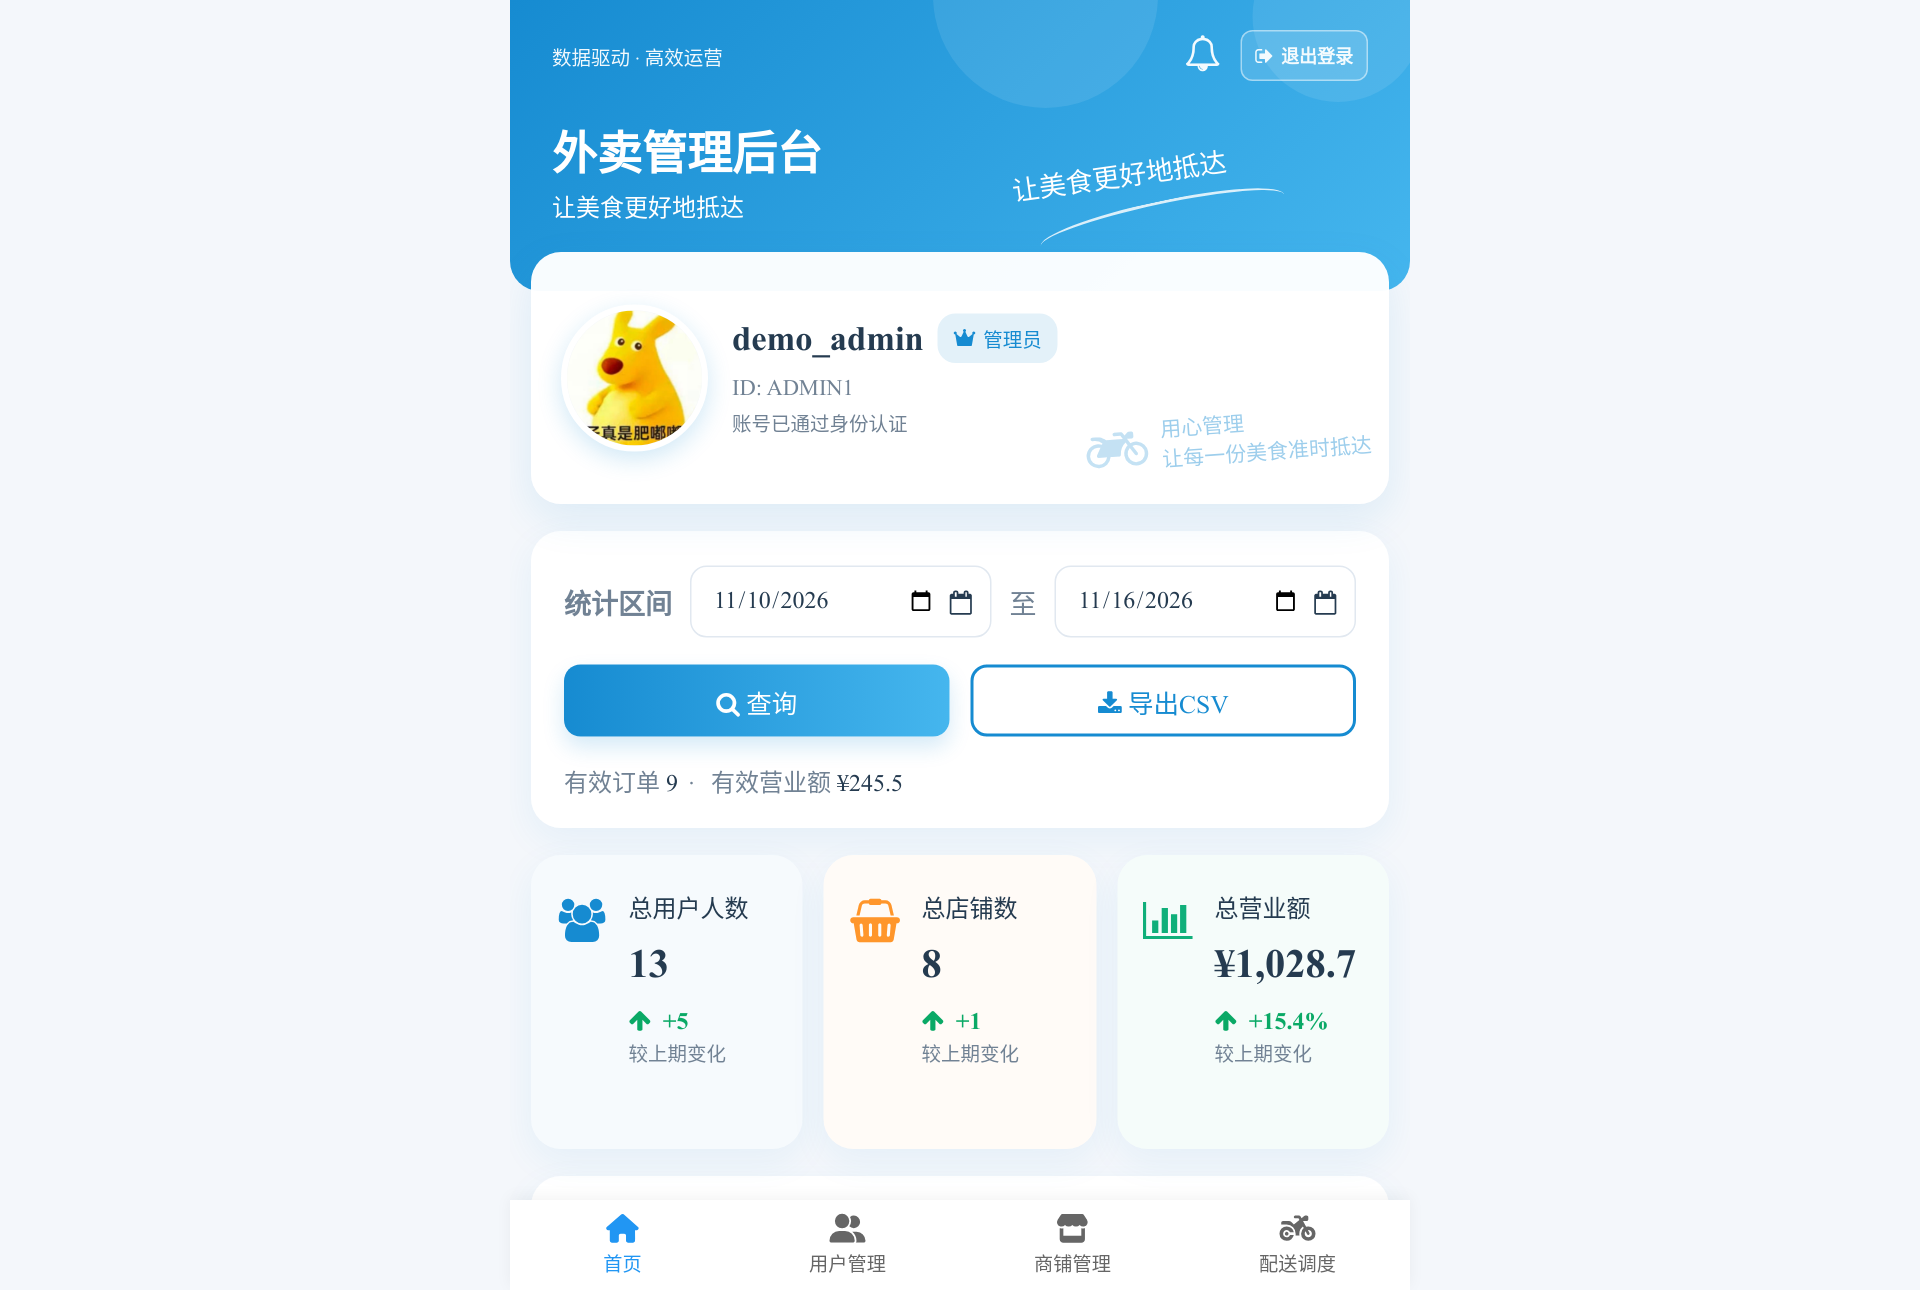
\includegraphics[width=0.96\linewidth,height=0.58\textheight,keepaspectratio]{figures/screenshots/ui-admin-home.png}}
  \caption{管理员端平台全局统计看板桌面运行界面（\code{/admin/home}，支持时间区间检索与 CSV 导出）}\label{fig:def-ui-admin-home}
\end{figure}

\begin{figure}[H]
  \centering
  \fbox{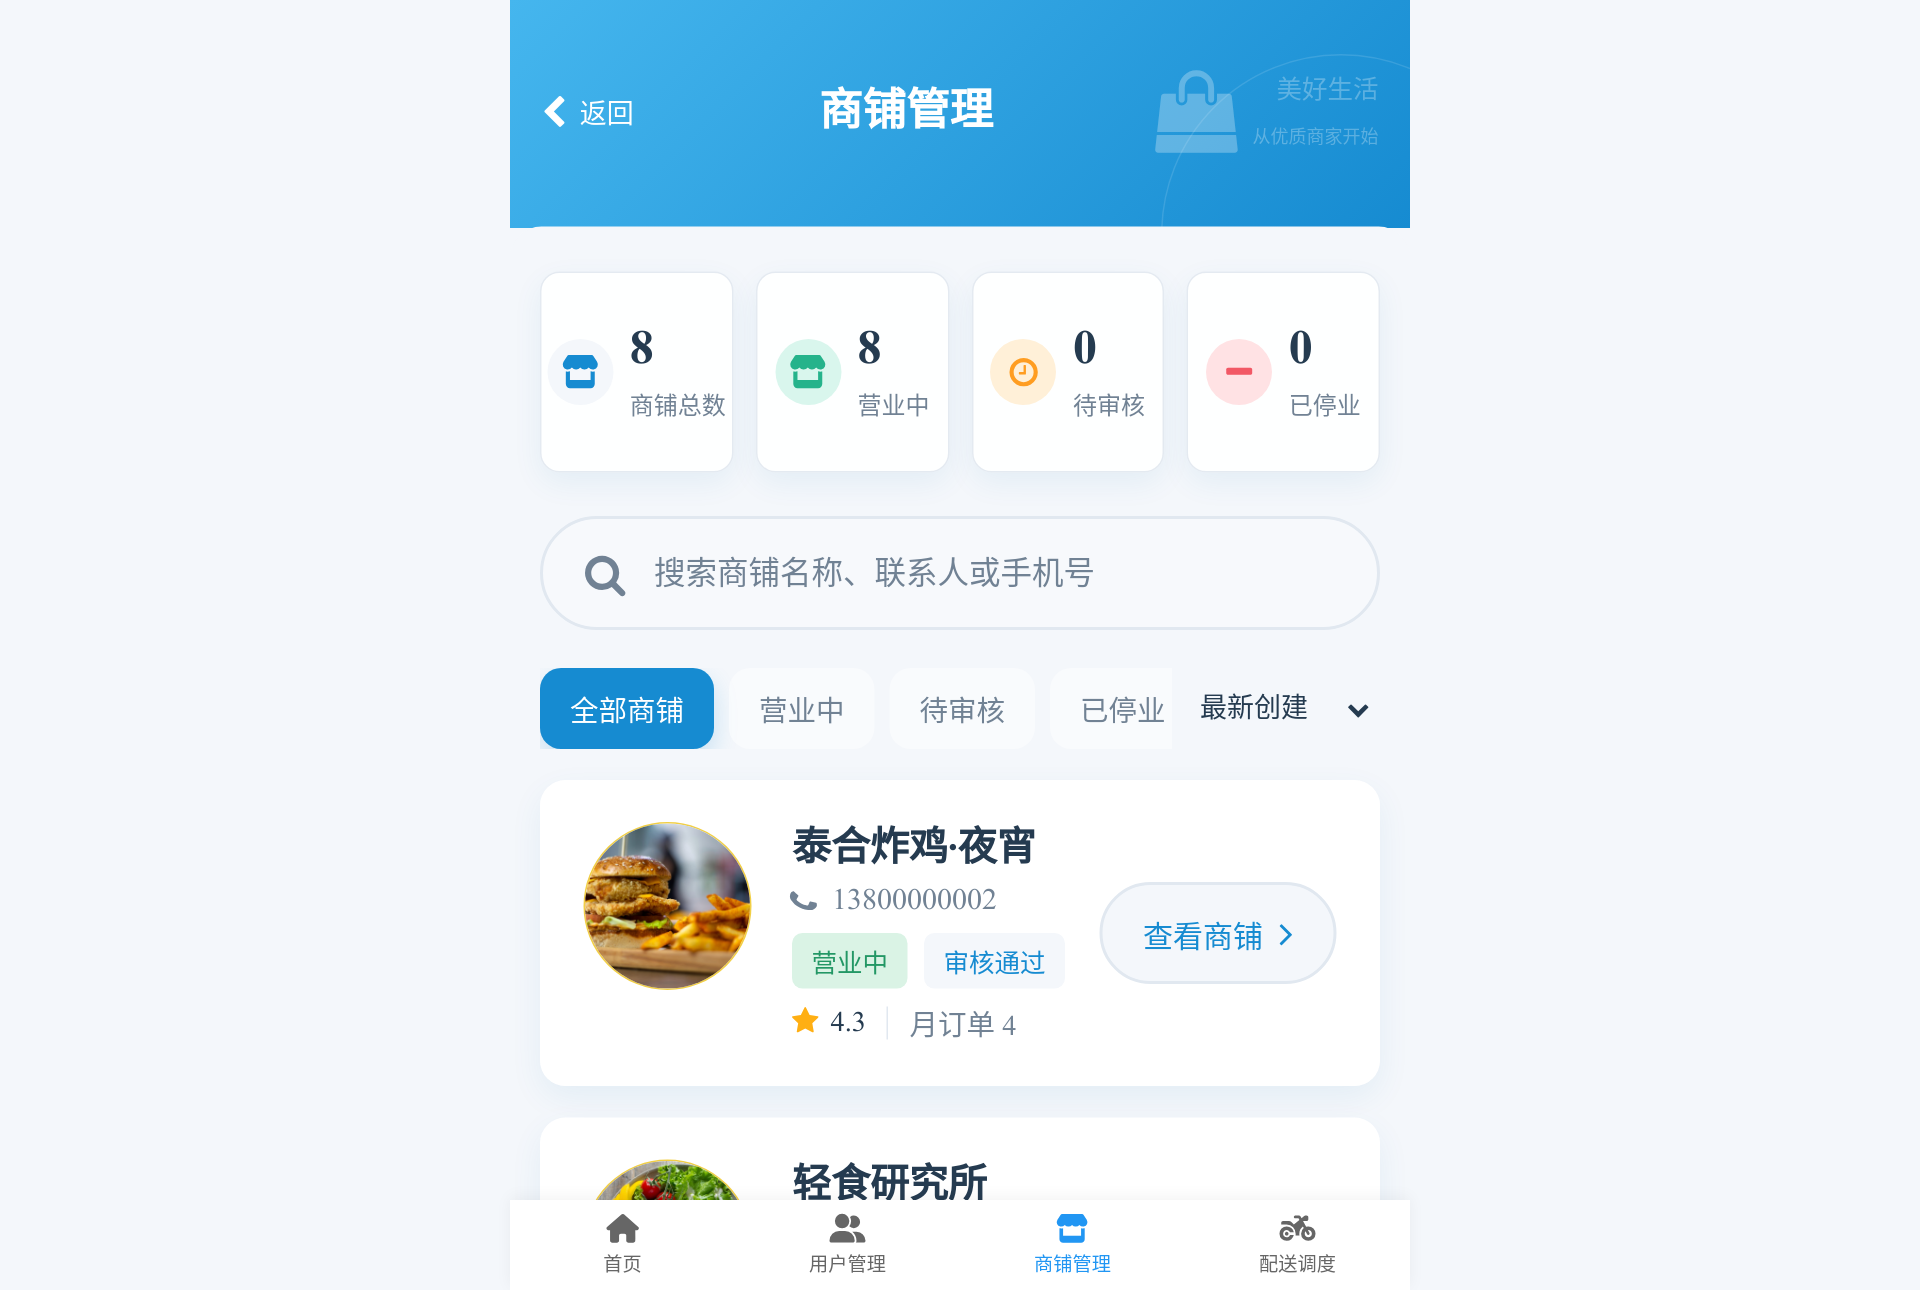
\includegraphics[width=0.96\linewidth,height=0.58\textheight,keepaspectratio]{figures/screenshots/ui-admin-businesses.png}}
  \caption{管理员端商铺入驻审批与营业状态治理界面（\code{/admin/business}）}\label{fig:def-ui-admin-biz}
\end{figure}

\uitwofig{figures/screenshots/ui-admin-users.png}{（a）平台用户账号启停与角色治理（\code{/admin/user}）}{figures/screenshots/ui-admin-riders.png}{（b）骑手入驻审核与配送异常仲裁（\code{/admin/riders}）}{管理员端账号治理与骑手/异常审核界面实景截图}{fig:def-ui-admin-users-riders}

\note{本次服务器未配置高德地图所需的 \code{AMAP_WEB_KEY}、\code{AMAP_JS_KEY} 与 \code{AMAP_SECURITY_CODE}。图~\ref{fig:def-ui-amap} 记录实际打开选址弹窗后出现的“地图服务尚未配置，仍可填写地址”提示，用于展示未配置时的降级状态；该图不作为地图瓦片、POI 搜索或真实定位成功的验证证据。}

\uifig[0.52\linewidth]{figures/screenshots/ui-amap-picker.png}{高德地图选址入口与服务未配置时的实际降级提示界面（\code{/addUserAddress}）}{fig:def-ui-amap}
